\documentclass[master=mai,masteroption=eg,english]{kulemt}
\setup{% Verwijder de "%" op de volgende lijn bij UTF-8 karakterencodering
  %inputenc=utf8,
  title={Short-term forecasting of individual household electrical consumption},
  author={Ir. Stijn Staring},
  promotor={Prof.\,dr.\,ir.\ Bart De Moor},
  assessor={Prof.\,dr.\,ir.\ Unknown\and Prof.\,dr.\,ir.\ Unknown},
  assistant={Ir.\ Lola Botman}}
% Verwijder de "%" op de volgende lijn als je de kaft wil afdrukken
%\setup{coverpageonly}
% Verwijder de "%" op de volgende lijn als je enkel de eerste pagina's wil
% afdrukken en de rest bv. via Word aanmaken.
%\setup{frontpagesonly}

% Kies de fonts voor de gewone tekst, bv. Latin Modern
\setup{font=lm}

% Hier kun je dan nog andere pakketten laden of eigen definities voorzien

% Tenslotte wordt hyperref gebruikt voor pdf bestanden.
% Dit mag verwijderd worden voor de af te drukken versie.
\usepackage[pdfusetitle,colorlinks,plainpages=false]{hyperref}
\usepackage{bm}
\setlength\parindent{0pt}
\usepackage{graphicx}
\graphicspath{{Pictures/}}
\usepackage{amsfonts}
\usepackage{amsmath}
\usepackage{wrapfig}
\usepackage{physics}
\usepackage{booktabs}
\usepackage[ruled,vlined]{algorithm2e}
\usepackage{amsthm}
\usepackage{caption}
\usepackage{subcaption}
\usepackage{gensymb}
\usepackage{textgreek}
\usepackage{bm}
\usepackage[table]{xcolor}
\DeclareMathOperator*{\argmin}{argmin}
%\usepackage{flafter}

%%%%%%%
% Om wat tekst te genereren wordt hier het lipsum pakket gebruikt.
% Bij een echte masterproef heb je dit natuurlijk nooit nodig!
\IfFileExists{lipsum.sty}%
 {\usepackage{lipsum}\setlipsumdefault{11-13}}%
 {\newcommand{\lipsum}[1][11-13]{\par Hier komt wat tekst: lipsum ##1.\par}}
%%%%%%%

%\includeonly{chap-n}
\begin{document}

\begin{preface}
	I am very pleased to present my master thesis to complete my study in Artificial Intelligence. Conducting this research was an informative process in	which I was able to apply the knowledge and skills that I gained during my studies. Writing my thesis and thus completing my studies would not have been possible
	without the support of my mentor Lola Botman, PhD student at the KU Leuven. Thank you for the interesting meetings and brainstorm sessions we had. Also, I would like to thank my family for their ongoing support during all phases of my studies. They have always been my biggest fans and I could not have done this without the opportunities they have given me. At last, I want to thank everybody that reads this text. Sit back, relax and enjoy.
\end{preface}

\tableofcontents*

\begin{abstract}
  The \texttt{abstract} environment contains a more extensive overview of
  the work. But it should be limited to one page.

\end{abstract}

%\begin{abstract*}
%  In dit \texttt{abstract} environment wordt een al dan niet uitgebreide
%  Nederlandse samenvatting van het werk gegeven.
%  Wanneer de tekst voor een Nederlandstalige master in het Engels wordt
%  geschreven, wordt hier normaal een uitgebreide samenvatting verwacht,
%  bijvoorbeeld een tiental bladzijden. 
%
%\end{abstract*}

% Een lijst van figuren en tabellen is optioneel
%\listoffigures
%\listoftables
% Bij een beperkt aantal figuren en tabellen gebruik je liever het volgende:
\listoffiguresandtables
% De lijst van symbolen is eveneens optioneel.
% Deze lijst moet wel manueel aangemaakt worden, bv. als volgt:
%\chapter{List of Abbreviations and Symbols}
%\section*{Abbreviations}
%\begin{flushleft}
%  \renewcommand{\arraystretch}{1.1}
%  \begin{tabularx}{\textwidth}{@{}p{12mm}X@{}}
%    LoG   & Laplacian-of-Gaussian \\
%    MSE   & Mean Square error \\
%    PSNR  & Peak Signal-to-Noise ratio \\
%  \end{tabularx}
%\end{flushleft}
%\section*{Symbols}
%\begin{flushleft}
%  \renewcommand{\arraystretch}{1.1}
%  \begin{tabularx}{\textwidth}{@{}p{12mm}X@{}}
%    42    & ``The Answer to the Ultimate Question of Life, the Universe,
%            and Everything'' according to \cite{h2g2} \\
%    $c$   & Speed of light \\
%    $E$   & Energy \\
%    $m$   & Mass \\
%    $\pi$ & The number pi \\
%  \end{tabularx}
%\end{flushleft}

% Nu begint de eigenlijke tekst
\mainmatter

\chapter{Introduction}
\label{cha:intro}









\section{Importance of topic}
Individual household forecasting is a complex task because of the high amount of uncertainty
and the volatility of the data. To deal with this it was found in literature that often aggregated signals are forecasted instead. If there are papers that discuss electrical household consumption forecasting, they often use a lot of information about the household which will not be scalable in practice due to privacy concerns. This thesis investigates state of the art time series forecasting techniques based on LSTM neural networks that have as goal to forecast the next day of electrical household consumption, given only limited information.\\

When forecasting is improved on household scale, the customer can be better informed what the bill is going to be at the end of the month/year.
Energy producer can build a better trust with its customer by sending reliable bills. (Providing good service)
Producent can better estimate the energy demand of the whole customer population. This will lead to cheaper electricity production because a better planning is possible where there is less need of the more 
flexible but more expensive electricity installations e.g. diesel engines.

\section{Problem formulation and link with previous studies}
Now going to forecast individual houses, not aggregated signals. 


\section{Thesis objective and structure}
The goal of this thesis is to do short-term load forecasting for individual households. A forecast of the electrical load of a household for 24 hours. 

%%% Local Variables: 
%%% mode: latex
%%% TeX-master: "thesis"
%%% End: 

\chapter{Exploratory Data Analysis}
\label{cha:Data analysis}
This chapter starts by describing the dataset were the exploratory data analysis will be performed on in Section \ref{s:Data description}. Next, the preprocessing steps done before the data analysis are explained in Section \ref{s:Preprocessing}. The preprocessing steps consists out of handling missing data, identifying zero days, normalization and removing time series with a big shift in its rolling mean for all the 261 load series with a full year of smart meter measurements. In Section \ref{s:Data Analysis} follows a data analysis on the preprocessed data. For this all the 261 load series with a full year of smart meter measurements are aggregated to identify general characteristics of the data. Things of the aggregated load serie that are assessed are seasonality, comparing electrical consumption between weekdays and weekends, impact of an holiday, the influence of the temperature and the identification of the influence of properties of the household e.g. dwelling type. This last part was possible due to the availability of extra information through a voluntary questionnaire.


\section{Data description}\label{s:Data description}
The data used in this thesis was made available for the \href{https://ieee-dataport.org/competitions/ieee-cis-technical-challenge-energy-prediction-smart-meter-data}{IEEE-CIS technical challenge on energy prediction from smart data}. The dataset consists of load signals with time steps of 30 minutes of 3248 households located in the UK during the year 2017. Only households are considered and no The definition of an household are all the people who occupy a single housing unit, regardless of their relationship to one another. Each smart meter is property of E.ON UK and can collect a maximum  of $17520$ measurements during the year 2017.
 Not all the $3248$ smart meters consist out of full data as can be seen in Figure \ref{fig:amountNaN}. It can be clearly seen that there are $12$ jumps in the amount of missing values. This is because the available data ranges from one month (only December) to a full year of data. This acknowledges that customers may have joined the measuring campaign at different times during the year. There are additional missing values in the time series due to sending or receiving errors of the smart meter.\\
 
 \begin{figure}[h!]
 	\centering
 	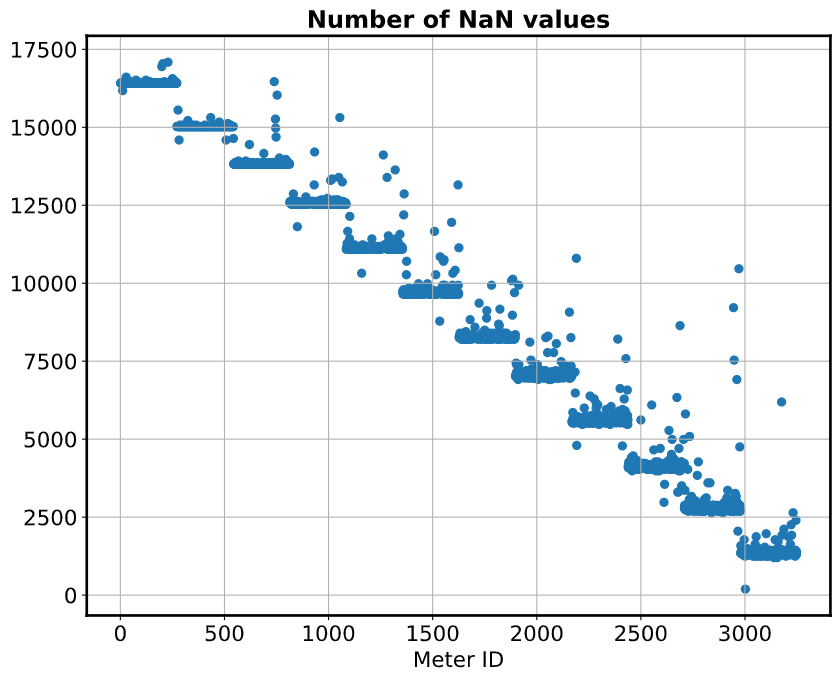
\includegraphics[width=0.8\textwidth]{amountNaN.png}
 	\caption{The amount of NaN values in all the 3248 load signals.}
 	\label{fig:amountNaN}
 \end{figure}

Besides of the electricity consumption of the different households, also information is available about the average, minimum and maximum temperatures on a daily resolution. Finally, extra household information has been partially collected about 2143 households through voluntary surveys. This concerns the dwelling type, number of occupants, number of bedrooms etc. as further detailed in Table \ref{tab:attributes}. From the questionnaire it can be derived that the maximum amount of residents is 4 and there is a maximum amount of bedrooms of 5. The kind of house units are: flat, bungalow, detached house, semi detached house and terraced house. Industrial loads or small businesses e.g. a bakery is not considered. The available datasets and their features are summarized by Table \ref{tab:available_data}.\\

\begin{table}[h]%\[!htb\]	
	\raggedright
	\begin{tabular}[t]{@{}ll}
		\firsthline
		\textbf{Consumption.csv}&\\ \hline
		\# households &3248 \\ 
		Information & Electric load\\
		Max measurements/serie & 17520\\
		Granularity&$ 1/2$ hour\\ 
		Timespan&year 2017 \\    
		Location&UK\\ \bottomrule   
	\end{tabular}
	\hfill
	\raggedleft
	\begin{tabular}[t]{@{}ll}
		\firsthline
		\textbf{Weather.csv}&\\ \hline
		Information & Average temperature\\
		& Max temperature\\
		& Min temperature\\
		Granularity& daily\\ \hline
		\textbf{addInfo.csv}&\\ \hline
		\# households &2143 \\ \bottomrule		    
	\end{tabular}\\
	\caption{Summary of the available csv files form the IEEE-CIS technical challenge.}
	\label{tab:available_data}
\end{table}




\section{Preprocessing}\label{s:Preprocessing}

Following sections describe the preprocessing applied on the 261 load series containing measurements for the entire year. The preprocessing done here is in preparation of the data analysis of Section \ref{s:Data Analysis}. It must not be confused with the preprocessing done for the three considered load series in Chapter \ref{cha:Forecasting the daily electricity consumption}.

\subsection{Missing data} \label{s:missing_data}
As discussed in Section \ref{s:Data description}, there exists two types of missing data in the Consumption csv file as was stated in the data description of the competition: fully missing months, due to the later participation in the measuring campaigns and missing values due to sending or receiving errors of the smart meter. When a smart meter fails, always all the measurements of that day are lost. In this Section two methods to impute the missing values are compared. Method Average Neighbours: replaces a missing value by the mean of the consumption values at the same moment on the next and previous days. Method Mean: substitutes the missing values of a time serie by the mean of all the measurements done by the meter. If the next or previous day is also missing in the serie, two days forward or back in time are used to replace the unknown day and so on. The resulting imputed signals can be seen in Figure \ref{fig:missing_values_imputing}. \\

\begin{figure}[h]
	\begin{subfigure}{0.5\textwidth}
		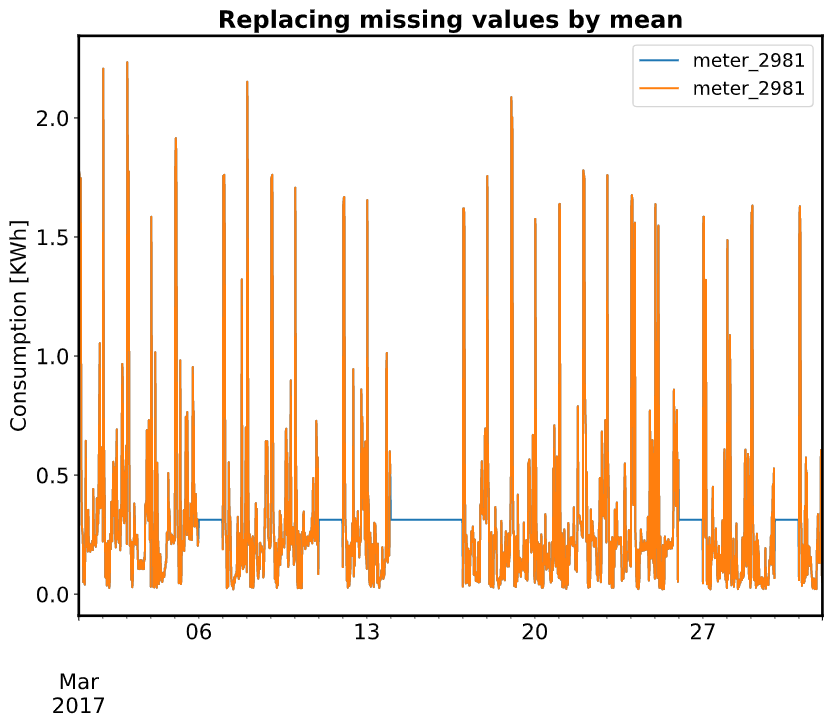
\includegraphics[width=1\linewidth]{mv_mean.png}
		\caption{Mean}
	\end{subfigure}	
	\begin{subfigure}{0.5\textwidth}
		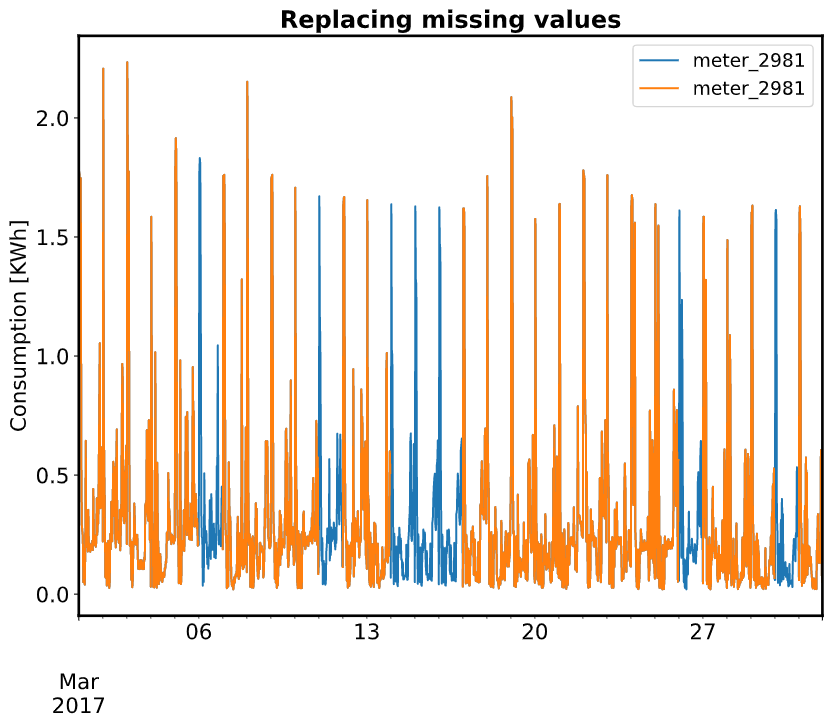
\includegraphics[width=1\linewidth]{mv_s.png}
		\caption{Average Neighbours}
	\end{subfigure}
	\caption{Resulting time serie of the month March after imputation of the missing data.}
	\label{fig:missing_values_imputing}
\end{figure}

In order to compare how accurate both methods impute missing values, 181 months of March without any missing values were used and in each month randomly 7 days were removed. After applying both imputation methods, the resulting estimated signal was compared with the original one and an error value between both signals is calculated, using the mean squared error metric. Normalization is done by dividing the calculated MSE's by the MSE of the worst performing method to calculate the percentage of improvement of one method in comparison to the other. Figure \ref{fig:mv_result} shows that on average, a reduction of the MSE of more then $ 20\% $ is achieved when the average neighbours method is used in comparison to the mean method. Therefore, the average neighbours method will be applied to impute the missing values of the 261 time series with a full year of smart meter measurements. The only exception is made when the first of January and thirty-one December are imputed. Because not both neighbouring days can be known, the mean method is used.

\begin{figure}[h!]
	\centering
	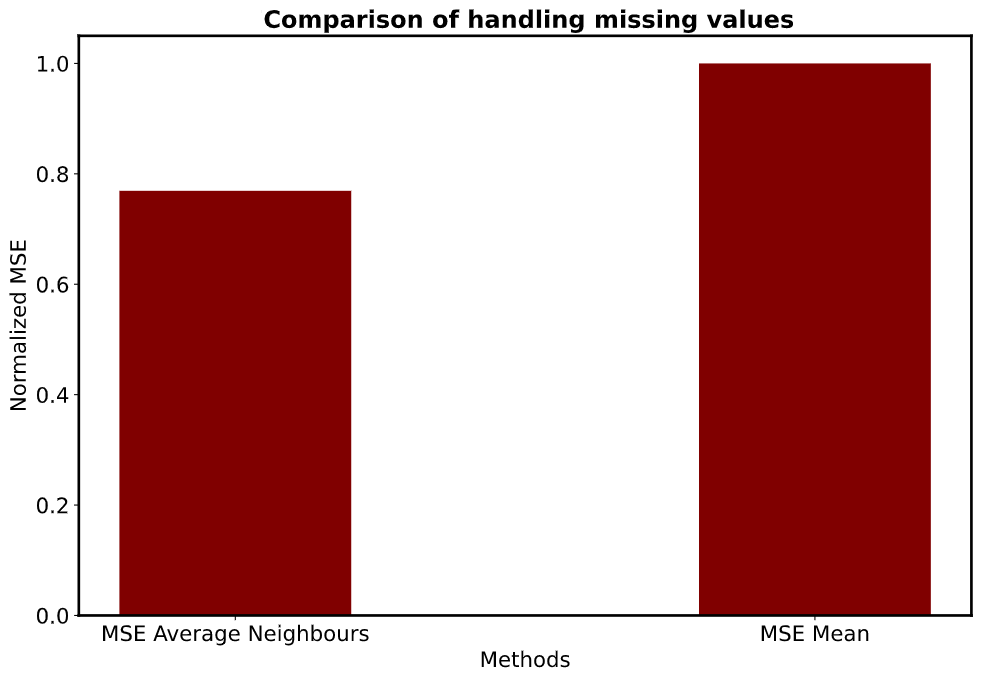
\includegraphics[width=0.8\textwidth]{mv_result.png}
	\caption{Resulting month of March after substitution of the missing values by the mean value of the measurements. }
	\label{fig:mv_result}
\end{figure}

%Actually, used the missing values a bit at random. First imputed the missing values using the average neighbours method and later during the forecasting phase, used different imputation techniques that were not compared with the initial imputation techniques.


\subsection{Zero days}

When inspecting the load series, some untraditional meter measurements were identified. There were $ 9 $ meters of the 261 that had more than one day with a total electrical consumption of zero. Because it is unlikely that a household produces exactly zero kWh on an entire day all these $ 9 $ meters were removed. One of 9 load series is compared in Figure \ref{fig:zero_con} with a load serie with zero days and it is clear that the horizontal lines are not part of a normal household load signal.

\begin{figure}[ht]
	\begin{subfigure}{0.49\textwidth}
		\vspace{4mm}
		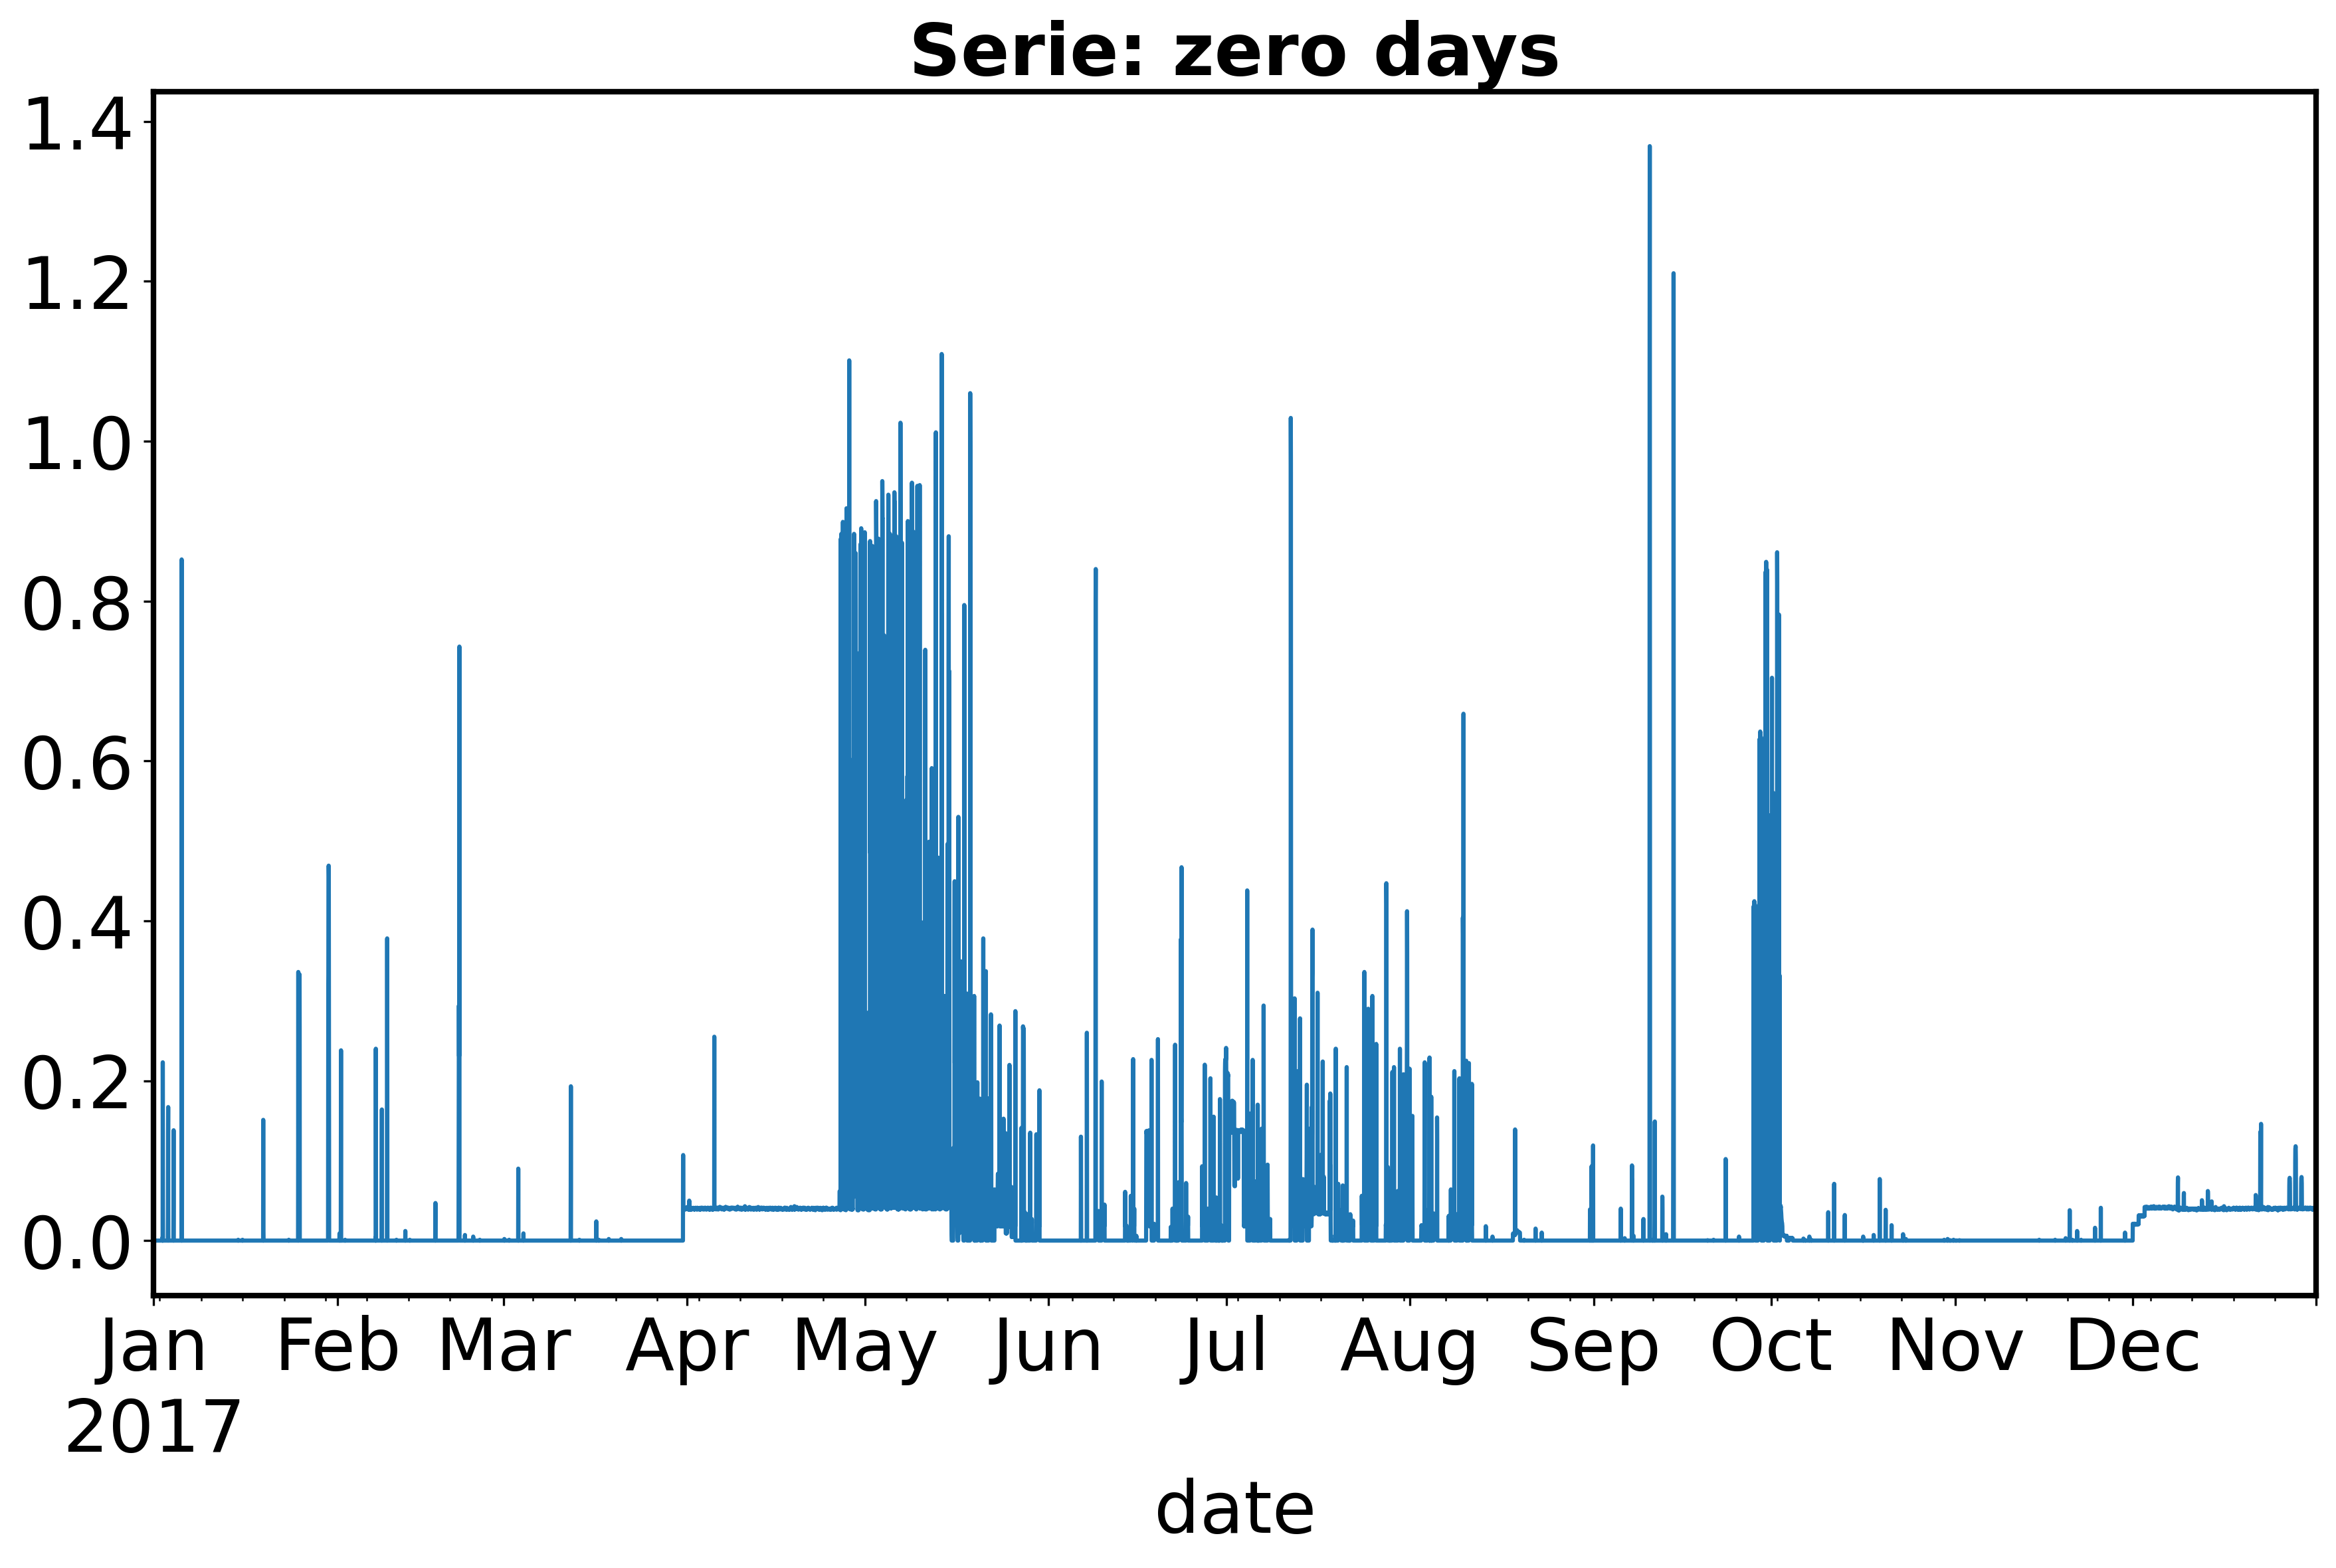
\includegraphics[width=1\linewidth]{zero_days.png}
		\caption{Serie with more than one day with zero consumption.}
	\end{subfigure}	 	
	\begin{subfigure}{0.49\textwidth}
		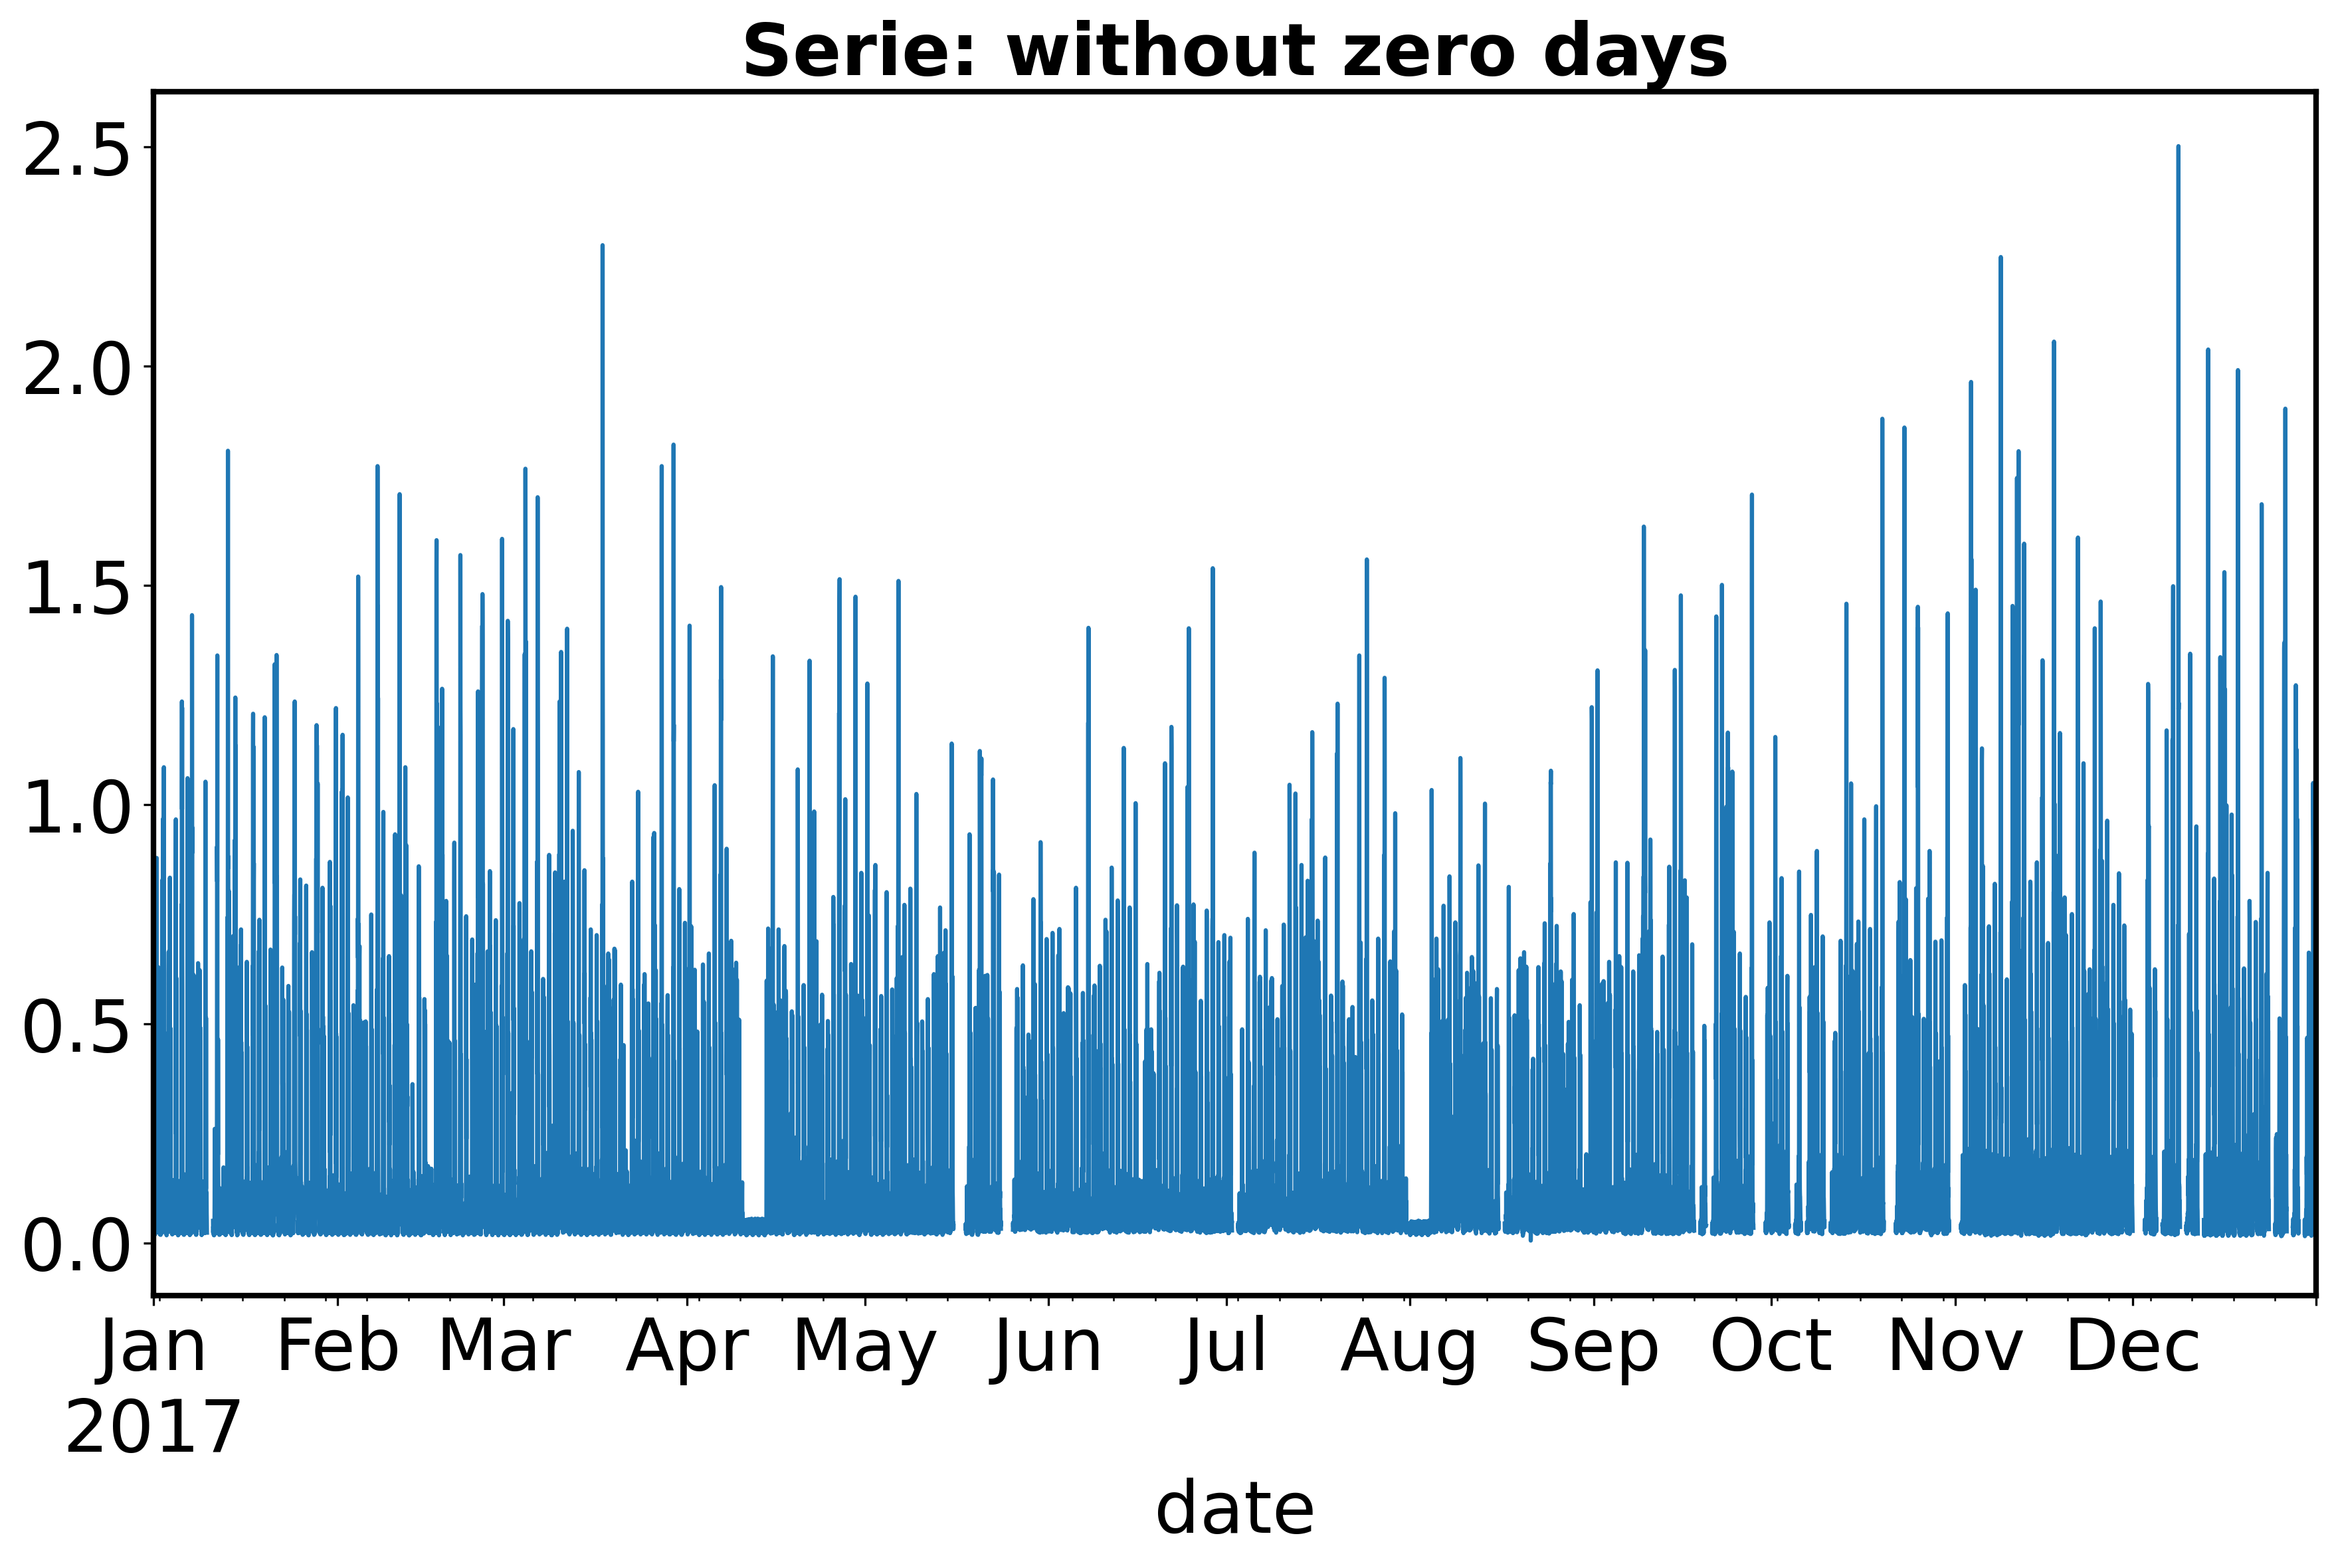
\includegraphics[width=1\linewidth]{without_zero_days.png}
		\caption{Serie $ 2 $ from Chapter \ref{cha:Forecasting the daily electricity consumption}.}
	\end{subfigure}	
	\caption{Comparison of series with and without zero load days.}
	\label{fig:zero_con}
\end{figure}

\subsection{Normalization of the data}
\label{s:Normalization of the data}
% normalize as done in ppt --> deviding by the yearly consumption.
% downside of this normalilzation that outshooters will have influence.
Normalization is necessary because while absolute consumption differs, relative patterns of human behaviour can be more similar according to \cite{Lago2020}. The goal of a forecasting model applied on an individual household is to extract the human behaviour and normalization contributes to this by avoiding the disturbance of different magnitudes in which this human pattern may occur. Every load serie is normalized based on its yearly consumption as was done by \cite{Lago2020}. The advantage of using the yearly consumption for normalization in comparison to the min-max method often used in literature, is the robustness against measurement outliers. This is important because in Section \ref{s:Data Analysis} all the 261 time series will be aggregated, which means that when a serie has only one very large outlier, the rest of its consumption values will be observed as small values in comparison with other series without a very large outlier. This is avoided when using the yearly consumption normalization where every load serie will be one at the end of the year as shown by Eq. \ref{eq:norm}. This allows for better comparison among the different series. The min-max normalization method is however used in Chapter \ref{cha:Forecasting the daily electricity consumption}, but here the series are always assessed individually

\begin{equation}\label{eq:norm}
	normalized\hspace{0.3cm} consumption_i = \frac{consumption_i}{\sum_{k=1}^{17520} consumption_k}.
\end{equation} 


\subsection{Shifts in rolling mean of load signal} \label{s:Shifts in rolling mean of load signal}
In this Section the normalized time series are assessed on fundamental changes in the load signal which can't be explained by normal human behaviour in the current household setting. A fundamental change of the load signal can be caused by an extra inhabitant or when systems are installed during the year that use a lot of electricity e.g. air-conditioning. A fundamental change is identified by looking at the maximum difference of the maximum and minimum rolling mean consumption over $ 7 $ days. Figure \ref{fig:fund_change} shows all the maximum differences between the maximum and minimum weekly rolling averages for the 261 load series. Outliers in the the maximum difference are detected as is done in a boxplot, namely from the third quartile a distance of one and a half times the interquartile range is added and values higher are considered as outliers. The red line in Figure \ref{fig:fund_change} shows when a maximum difference is considered as an outlier. Finally, the outliers which corresponds to 5 load series above the red line, are removed because they are seen as a disturbance when the load signals are aggregated in Section \ref{s:Data Analysis}. Figure \ref{fig:rolling_mean_shift} shows one of the removed load signals. 

\begin{figure}[h!]
	\centering
	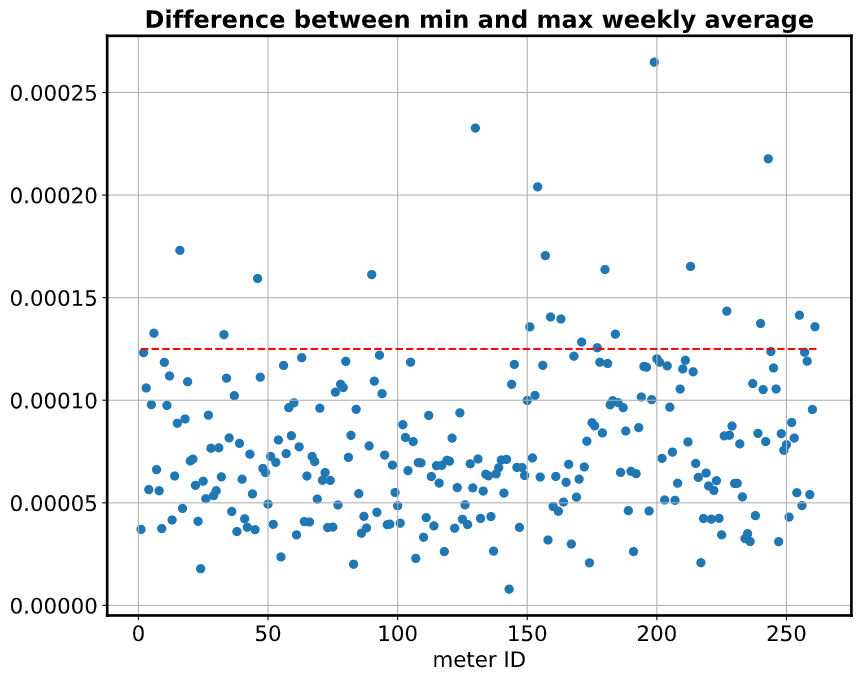
\includegraphics[width=0.8\textwidth]{fund_change.png}
	\caption{The maximum differences between the maximum and minimum weekly rolling mean for all the 261 different load signals.}
	\label{fig:fund_change}
\end{figure}


\begin{figure}[h!]
	\centering
	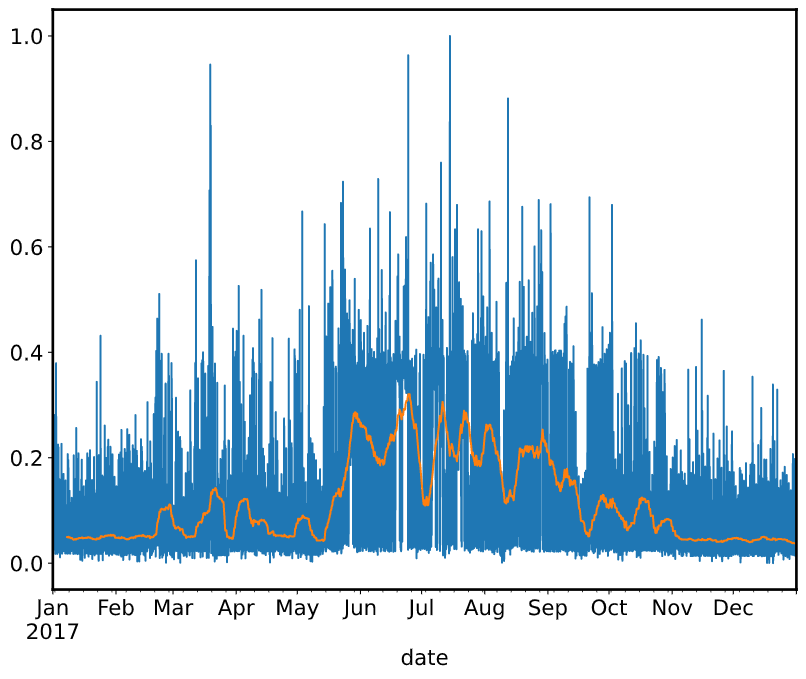
\includegraphics[width=0.8\textwidth]{fundamental_change.png}
	\caption{Removed load signal with a shift in the rolling mean.}
	\label{fig:rolling_mean_shift}
\end{figure}


\section{Data Analysis}\label{s:Data Analysis}
In this section the remaining $256$ time series are converted to a single load serie by taking the mean. The single load serie is further referenced as the mean signal. This is done to identify general characteristics of the data. Things that are going to be assessed are: seasonality, comparing electrical consumption between weekdays and weekends, impact of an holiday, the influence of the temperature and the influence of properties of the household e.g. dwelling type.


% An individual household consumption time-serie is much subdued to complex and personal decisions that cause increases or decreases of the consumption. It is hard to capture all theses effects in a single model. By aggregation of the individual time-series by taking the average, this noisy individual behaviour is mitigated. The aggregated signal is now modelled and the increase or decrease of the consumption can be explained by a small set of variables. The aggregated signal can be seen as a ``virtual distribution substation'' as discussed in \cite{Hoverstad2015}. 
 
\subsection{Seasonality}
In \cite{Hoverstad2015} it is concluded that all the forecasting algorithms that were considered, produced more accurate forecasts when they were combined with a preprocessing stage that extracted the seasonality before forecasting, compared to applying the same algorithms directly on raw data. The forecasting model is left with the task of modelling the deviation from the template consumption instead of performing a forecast out of the blue. However in \cite{Hoverstad2015} they made forecasts of an aggregated signal which had a reasonable amount of regularity which is not the case for electrical consumption forecasting of individual households. That it is not useful to extract a regular pattern is in accordance to \cite{Shi2018}, where it is explained that the use of a spectral analysis such as a wavelet analysis, that aims at separating the regular pattern from the uncertainty and the noise, is not applicable during load forecasting of individual households due to the low amount of regularity. However, the analyses of the seasonality of the mean signal is still informative to get a feeling of the general human behaviour.\\

These day and week templates are extracted from the mean signal by the use of equations \ref{eq:daily_filter} and \ref{eq:weekly_filter} that calculate respectively the average day and week indicated by a thick blue line in Figure \ref{fig:average_signals}.

\begin{equation}\label{eq:daily_filter}
	\bar{y}_i = \frac{1}{D} \sum_{d=1}^D y_{d,i}, \hspace{10mm} i \in [1,48],
\end{equation} 

\begin{equation}\label{eq:weekly_filter}
	\bar{y}_j = \frac{1}{W} \sum_{w=1}^W y_{w,j}, \hspace{10mm}  j \in [1,336].
\end{equation} 

 $ D $ and $ W $ give respectively the amount of days and weeks in the year 2017. $\bar{y}_i$ and $\bar{y}_j$ give the consumption of half an hour, averaged over respectively all days and weeks. In Figure \ref{fig:average_signals} a clear consumption peak can be seen after midnight. This is due to heat storage systems that use electricity in the hours of low tariff and that release heat during high electricity tariffs. The daily seasonality shows a small peak in the load around 7 am and a bigger one around 6 pm. In the weekly seasonality it can be seen that all the peaks at 6 pm are of the same height but the smaller peak is different depending if it is a weekday or weekend as will be further explained in Section \ref{s:Comparing weekdays with weekends}. 

\begin{figure}[h!]
	\begin{subfigure}{1.0\textwidth}
		\centering
		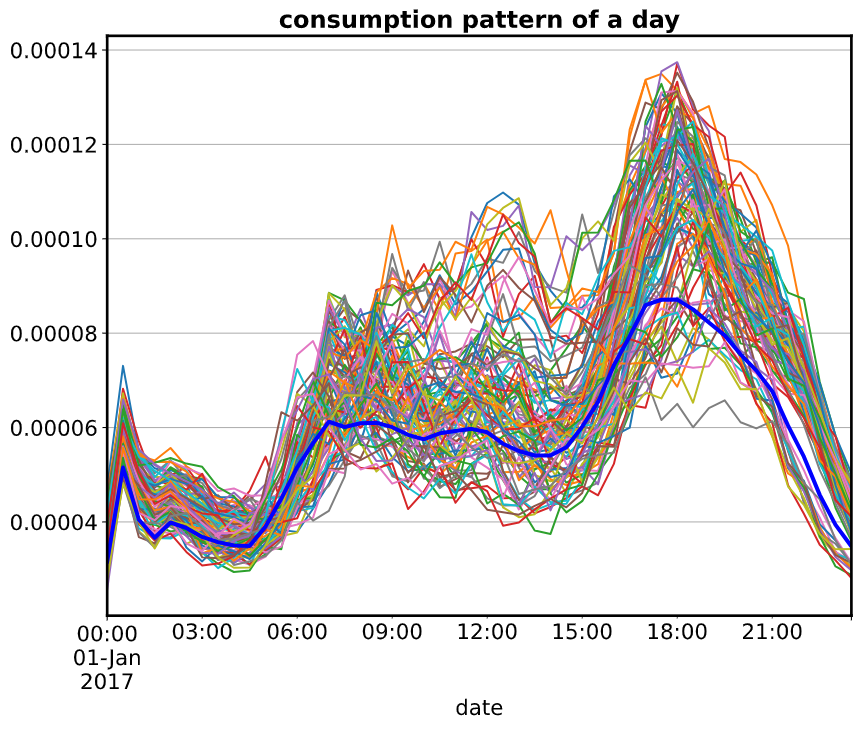
\includegraphics[width=0.7\linewidth]{daily_filter.png}
		\caption{Daily seasonality}
	\end{subfigure}	 	
	\begin{subfigure}{1.0\textwidth}
		\centering
		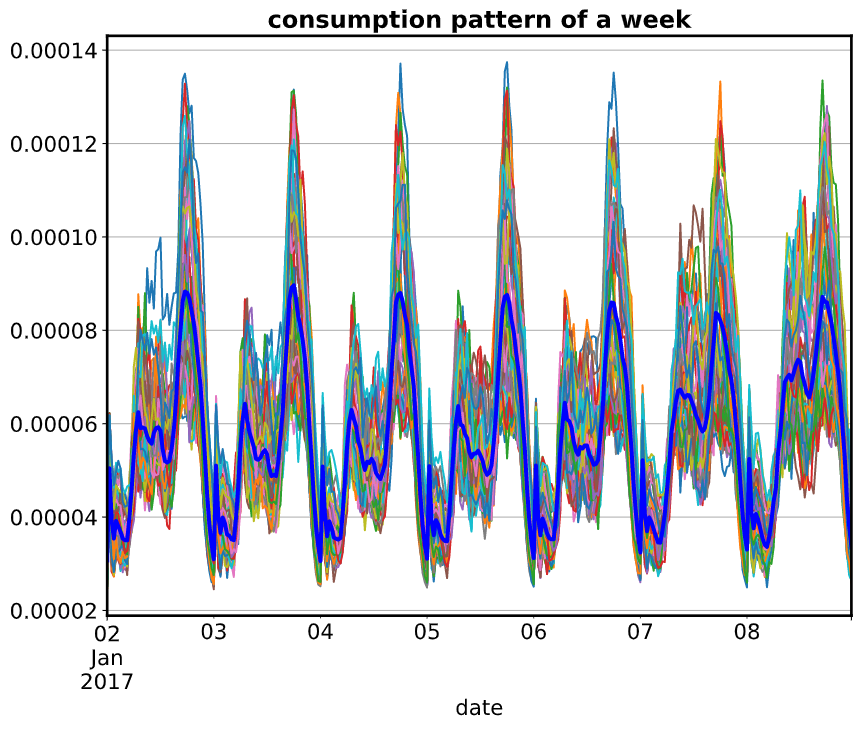
\includegraphics[width=0.7\linewidth]{weekly_filter.png}
		\caption{Weekly seasonality}
	\end{subfigure}	
	\caption{The seasonality of the electrical load during the year 2017. The blue line indicates the average load signal. }
	\label{fig:average_signals}
\end{figure}


% plot the moving average of the year. Clearly see the impact of the summer and winter.
% This is a trend that can be taken into account when predicting.



\subsection{Comparing weekdays with weekends} \label{s:Comparing weekdays with weekends}
Weekdays and weekends are compared with the help of Figure \ref{fig:average_signals}. It is clear that the consumption of the average business day is similar to a weekend day considering the time of three two peaks each day. There is a morning peak around 7 am, an evening peak around 6pm and a peak after midnight. However, in the weekends, the morning peaks seems to be a little higher and decreases less. The effect can be seen during both weekend days, but is most visible on the Sundays. To prove previous statements, the similarity is assessed by calculating the normalized MAE is calculated for the hourly difference of each combination of 2 days of the week. Normalization is done by dividing the different MAE's by the biggest MAE calculated. Figure \ref{fig:similarity_weekdays} shows in blue and orange the error of combinations between business days or weekend days and in green the error of combinations between a business day and weekend day. It can be clearly seen that when a business day and weekend day are combined (green) the error is larger and thus more dissimilar. The left cluster of dots corresponds to a Saturday that is combined with a weekday and the right cluster corresponds to a Sunday combined with a weekday. It can be noticed that Saturdays are more similar to a business day than a Sundays. 

\begin{figure}[h!]
	\centering
	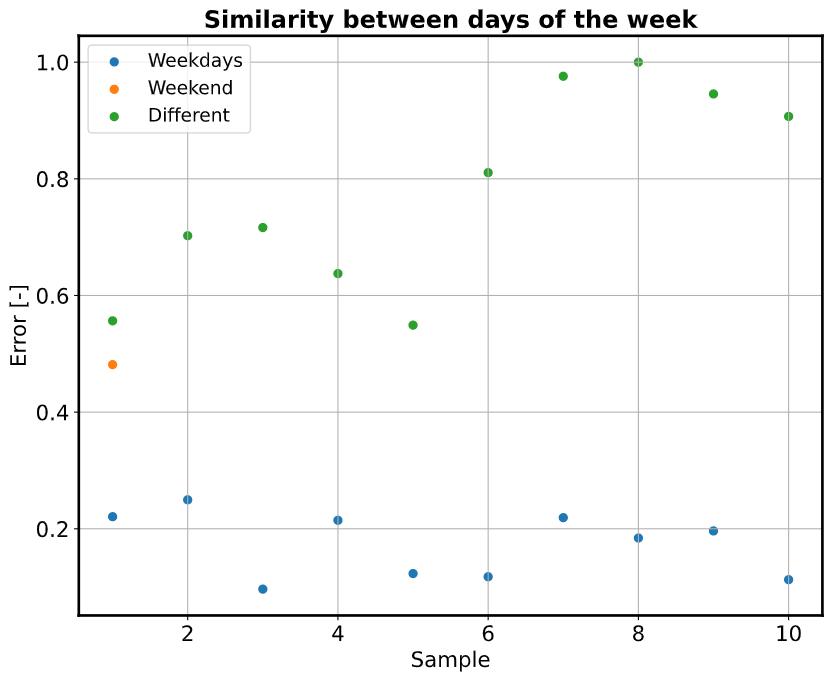
\includegraphics[width=0.8\textwidth]{similarity_weekdays.png}
	\caption{Error between different pairs of weekdays.}
	\label{fig:similarity_weekdays}
\end{figure}

\subsection{Impact of bank holidays}\label{s:Impact of holidays}
% important that look at holidays in the UK. In paper \cite{Hoverstad2015} all the holydays are subsitued by the same day the next week and the previous week. It is possible to look at all the holidays, normalize them concerning temperature and try to get a seasonality model. 
In order to look at the impact of a bank holiday, all the holidays of the English and Welsh calendar are identified for the year $ 2017 $. For each of the $ 8 $ bank holidays a corresponding business day is selected with an in euclidean distance as close as possible average temperature of the day. Therefore, mitigating the temperature influence. Note that each of the 8 holidays or business days are from the mean signal and they therefore are already averaged over 256 load signals. The 8 bank holidays and business days are averaged to obtain Figure \ref{fig:bvsj}. It is observed that a bank holiday behaves similarly to a weekend day which means a higher morning peak that decreases less. Figure \ref{fig:sim_weekdays} illustrates the similarity between a holiday and the days of the week. The error is calculated as the MAE of the hourly difference between the average day of the week and holiday. It can be seen that a bank holiday behaves most similarly to a Sunday.

\begin{figure}[h!]
	\centering
	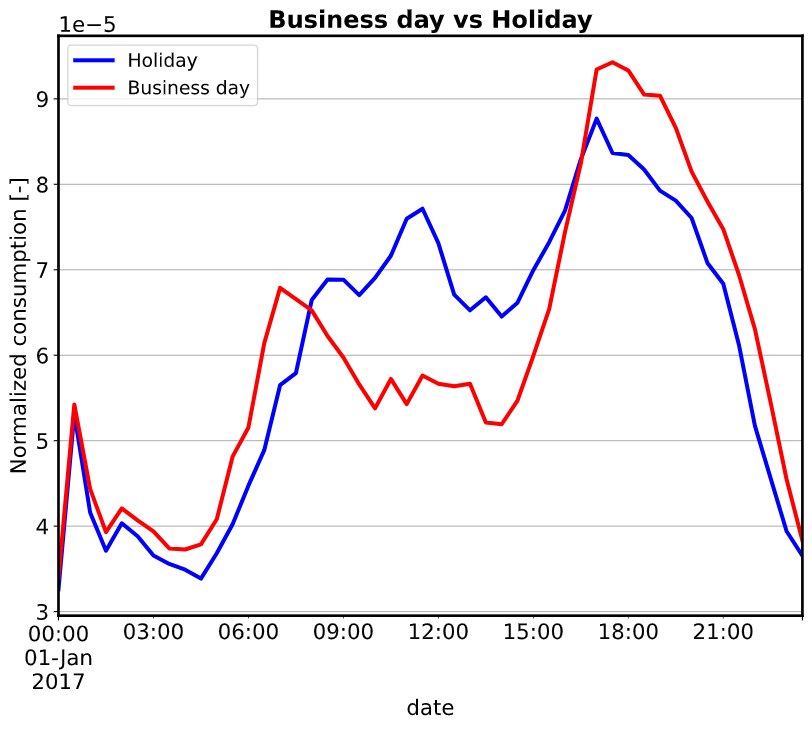
\includegraphics[width=0.6\textwidth]{bvsh.png}
	\caption{Comparison between bank holiday and business day electrical consumption.}
	\label{fig:bvsh}
\end{figure}

\begin{figure}[h!]
	\centering
	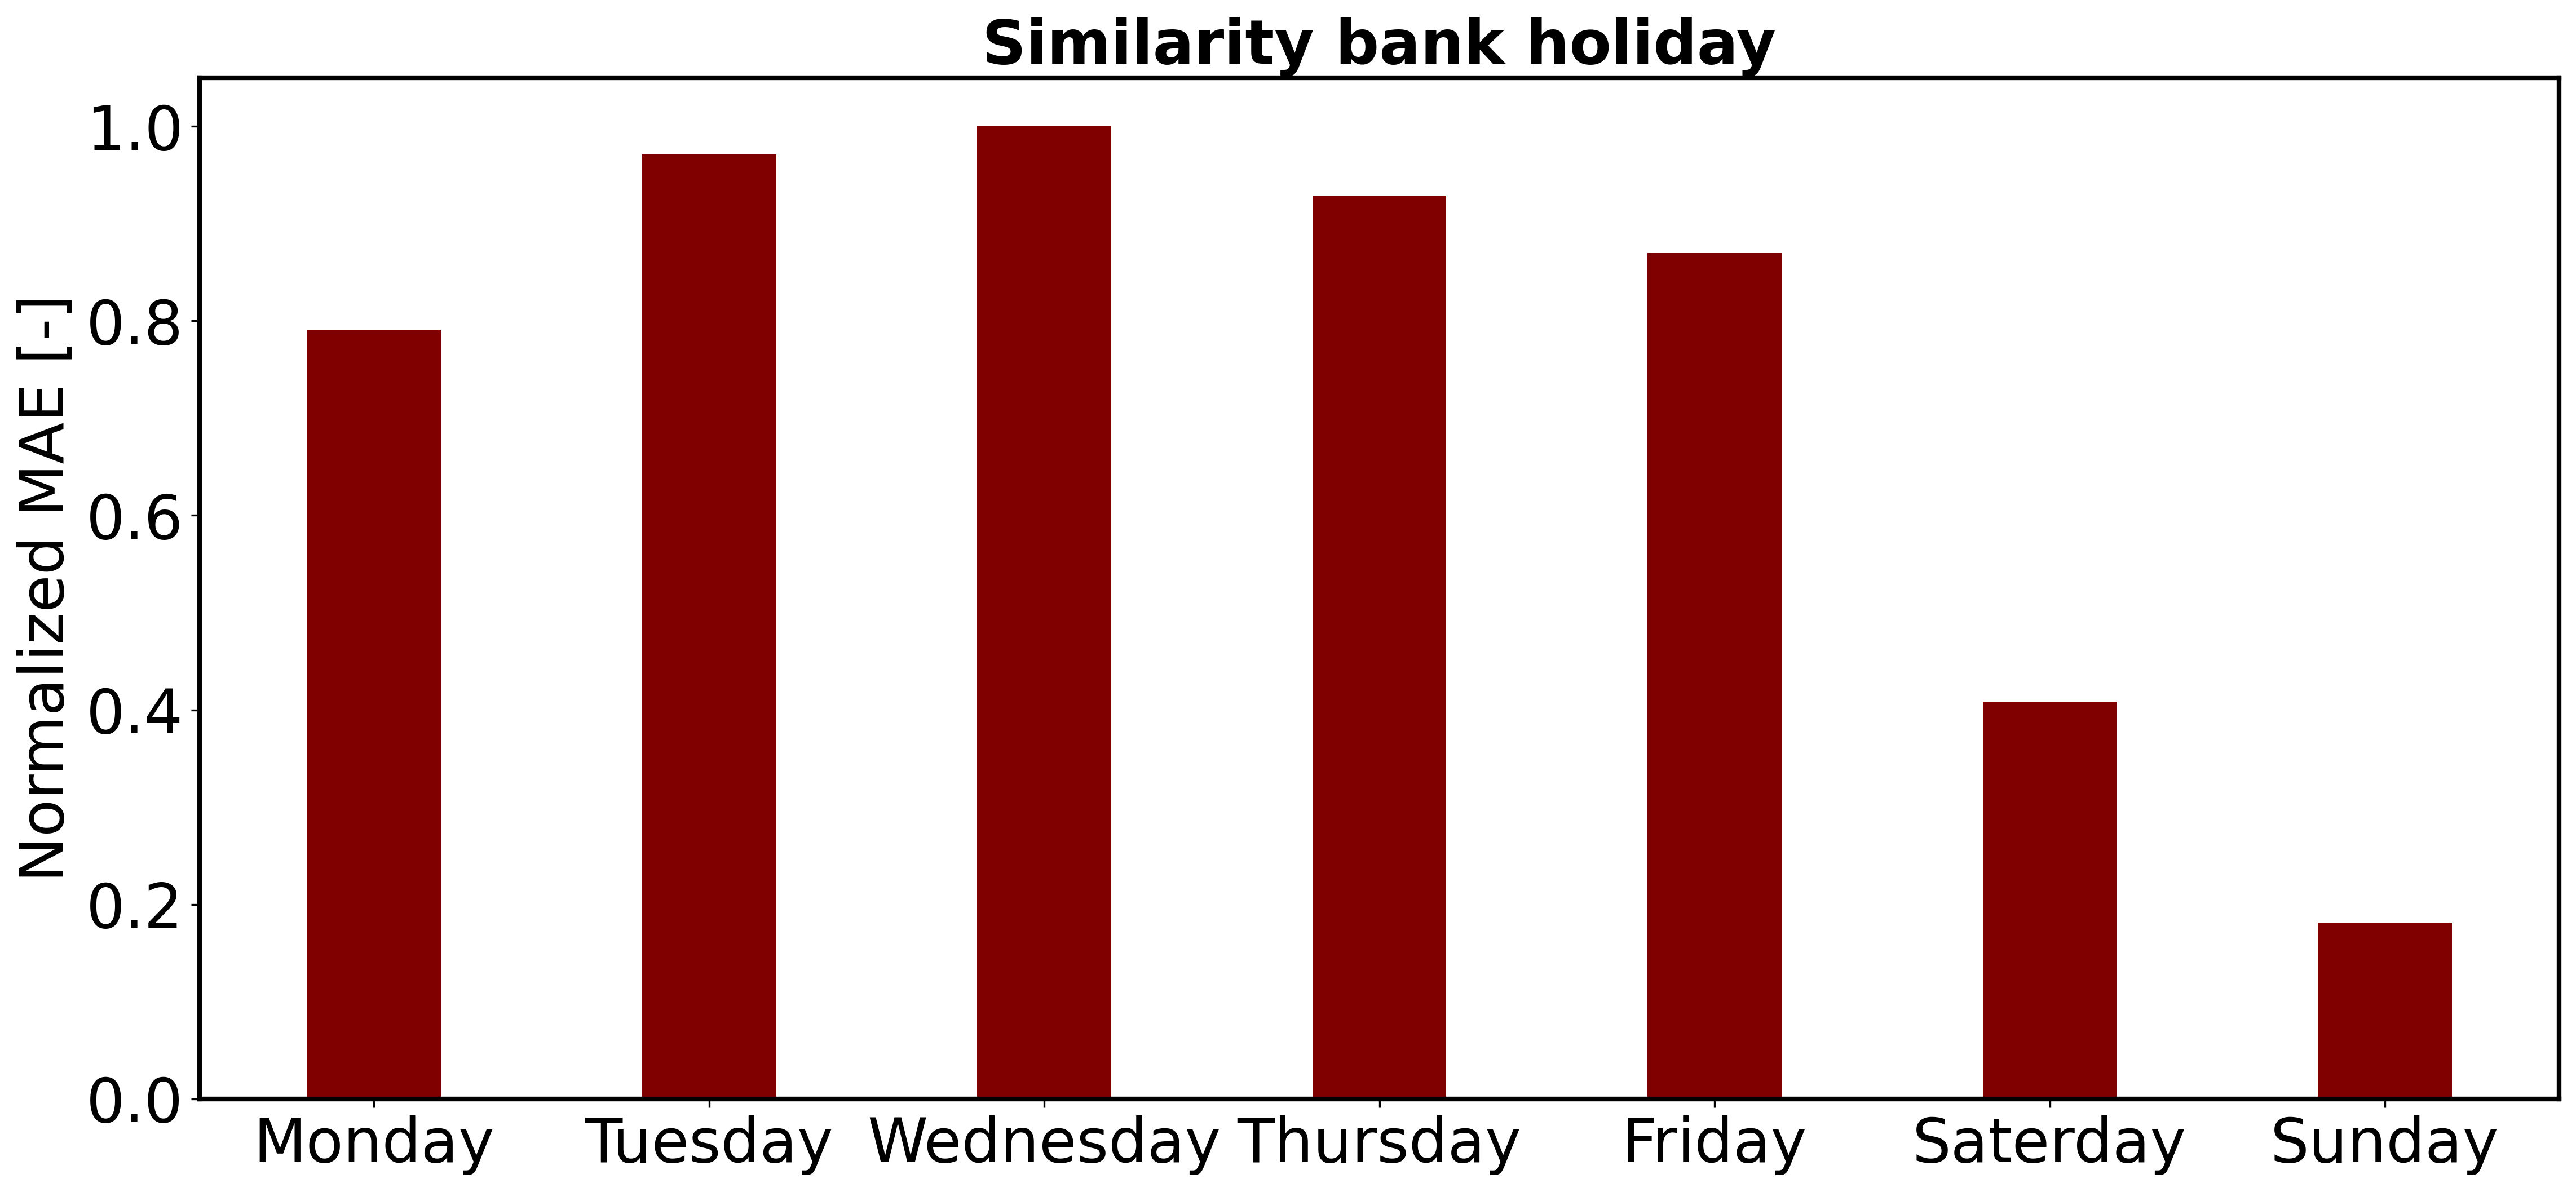
\includegraphics[width=1.0\textwidth]{similarity.png}
	\caption{Error between a bank holiday and other days of the week.}
	\label{fig:sim_weekdays}
\end{figure}


\subsection{Influence of temperature}
% notes on correlation see OneNote.
% use the correlations. https://realpython.com/numpy-scipy-pandas-correlation-python/
% resample the consumption to daily and then apply some of the correlation techniques. 
In this section the correlation between the temperature and the electricity consumption is discussed.\\


\textbf{Pearson correlation}\\
The Pearson correlation is a measure of the linear dependency between two variables, based on the covariance. A Pearson correlation value gives information concerning the magnitude of the association and the corresponding direction of it. A Pearson value of $ 1 $ and $ -1 $ gives respectively a perfect positive and negative linear relation between the variables. A value of zero, corresponds to independent behaviour. The following formula gives the Pearson correlation

\begin{equation}\label{eq:pearson}
	\rho_{X,Y} = \frac{cov(X,Y)}{\sigma_x\sigma_y}.
\end{equation}

Assumptions concerning the Pearson correlation are that samples used for the correlation should be independently drawn, coming in pairs, following homoscedasticity and there are no outliers. Outliers are especially undesirable when there are not a lot of samples. The variables should be normally distributed, linearly related to each other and be continuous. A normal distribution is necessary otherwise the assumption that a distribution can be described by a mean and variance is violated. The samples used for the correlation are generated by calculating the daily consumptions matched with the daily average temperature of the mean signal. Homoscedasticity is important because Eq. \ref{eq:pearson} assumes that $ \sigma_x $ and $ \sigma_y $ are constant values. The homoscedasticity assumption is validated by making use of Figure \ref{fig:pearson}.

\begin{figure}[h!]
	\centering
	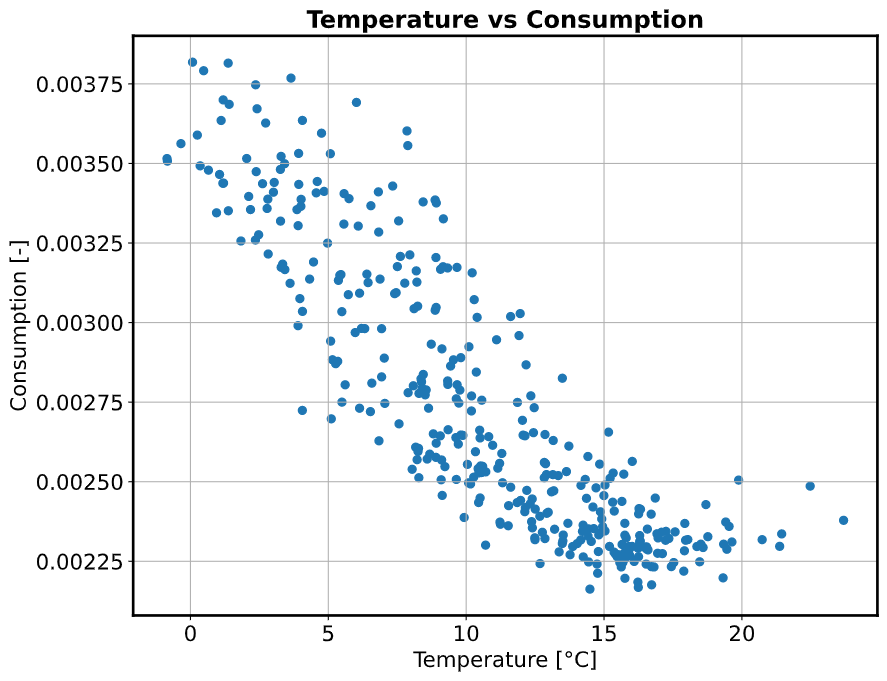
\includegraphics[width=0.8\textwidth]{pearson.png}
	\caption{Relation between normalized daily consumption and daily temperature.}
	\label{fig:pearson}
\end{figure}

This figure shows the classic cone-shaped pattern of heteroscedasticity. On days when it is warm there is more similar human behaviour in lowering the electricity consumption. However, on colder days the variation in consumption is higher, which means that homoscedasticity is not perfectly fulfilled. This is a logical result because when it is cold there can be a lot of variation in what extent electricity is used for heating, while when it is warm everybody is likely to turn of the heating. Because the assumptions of the Pearson correlation are not all met, care should be taken with the output. Applying the Pearson correlation on Figure \ref{fig:pearson} gives a correlation value of $ -0.87 $. This means there is a good linear, decreasing relation.\\


\textbf{Spearman correlation}\\
The Spearman correlation is a rank correlation. A sample consists out of a daily consumption value with a corresponding average temperature value.
The consumption and temperature values belonging to a sample are each compared with respect to all the consumption and temperature values and an ordering is retrieved for both values. When the ordering of both variables in a sample is similar, correlation is strong and positive. If the ordering is reversed, correlation is strong and negative. There is a perfect positive ordering if a larger consumption always corresponds to a higher temperature. Notice that for a perfect ordering, no linear relation of the variables is necessary. The Spearman correlation coefficient is calculated using equation \ref{eq:pearson}, but replaces the values of the variables by the rank of the variables in the a sample.\\

In order to use the Spearman correlation data has to be ordinal, which means that it can be ordered. The Spearman correlation gives information about the monotonicity relation between the variables. $ \rho = 1 $ corresponds to a monotonically increasing relation.\\

Applying the Spearman correlation  gives a correlation value of $ -0.89$, which means there is a large negative monotone relation. This means if the temperature is higher, consumption is likely to be lower and the . Identically, if the temperature is lower it is likely that the consumption will be higher and vice versa. This confirms the conclusions from the Pearson correlation.\\

\textbf{Kendal correlation}\\
The Kendal correlation is also a rank correlation. It is looked how many samples are concordant, discordant or neither when each combination of 2 samples are compared with each other. A concordant pair means that when the consumption value of sample 1 is higher than the consumption value of sample 2, this must also be the case for the temperature values. A discordant pair means that when the consumption value of sample 1 is higher than the consumption value of sample 2, this should be not the case for the temperature. Neither can occur when consumption values or temperature values are equal for the 2 samples. When a Kendal correlation of 1 is retrieved, this means that all samples are concordant and only $ n^+ $ differs from zero. This automatically imposes monotonicity which means that when a consumption value is increased, also the temperature value must be increased. Equation \ref{eq:kendall} gives the equation to calculate the Kendal correlation coefficient. Applying the Kendal correlation  gives a correlation value of $ -0.67$, which again confirms the conclusions from the Pearson correlation.\\

\begin{equation}\label{eq:kendall}
	\tau = \frac{n^+-n^-}{\sqrt{(n^++n^-+n^x)(n^++n^-+n^y)}}
\end{equation}
\begin{itemize}
	\item $ n^+ $ is the number of concordant pairs
	\item $ n^- $ is the number of discordant pairs
	\item $ n^x $ is the number of ties only in x
	\item $ n^y $ is the number of ties only in y
	\item concordant $\rightarrow $ $ (x_i > x_j ) $ and $ (y_i > y_j ) $ or $ (x_i < x_j ) $ and $ (y_i < y_j ) $
	\item discordant $\rightarrow $ $ (x_i > x_j ) $ and $ (y_i < y_j ) $ or $ (x_i < x_j ) $ and $ (y_i > y_j ) $
	\item neither $\rightarrow $ $ (x_i = x_j ) $ or $ (y_i = y_j ) $
	\item if both $ (x_i = x_j ) $ and $ (y_i = y_j ) $ $\rightarrow $ not included in either $ n^x $ or $ n^y $
\end{itemize}



% There is a clear dependency between temperature and electricity consumption, which means that electricity is used for heating.  



\subsection{Identification of driving attributes} \label{s:Identification of driving attributes}
In this section the influence of the extra knowledge about the kind of household where the smart meter is located, is investigated. This is not done by using a single averaged signal as was the case in the previous analysis sections. Now, every meter with additional information is considered. In Figure \ref{fig:bp_dwellingtype} the monthly consumption of the month December in function of dwelling type is shown. The month December is chosen, because this month is known for every smart meter. Missing values of the smart meters are substituted by method two, as discussed in section \ref{s:missing_data}. The amount of meters used for every visualization can be seen in Table \ref{tab:attributes}.

% Boxplots and consumptions are plotted. 

\begin{figure}[h!]
	\centering
	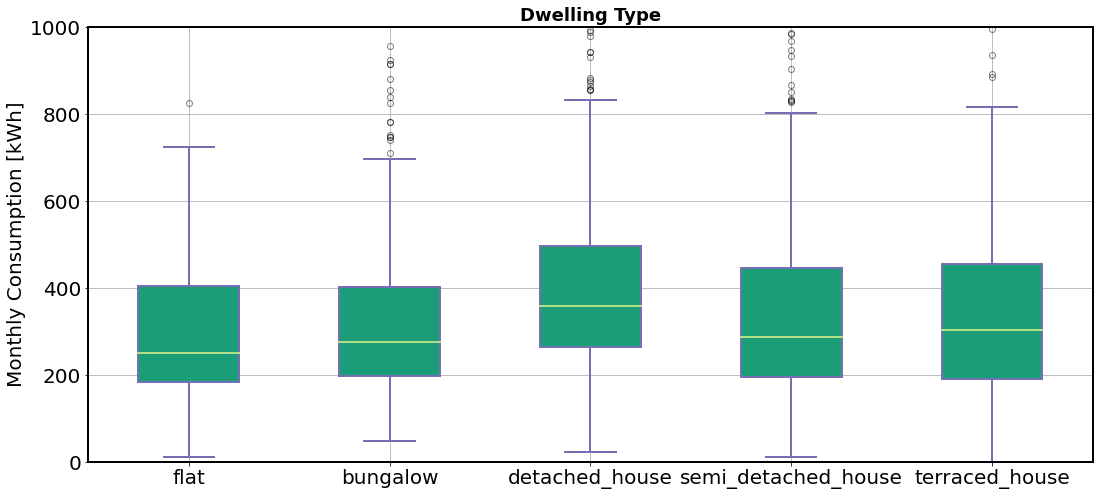
\includegraphics[width=1\textwidth]{bp_dwellingtype.png}
	\caption{Figure with the comparison of the different dwelling types.}
	\label{fig:bp_dwellingtype}
\end{figure}





Similar as was done in Figure \ref{fig:bp_dwellingtype} is also done for the other characteristics of the smart meters. The conclusions are listed below. As can be seen in Table \ref{tab:attributes}, some characteristics have not much data or the data is not much distribute over the different options of a characteristic. If this is the case, no reliable conclusions could be drawn. \textbf{Add concrete numbers!!}

\begin{itemize}
	\item There is a lot of variance in the monthly consumption of a detached house, but it has mostly a higher consumption than other dwelling types
	\item A ``real'' house (detached, semi-detached or terraced) tends to have higher monthly consumptions than a flat or bungalow.  
	\item The order of monthly consumption according to the mean and median values: Flat < Bungalow < Semi-detached < Terraced < Detached
	\item More occupants means more monthly consumption
	\item More rooms in the house means more monthly consumption
	\item Almost all houses use gas as heating fuel
	\item Almost all houses use gas as hot water fuel
	\item The age of the boiler has no clear effect on the monthly consumption
	\item The vast majority of the lofts are insulated
	\item The majority of walls are insulated
	\item The vast majority heats till a temperature between $ 18 $ and $ 20  $ degrees
	\item The majority of people has an efficient lighting percentage between $ 75\% $ and $ 100\% $
	
\end{itemize}



\section{Conclusion}
\textbf{Write a conclusion}
The final section of the chapter gives an overview of the important results
of this chapter. This implies that the introductory chapter and the
concluding chapter don't need a conclusion.




%Please don't abuse enumerations: short enumerations shouldn't use
%``\verb|itemize|'' or ``\texttt{enumerate}'' environments.
%So \emph{never write}: 
%\begin{quote}
%	The Eiffel tower has three floors:
%	\begin{itemize}
%		\item the first one;
%		\item the second one;
%		\item the third one.
%	\end{itemize}
%\end{quote}
%But write:
%\begin{quote}
%	The Eiffel tower has three floors: the first one, the second one, and the
%	third one.
%\end{quote}

%%% Local Variables: 
%%% mode: latex
%%% TeX-master: "thesis"
%%% End: 

\chapter{State of the art short-term residential load forecasting techniques}
\label{cha:State of the art short-term residential load forecasting techniques}
Forecasting the electrical load of the different individual households has a couple of challenges. There should be dealt with the missing values, as discussed in section \ref{s:missing_data}. Also, the different time-series are influenced by exogenous factors as weather conditions and the day of the year. The dependency on exogenous variables can be a very non-linear relation and can have different effects on different households. For example depending on a house has solar panels, the consumption could be altered much. Only three indications of the temperature are given on a daily basis. Some additional information is know of certain households, but this data is very incomplete. Next, the individual load series have a high volatility and uncertainty with respect to a load signal on transmission level which shows more consistent seasonality and straight forward dependency on weather and calendar variables. This is because the contingency of the individual load data is mitigated due to averaging out of the uncertainty. Ofcourse, the obvious disadvantage is that only forecasts on this aggregated level can be made which is not the goal of our investigation.\\ To tackle the high non-linearity that is inherent to residential load forecasting in literature often ``Neural Networks'' are used.
\textbf{See also paper TA2 --> aggregated vs individual forecasting.}

\section{Introduction to Neural Networks}
A  standard multilayer feedforward neuralnetwork with locally bounded piecewise continuous activation function can approximate any continuous function to any degree of accuracy if and only if the network's activation function is not a polynomial, as stated by \textbf{Leshno et al} in \textbf{1993}. This theorem proofs that a ``universal approximator'' exists for continuous functions, but it lacks the recipe to construct it. In \cite{Nielsen2015} it is shown that a feedforward network with a single layer is enough to approximate any function by a specified accuracy if the hidden layer has the possibility to add an unlimited amount of hidden neurons in its layer. It is discussed that when a function is discontinuous, which means that it makes sudden, sharps jumps, it is not possible to approximate the function by any prescribed accuracy. However, in practise a continuous approximation is often good enough.\\

Neural networks are suitable of learning very non-linear mappings between inputs and outputs. The difference between ``Deep Neural Networks'' and ``Shallow Neural Networks'' is the amount of layers of neurons are used inside the network. These layers of neurons, that are not inputs or outputs are called ``hidden neurons''. Because a ``Deep Neural Network'' has a hierarchical layout of the different hidden layers, it not only learning features from the non-linear combinations of inputs, but uses other layers to learn features of combinations of features learned in lower hidden layers. This is possible because higher hidden layers get the outputs of lower hidden layers as input. As discussed in  \cite{Shi2018} due to this characteristic, deep learning is suitable to learn multiple uncertainties with differing sharing levels over different households e.g. the amount of sunshine. However, because of the higher expressiveness (and often the amount of the to learn parameters), a ``Deep Neural Network'' with respect to a ``Shallow Neural Network'', suffers more of overfitting as is discussed in section \ref{s:Problems}.

\subsection{MLP}
The simples configuration of deep networks are multilayer perceptrons and they are made up out of multiple fully connected layers of neurons. Figure \ref{fig:MLP} shows a MLP with one hidden layer.

\begin{figure}[h!]
	\centering
	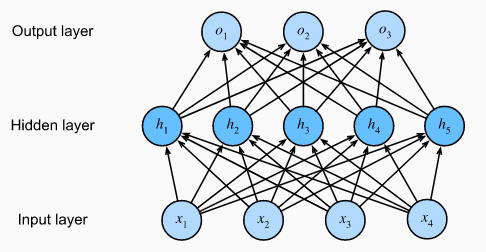
\includegraphics[width=0.8\textwidth]{MLP.png}
	\caption{Figure of a MLP (source \cite{Czum2020}).}
	\label{fig:MLP}
\end{figure}

All layers are connected to the next layer by the means of an affine function together with a non-linear activation function represented by sigma as shown by equation \ref{eq:NN} with $ \textbf{L}^{(N)} $ the vector with outputs of the Nthe layer, $ \textbf{W}^(N) $ the Nth weight matrix and $ \textbf{b}^{(N)} $ the Nth bias. 

%It can be noted that the MLP network is invariant.

\begin{equation}\label{eq:NN}
	\textbf{L}^{N+1} = \sigma(\textbf{W}^{(N)}\textbf{L}^{N}+\textbf{b}^{(N)})
\end{equation}


\subsection{CNN}
\textbf{See oneNote}

\subsection{RNN}
A recurrent Neural Network is a specialized neural network to better deal with sequential information. While traditional deep neural networks assume that inputs and outputs are independent of each other, the output of recurrent neural networks depend on the prior elements within the sequence. In order to take past information from previous inputs into account, a hidden variable $ h_t $ is used. By making use of this variable which makes a summary of the previous seen information, an exponential increase in the number of model parameters is avoided. Equation \ref{eq:RNN} shows how the previous hidden state and the current information are merged in the next hidden state with $ \textbf{X}^t\in \mathbb{R}^{d\times 1} $, $ \textbf{H}^t\in \mathbb{R}^{h\times 1} $, $ \textbf{W}_1\in \mathbb{R}^{h\times d} $, $\textbf{W}_2\in \mathbb{R}^{h\times h} $ and $ \textbf{b}\in \mathbb{R}^{h\times 1} $. 

\begin{equation}\label{eq:RNN}
	\textbf{H}^{t+1} = \sigma(\textbf{W}_1\textbf{X}^{t}+\textbf{W}_2\textbf{H}^{t}+\textbf{b})
\end{equation}

The equation $\textbf{X}^t$ corresponds to one example at time step $ t $ with dimensionality $ d $. 
Also a deep RNN is possible, where multiple hidden state per time step are used. \\

%The mapping from the hidden state to an output is executed by making use of Equation \ref{eq:RNNout} with $ \textbf{O}^t\in \mathbb{R}^{q\times 1} $, $ \textbf{H}^t\in \mathbb{R}^{h\times 1} $, $ \textbf{W}_3\in \mathbb{R}^{q\times h} $ and $ \textbf{b}\in \mathbb{R}^{q\times 1} $.
%\begin{equation}\label{eq:RNNout}
%	\textbf{O}^{t} = \textbf{W}_3\textbf{H}^{t}+\textbf{b}
%\end{equation}


\begin{figure}[h!]
	\centering
	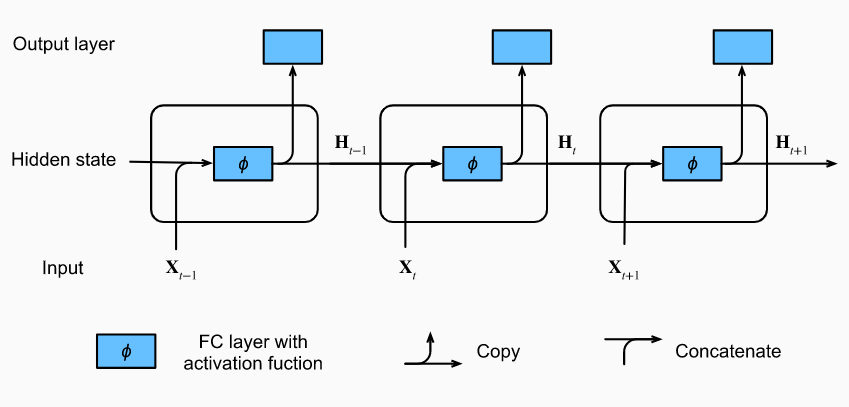
\includegraphics[width=1.0\textwidth]{RNN.png}
	\caption{Figure of the logical flow of a vanilla RNN with a hidden state (source \cite{Czum2020}).}
	\label{fig:RNN}
\end{figure}




\subsection{Difficulties \& Solutions of neural networks}\label{s:Problems}
Neural Networks have a high expressiveness but comes at the cost of overfitting and a vanishing gradient.
when the NN is learning from training data, every epoch the error between the input and output of the training exemples is reduced. In the beginning the generalization error reduces simultaneously with the generalization error. The generalization error is the error that the model makes on data that is not in the training set. However, on a certain point during the training the generalization error increases while the training error still decreases. This means that the model is no longer learning ``intelligent'' general rules and patterns in the data, but is just remembering the training data and will therefore not apply in general. This is often the case in a model with high expressiveness because the model is less pushed to make generalizations and has the ability to just to remember the training data. Solutions to overfitting can be regularization which includes the parameter norms as a cost in the objective function. Typical choices for resembling the size of a parameter are the $ L_1 $ and the $ L_2 $ norms. Other methods that can be used are: early stopping, dropout and pruning.

It should also be noted that the gradient can increase very much, which in literature is called gradient explosion. The solution strategy for this is applying gradient clipping.\\

The second problem is the vanishing gradient problem which originates because while using the backpropagation algorithm to calculate the gradient which is used in different update methods of the weights, the gradient is calculated at the end of the NN and propagated back using every time the previous calculated gradient values who exponentially decrease. Therefore at the first layers of the network, the gradient has become so small that the weights are almost not updated anymore. In a RNN setting this corresponds to having a short term memory which means that initial inputs that were presented to the NN are being forgotten. Mitigation strategies often proposed in literature are LSTM and GRU. Both techniques have in common that they can learn which data in the sequence is important and should be retained and which information can be thrown away. It is important to state that LSTM and GRU are not solving the vanishing gradient problem as explained in \cite{Teuwen2019}. The gradient is still exponentially decreasing, but the effect is less pronounced as can be seen for LSTM in Figure \ref{fig:grad_exp}. $ \tau $ gives the number of epochs.\\ \textbf{Can put further explanation in attachment --> see assignament ANN}

\begin{figure}[h!]
	\centering
	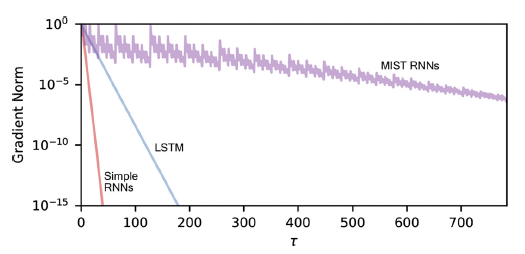
\includegraphics[width=0.8\textwidth]{grad_exp.png}
	\caption{Exponential decrease of the gradient size of a simple RNN (red) or a LSTM (blue) (source \cite{Teuwen2019}).}
	\label{fig:grad_exp}
\end{figure}


\textbf{LSTM}\\
Next, a LSTM (long short term memory) neural network will be assessed to model the Santa Fe data set instead of the MLP regression neural network that was used in the previous section . A LSTM has as advantage over a standard RNN that I can better handle the vanishing gradient problem and LSTM is not suffering as much of a short term memory. Therefore, it can  longer take important aspects of the presented time-serie into account when working on a new forecasting. LSTM makes use of three gates to learn which data of the sequence is important and should be remembered. In connection of these gates is a cell state which serves as a memory state and a connection to transport relative information throughout the different time steps. The forget gate decides what information should be kept or removed from the input and hidden state. The input gate updates the cell state and the output state decides what the next hidden state will be.\\
In order to train a LSTM neural network there are more parameters that have to be learned.  There are now four different weight matrices. One form the forget gate, two from the input gate and one from the output gate. It can be noted that in order to train all these weights, this network is more data hungry than a simple RNN. When the lag value gets bigger, so do all the different weight matrices and the calculation load.\\

 



%\textbf{Vanishing gradient}\\
%LTSM --> vanishing gradient problem is not solved! Mittigated. 
%GRU
%Attention model
%Transer model


\section{Short-Term residential electrical load forecasting}
\textbf{Pooling paper}
%Things should get out of paper:
%Problem that was solved.
%Method
%Result
Classical ways to deal with uncertainty.\\
Residential electrical load series have a high amount of volatility and uncertainty due to the contingency of the electrical consumption. Classical ways to deal with this are discussed in \cite{Shi2018} and listed as follows:
\begin{enumerate}
	\item Clustering to group similar houses based on historic load or exogenous consumption driving variables. Because the load or driving variables are similar in a cluster, the variance of uncertainty is also decreased. However, performance is very dependent of the dataset. \textbf{But the uncertainty on the whole is reduced --> on single household stays the same!!}
	\item Aggregating the residential loads to cancel out the uncertainties. The aggregated signal will show more regular patterns which means that is easier to predict.The downside is that the aggregated forecast will do a poor job of serving as forecast for a household
	\item A spectral analysis e.g. wavelet analysis, Fourier transforms and empirical mode decomposition aim at seperating a load serie into a regular pattern, an uncertain signal and noise. Because the amount of regularity is low in a residential load serie, this method is infeasible.
\end{enumerate}



In this paper \cite{Shi2018} a novel pooling-based deep recurrent neural network is proposed which collects load profiles of neighbouring houses into a pool of training inputs. Pooling of neighbouring households historical loads to serve as input of the ``Deep Recurrent Neural Network'', is proposed to increase the data volume and diversity of load forecasting, which mitigates the effect of overfitting present in a DRNN. The idea is as quoted by \cite{Shi2018} to use the interconnected spacial information to compensate insufficient temporal information.Thereby, the pool of data allows to learn the correlations between neighbouring households and the shared uncertainties coming from external factors e.g. temperature.  Also, due to the pooling of different households during training the DRNN is able to learn common uncertainties. In paper \cite{Shi2018} pools consisting of $ 10 $ households are used. From the pool of inputs every epoch a randomly chosen batch of load signals are fed to the network. LSTM is applied to mittigate the short term memory of the RNN. Additionally, there is been made use of early stopping to further avoid overfitting. To implement early stopping there has been looked at the ``MSE'' for k iterations, obtained by cross-validation. When the variance of this sequence gets smaller than a specified variable, training stops. When the training ends, performance is tested on each household by using the learned network to perform a feed-forward prediction of the electrical load.\\

An overview of the different steps that were done during the proposed method are: data cleaning and preprocessing $\rightarrow$ data pooling $\rightarrow$ data sampling $\rightarrow$ data training $\rightarrow$ benchmarking.\\

Performance of the proposed method was finally evaluated based on a test set of the last $ 30 $ days and consisting out of : 
\begin{enumerate}
	\item performance of the proposed method with respect to Vanilla RNN, SVR and DRNN (without pooling)
	\item the effect of the neural network depth and pooling
\end{enumerate}

The proposed DRNN with pooling outperforms all other four methods based on following three metrics:

\begin{equation}
	RMSE = \sqrt{\frac{\sum_{t=1}^{N}(\hat{y}_t-y_t)^2}{N}}
\end{equation}
\begin{equation}
	NRMSE = \frac{RMSE}{y_{max}-y_{min}}
\end{equation}
\begin{equation}
	MAE = \frac{\sum_{t=1}^{N}\abs{\hat{y}_t-y_t}}{N}
\end{equation}
\textbf{Actually LSTM network}
The amount of which the PDRNN outperformed the other methods can be seen in Table \ref{tab:pooling_result}. The effect of the depth of the DRNN and the pooling method is depicted in Figure \ref{fig:Shi2018_result}. It can be seen that without the pooling method the DRNN only benefits from extra layers till three are used. This is because from that point, overfitting will reduce the generalization capacity of the DRNN. With the pooling technique, extra layers stays beneficial. It can thus be concluded that introducing extra hidden layers is a good choice to model the non-linear relations, but this can only be done efficiently when overfitting is mittigated by the use of a pooling strategy.The RNN with pooling used for benchmarking consisted out of five layers and thirty hidden units in each layer.

\begin{figure}[h!]
	\centering
	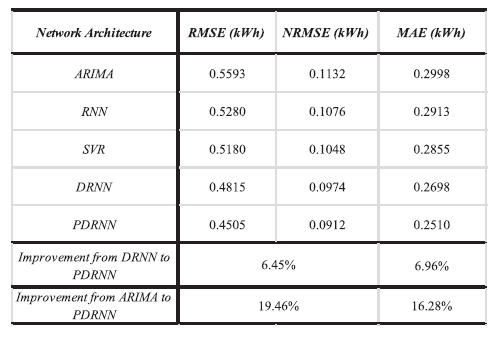
\includegraphics[width=1\textwidth]{pooling_result.png}
	\caption{Results obtained in paper \cite{Shi2018} using the PDRNN method.}
	\label{fig:Shi2018_result}
\end{figure}

\begin{figure}[h!]
	\centering
	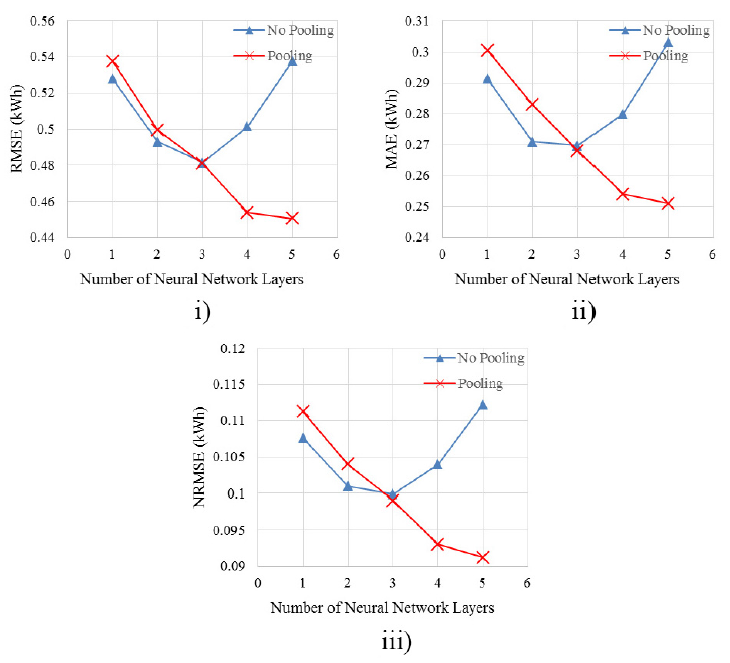
\includegraphics[width=1\textwidth]{Shi2018_result.png}
	\caption{Influence of the number of layers and the pooling method used in \cite{Shi2018}.}
	\label{fig:Shi2018_result}
\end{figure}

GRU (Gated Reset Update) or LSTM (Long Short Term Memory) can be implemented. They are both enhancements of the vanilla RNN which suffers from a vanishing gradient which causes it to to behave without a long term memory. In practise to know which one works often both are tried \cite{Teuwen2019}. Stochastic gradient descent means that the approximated gradient is calculated from a random subset of the available data instead from the entire dataset. \\

\textbf{Short-term Residential load forecasting based on LSTM RNN paper}\\
In \cite{Kong2019} it is chosen for a LSTM approach to forecast the complex temporal consumption pattern which characterises a single household electricity load. It is discussed that the diversity in the aggregated level of the individual electrical loads, smooths the daily load profile. This has as effect that the aggregated electrical load time-serie becomes more predictable, while a single household electrical load is more dependent on the human behaviour of its residents. This is substantiated by making use of a density based clustering technique where it was shown that the different daily consumptions of the aggregated signal could be described by one cluster and no outliers. An outlier means that a daily consumption could not be assigned to a cluster. On the other hand for individual time series the amount of outliers could range to over $ 80 $. To compare the consistency of different individual load signals the amount of outliers could therefore be used.\\
Because the residents daily routine is characterizing the household load so much, this is tried to be learned directly inside the LSTM RNN.\\
Inputs that are given to the LSTM are k past half hour load measurements, the time of when this measurements were taken, the day of the week of the measurements and if this day is a holiday or not. In table \ref{tab:LSTM_lit_result} the results are shown of the LSTM RNN method in comparison with other forecasting techniques. It can be noted that the proposed technique outperforms the rest based on the average performance of $ 29,808 $ individual forecasts of half an hour individual loads. Forecasting was performed on $ 69 $ different electrical loads coming from households in Australia.  However, for individual load series forecasting the MAPE minimization is also remarkable when considering its simplicity in comparison with LSTM. Next, it was concluded that learning methods that had good performance on aggregated time-series e.g. IS-HF and KNN, perform much worse when predicting individual loads. \\
Further, by making use of a regresion technique in function of the amount of outliers it is shown that LSTM and BPNN (Back-Propagation Neural Network) perform similar for, as previously discussed, consistent individual loads. The LSTM only starts to differentiate in performance when inconsistency grows. To conclude things that lack in \cite{Kong2019} are practical useful forecasts of a timespan of $ 24 $h instead of only half an hour and making use of a rule of thumb when parameter tuning. Hyperparameters that can be tuned in LSTM are: learning rate, lag variable, amount of hidden layers and the amount of hidden nodes.\\

\begin{figure}[h!]
	\centering
	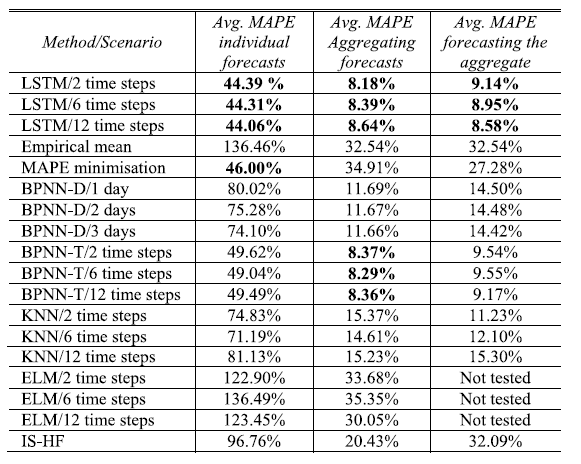
\includegraphics[width=1\textwidth]{prev_appr.png}
	\caption{Different approaches tried in \cite{Kong2019} and their averaged performance of $ 29,808 $ individual forecasts of half an hour individual loads. }
	\label{tab:LSTM_lit_result}
\end{figure}

\textbf{CNN-LSTM paper}\\
In \cite{Kim2019} a novel technique is proposed which makes use of a convolutional neural network from which the outputs are given to a LSTM recurrent network after which a fully connected neural network  is used to produce the outputs. The purpose of the CNN is to extract the features that are the main drivers of energy consumption and to remove the noise that comes initially together with the raw inputs. The CNN is made up out of convolution layers and pooling layers and makes use of the ``ReLU'' activation function. The main purpose of a convolution layer is to extract features while the pooling layer reduces the number of parameters by making use of the ``max pooling principle''. Using the ``max pooling principle'' means taking the max value of each neuron cluster of the previous layer. As discussed in paper \cite{Kong2019} LSTM is suitable to alleviate the problem of a vanishing or exploding gradient which characterized a simple RNN. LSTM is able to preserve long-term memory by making use of memory states that is used in the calculation of hidden states. It is therefore suitable to remembering the irregular trend of the electrical load time-serie. Finally, a fully connected time-serie predicts the load forecast.\\
Paper \cite{Kim2019} further showed superiority with respect to only making use of the LSTM layers as can be seen in Table \ref{tab:CNN-LSTM_results}. The  Inputs that were used to forecast the household load which is located in France are: three submeters with historical loads, global intensity, voltage, global reactive power, global active power, time, data and month. 
At last, also an analysis is performed to investigate the influence of the different inputs by calculating the average class activation score over the inputs. The results are shown in Figure \ref{fig:LSTM-CNN_results}. It can be seen that especially ``Sub metering $ 3 $'' has a big influence on the final forecasts. This sub meter corresponds to the the electric water heater and air conditioner of the house. As was shown in Section \ref{tab:attributes} the dataset used in this thesis gives only information about the presence of a hot water heater.  Discussed limitations in the paper are the definition of the hyper parameters that were set by trail and error instead of using an automated method e.g. a genetic algorithm. A further limitation is the lack of household characteristics e.g. the amount of residents living in the house. It has previously been shown by \textbf{C. Beckel et al.} that household occupancy is one of the primarily drivers of electrical consumption in a household.\\

\begin{figure}[h!]
	\centering
	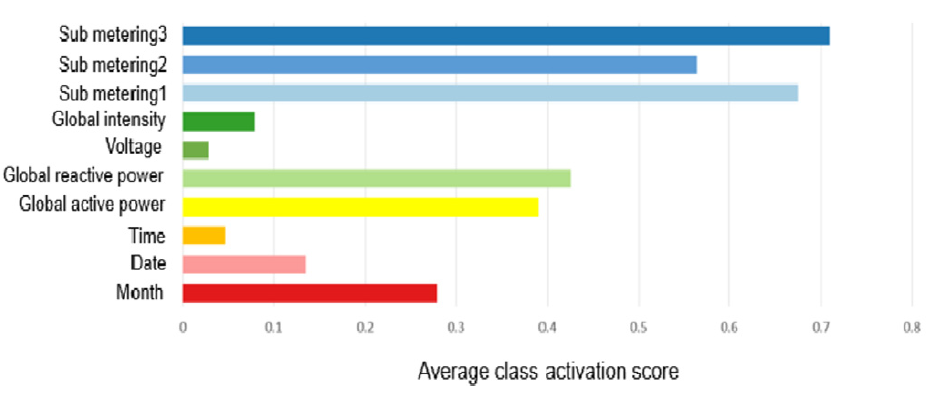
\includegraphics[width=1\textwidth]{CNN-LSTM_results_F.png}
	\caption{The importance of the different inputs as based on the average class activation score. (source \cite{Kim2019})}
	\label{tab:LSTM_lit_results}
\end{figure}

\begin{figure}[h!]
	\centering
	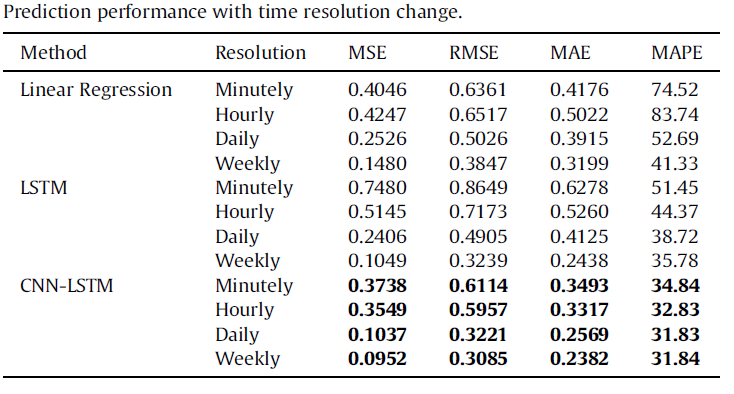
\includegraphics[width=1\textwidth]{CNN-LSTM_results_T.png}
	\caption{Comparison between LSTM and CNN-LSTM. source(\cite{Kim2019})}
	\label{tab:LSTM_lit_results}
\end{figure}

\textbf{CNN-GRU paper}\\
\cite{Sajjad2020}







\section{Tables}
Tables are used to present data neatly arranged. A table is normally
not a spreadsheet! Compare \tref{tab:wrong} en \tref{tab:ok}: which table do
you prefer?

%\begin{table}
%  \centering
%  \begin{tabular}{||l|lr||} \hline
%    gnats     & gram      & \$13.65 \\ \cline{2-3}
%              & each      & .01 \\ \hline
%    gnu       & stuffed   & 92.50 \\ \cline{1-1} \cline{3-3}
%    emu       &           & 33.33 \\ \hline
%    armadillo & frozen    & 8.99 \\ \hline
%  \end{tabular}
%  \caption{A table with the wrong layout.}
%  \label{tab:wrong}
%\end{table}
%
%\begin{table}
%  \centering
%  \begin{tabular}{@{}llr@{}} \toprule
%    \multicolumn{2}{c}{Item} \\ \cmidrule(r){1-2}
%    Animal    & Description & Price (\$)\\ \midrule
%    Gnat      & per gram    & 13.65 \\
%              & each        & 0.01 \\
%    Gnu       & stuffed     & 92.50 \\
%    Emu       & stuffed     & 33.33 \\
%    Armadillo & frozen      & 8.99 \\ \bottomrule
%  \end{tabular}
%  \caption{A table with the correct layout.}
%  \label{tab:ok}
%\end{table}



\section{Conclusion}
The final section of the chapter gives an overview of the important results
of this chapter. This implies that the introductory chapter and the
concluding chapter don't need a conclusion.



%%% Local Variables: 
%%% mode: latex
%%% TeX-master: "thesis"
%%% End: 

\chapter{Clustering of the load profiles}
\label{cha:n}
Do a literature study about forecasting. What is the current state of the art methods to do forecasting. 

\section{The First Topic of this Chapter}
\subsection{Item 1}
\subsubsection{Sub-item 1}
\lipsum[80]

\subsubsection{Sub-item 2}
\lipsum[81]

\subsection{Item 2}
\lipsum[82]

\section{The Second Topic}
\lipsum[83-85]

\section{Conclusion}
\lipsum[86-88]

%%% Local Variables: 
%%% mode: latex
%%% TeX-master: "thesis"
%%% End: 

\chapter{Model evaluation}
\label{cha:Model evaluation}

This chapter discusses the performance of the models that were introduced in Chapter \ref{cha:Forecasting the daily electricity consumption} on the test set. As was shown in Table \ref{tab:summ_data}, the test set consists out of the days of the month December. The goal of the test set is to assess the model performance on new data and it is therefore important that the models are not trained and their parameters are not tuned using this data. Missing days in the test set are removed to avoid the influence of the estimation error of the reference signal on the model performance. In this chapter first the model selection is explained after which a discussion of the performance on the test set follows.

\section{Model selection}\label{s:Model selection}
In Chapter \ref{cha:Forecasting the daily electricity consumption} the model parameters are tuned, but there is still a factor of random model performance due to the random initialization of the weight matrices. To reduce this influence, the model is trained $ 10 $ times and the model that performed best on a validation set using the $ MAE $ metric is selected. As validation set the $ 10 $ last days of November are used. Also, during training early stopping is applied wherefore an additional $ 10\% $ of the training data is taken to serve as a second validation set. For a stateless model this $ 10\% $ is randomly taken from the remaining training data. For a stateful model this $ 10\% $ originates form the end of the training data. The patience parameter is taken as $ 5 $, which means that the validation error can increase $ 5 $ times before the model is stopped. The maximum amount of epochs that is allowed is set to $ 150 $. The parameter values obtained after tuning for the three time series can be found in Chapter \ref{cha:Forecasting the daily electricity consumption}. Table \ref{tab:summ_model_selection} summarizes the amount of epochs that the selected model ran. There can be a large difference in the amount of training epoch and Table \ref{tab:summ_model_selection} shows that Serie 2 needs often a lot of epochs. Although, it was found that for both Model 2 and 3 there is not much improvement anymore on the training and validation sets after respectively epoch $ 60 $ and epoch $ 20 $ as shown in Figure \ref{fig:training_validation}. Model 3 takes longer to predict than the other two models due to the additional seeding that is required.

\begin{table}[h]
	\centering
	\begin{tabular}{@{}l|ccc@{}} \toprule
				         & \textbf{Model $ 1 $} & \textbf{Model $ 2 $} & \textbf{Model $ 3 $}\\\midrule
		\textbf{Serie 1} & $5 $&$ 16$  & $5 $\\
		\textbf{Serie 2} & $7 $&$ 150 $  & $150$\\
		\textbf{Serie 3} & $19 $&$ 11 $  & $6$\\\bottomrule
	\end{tabular}
	\caption{The amount of training epochs for each selected model.}
	\label{tab:summ_model_selection}
\end{table}

\begin{figure}	 	
	\centering
	\begin{subfigure}{0.49\textwidth}
	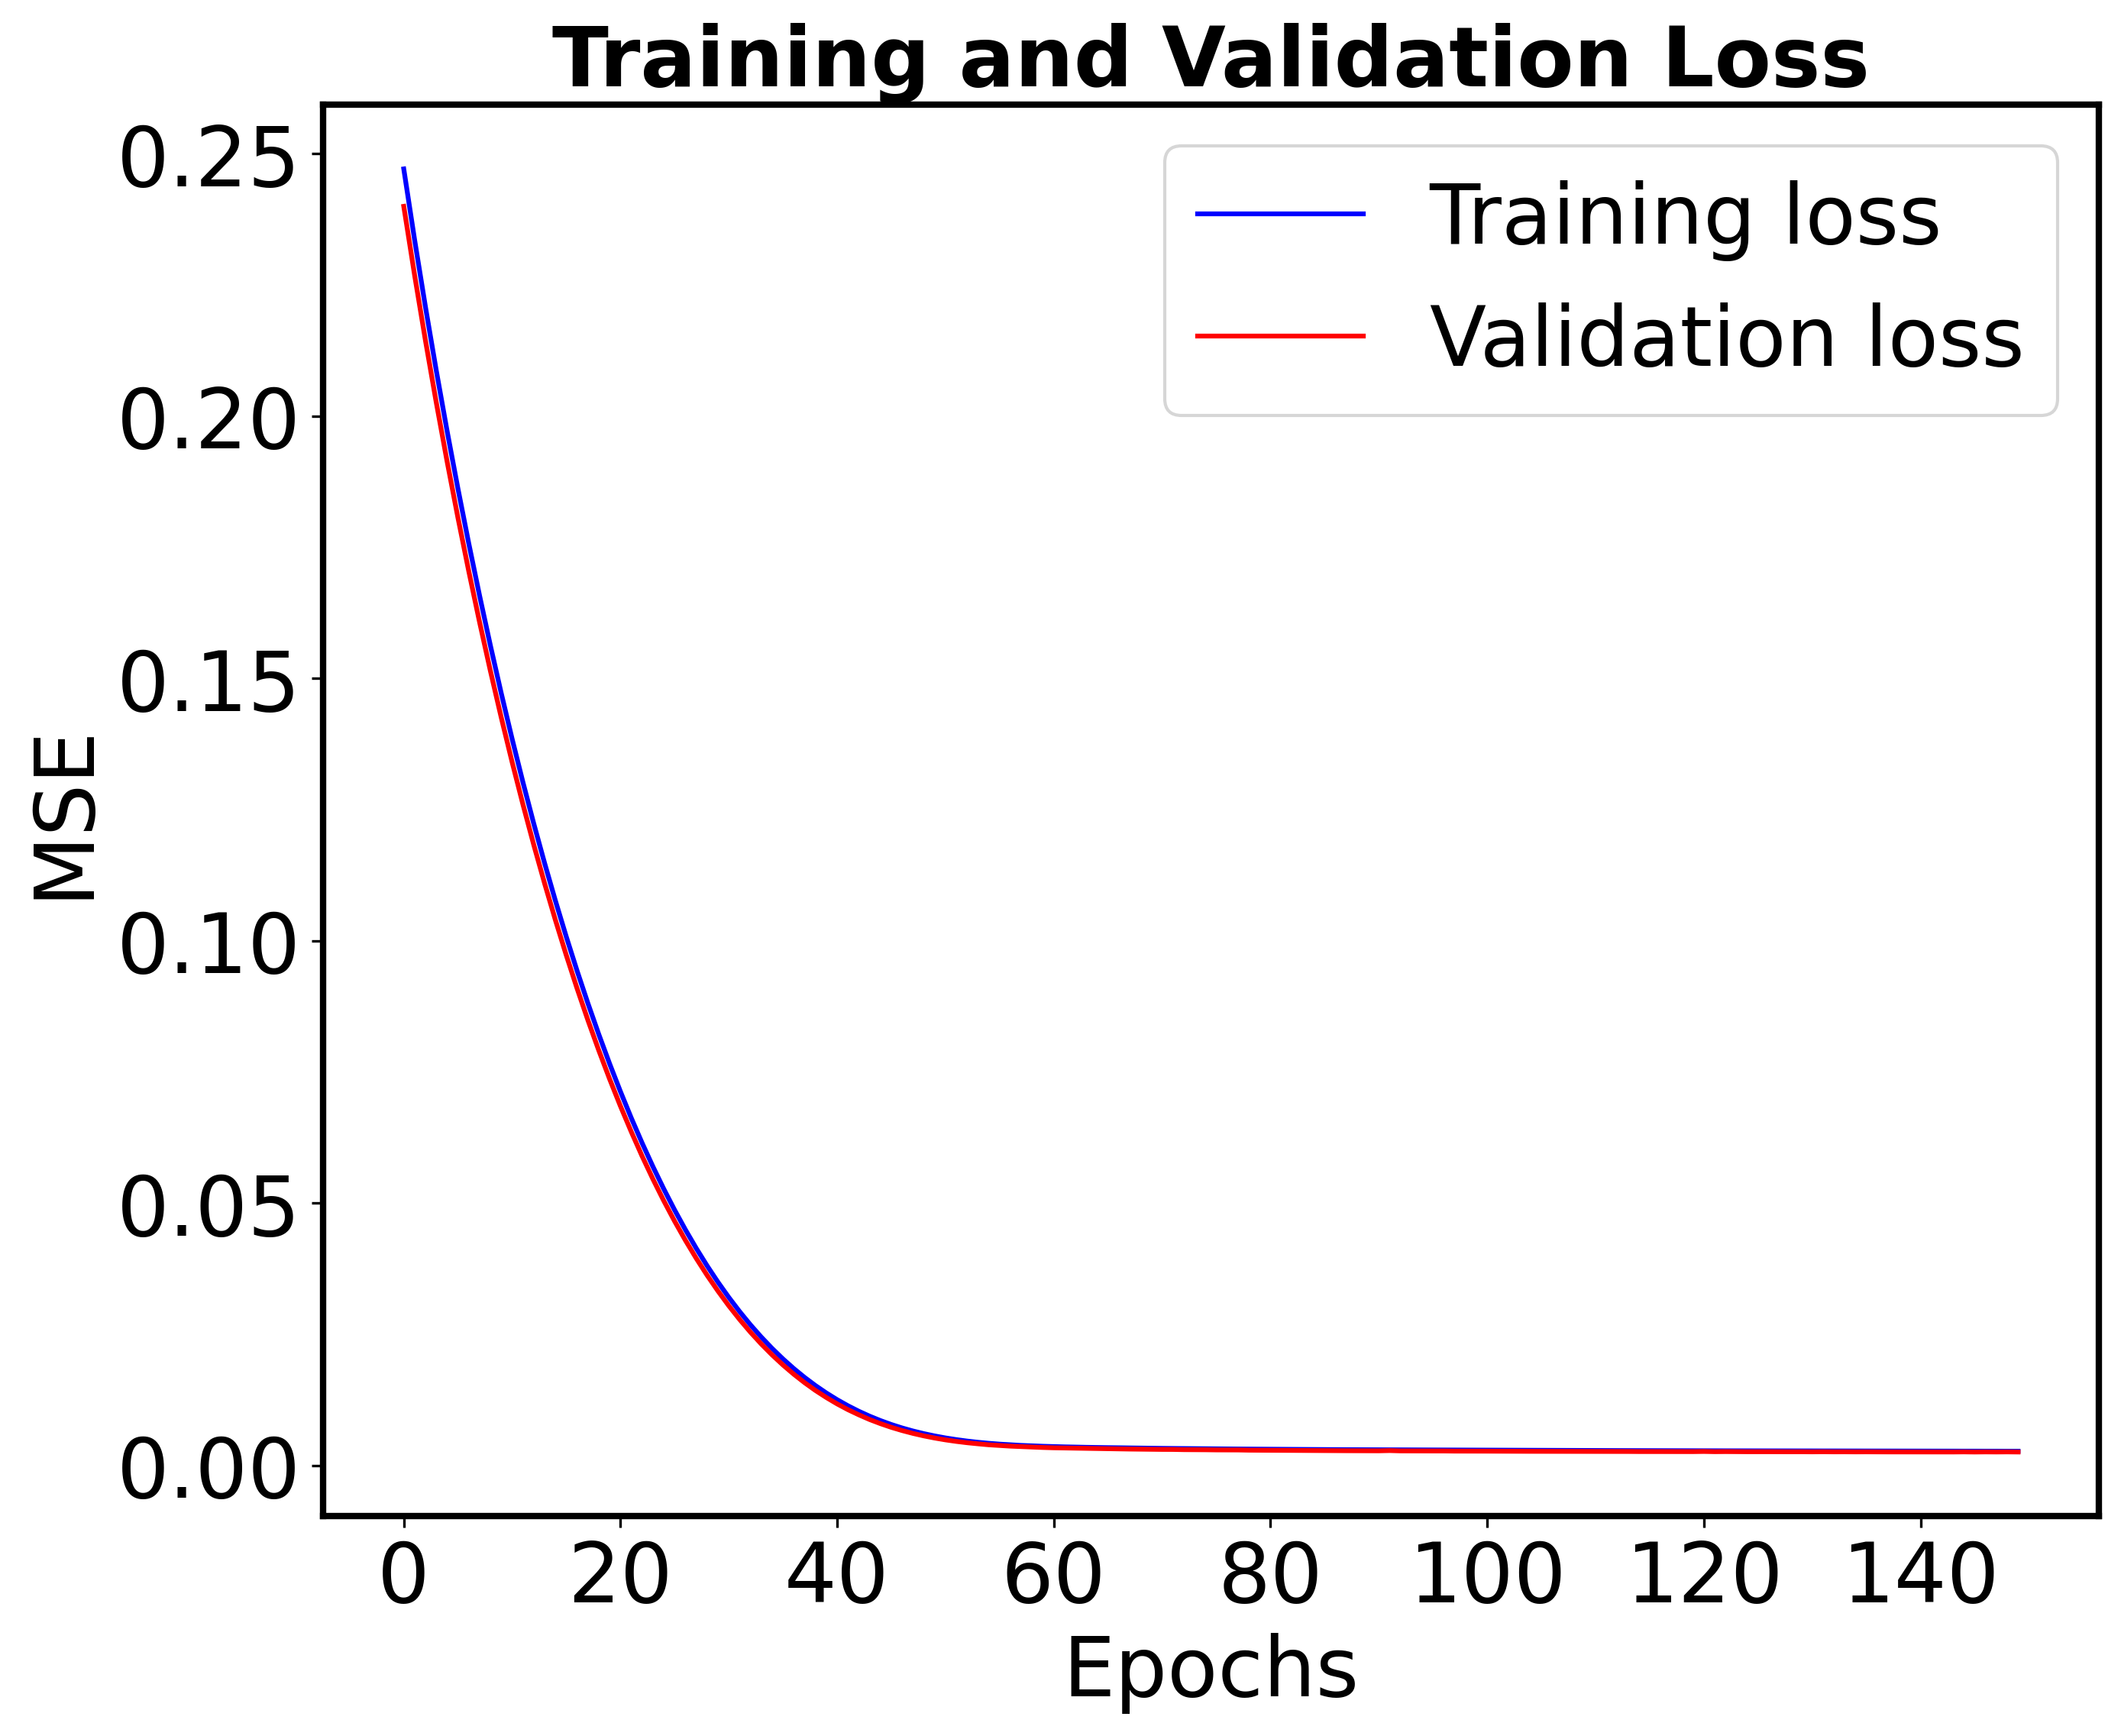
\includegraphics[width=1\linewidth]{Model2_Serie2.png}
	\caption{Model 2 - Serie 2}
	\end{subfigure}	
	\begin{subfigure}{0.49\textwidth}
	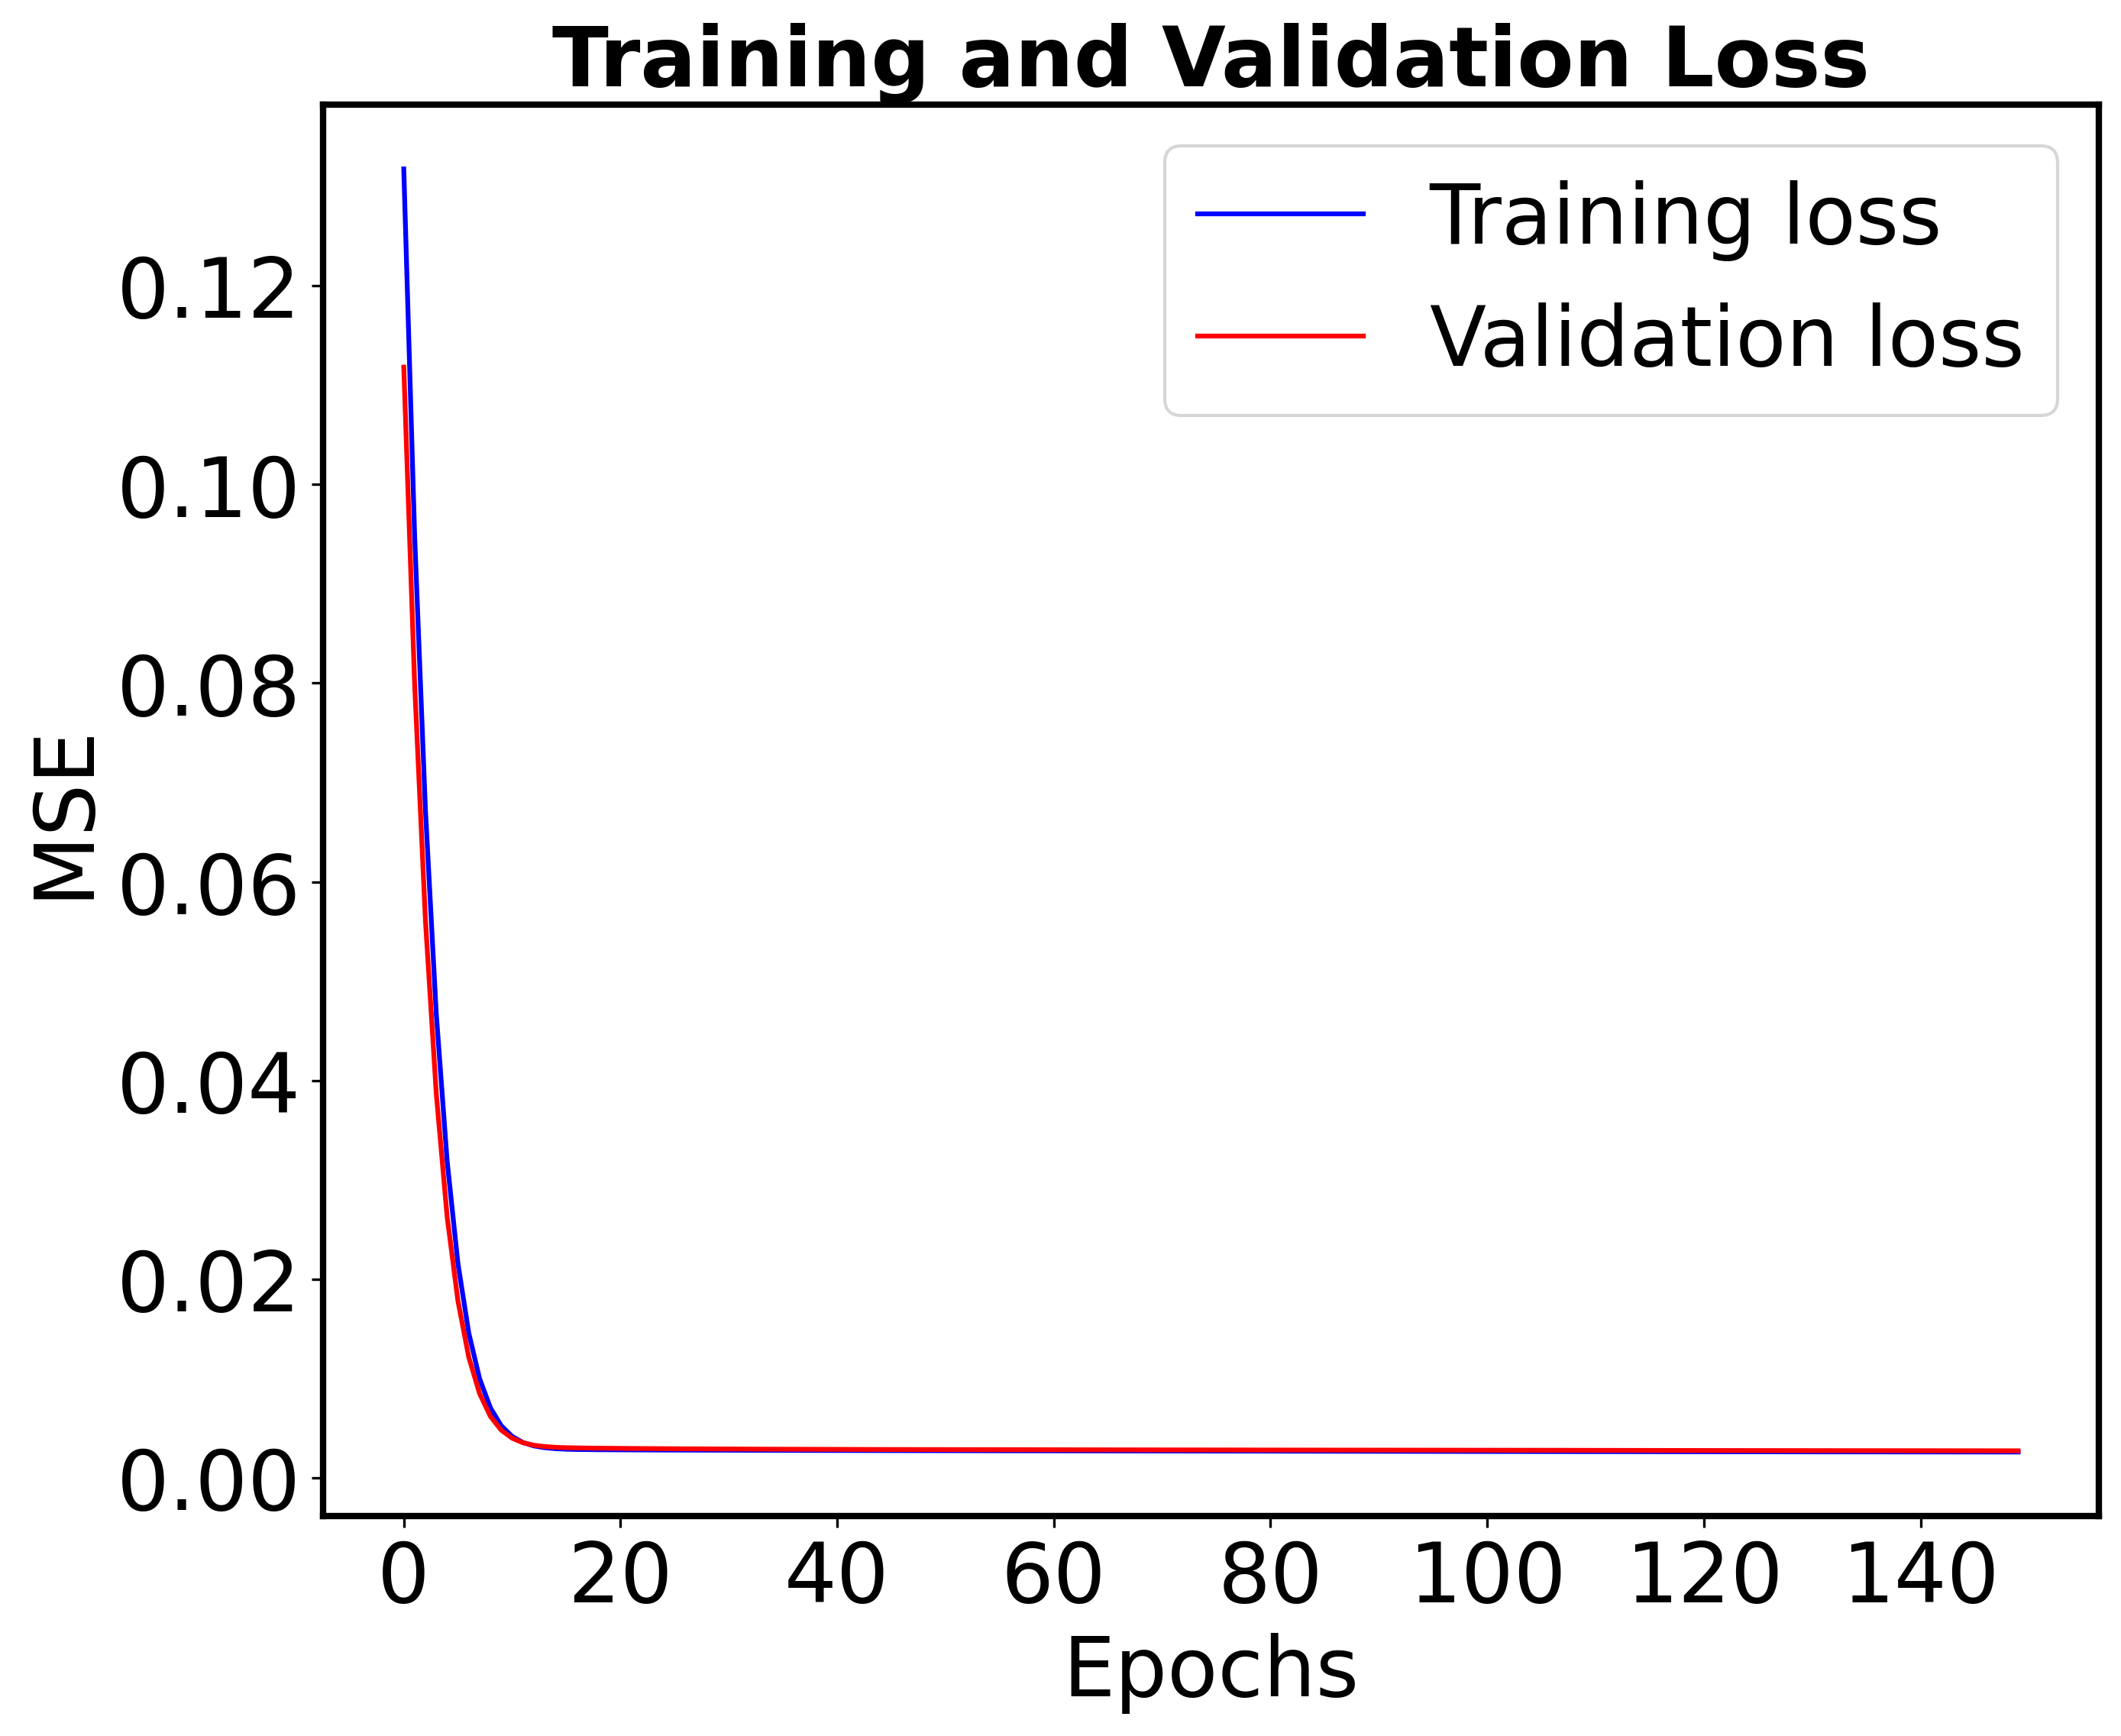
\includegraphics[width=1\linewidth]{Model3_Serie2.png}
	\caption{Model 3 - Serie 2}
	\end{subfigure}
	\caption{The evolution of the MSE on the training and validation sets.}
	\label{fig:training_validation}
\end{figure}



\section{Performance on the test set}
In this section the results on the test set are discussed for the models that were selected in section \ref{s:Model selection}. 
Also, the two best baseline models ``mean forecast'' and ``MAPE forecast'', that were explained in Section \ref{s:Baseline models}, are included in the comparison. An advantage that the baseline models have in comparison to the LSTM neural networks is that they use the previous data till the day to forecast to make predictions while the LSTM neural networks only trains on data till November. (Seeding not taken into account) This is because it needs data for the validation set to tune parameters and implement early stopping. \\

The baseline models and the LSTM neural networks both belong to a different group of models, respectively to the lazy models and eager models. A lazy model only looks at the data when the query is known i.e. what day to forecast. For example a ``mean forecast'' looks after it knows which day to forecast to the same weekdays and takes the average. In comparison an eager model already makes generalizations on a training set before it knows which day it has to predict. This applies to the LSTM models.\\

Model 1 and Model 2 make use of a lag value of $ 48 $ or $ 96 $ and no seeding. When the day after a missing day(s) is predicted the inputs used during prediction could originate entirely from an estimated reference signal for the missing day(s). If this is the case, it is expected that the error on the desired day will be larger. The estimation of the reference signal is done by substituting the missing values as described in Section \ref{s:Preprocessing_cha4}. For both Serie 1 and Serie 2 there are $ 8 $ missing days in the test set.

\begin{figure}[h]
	\centering
	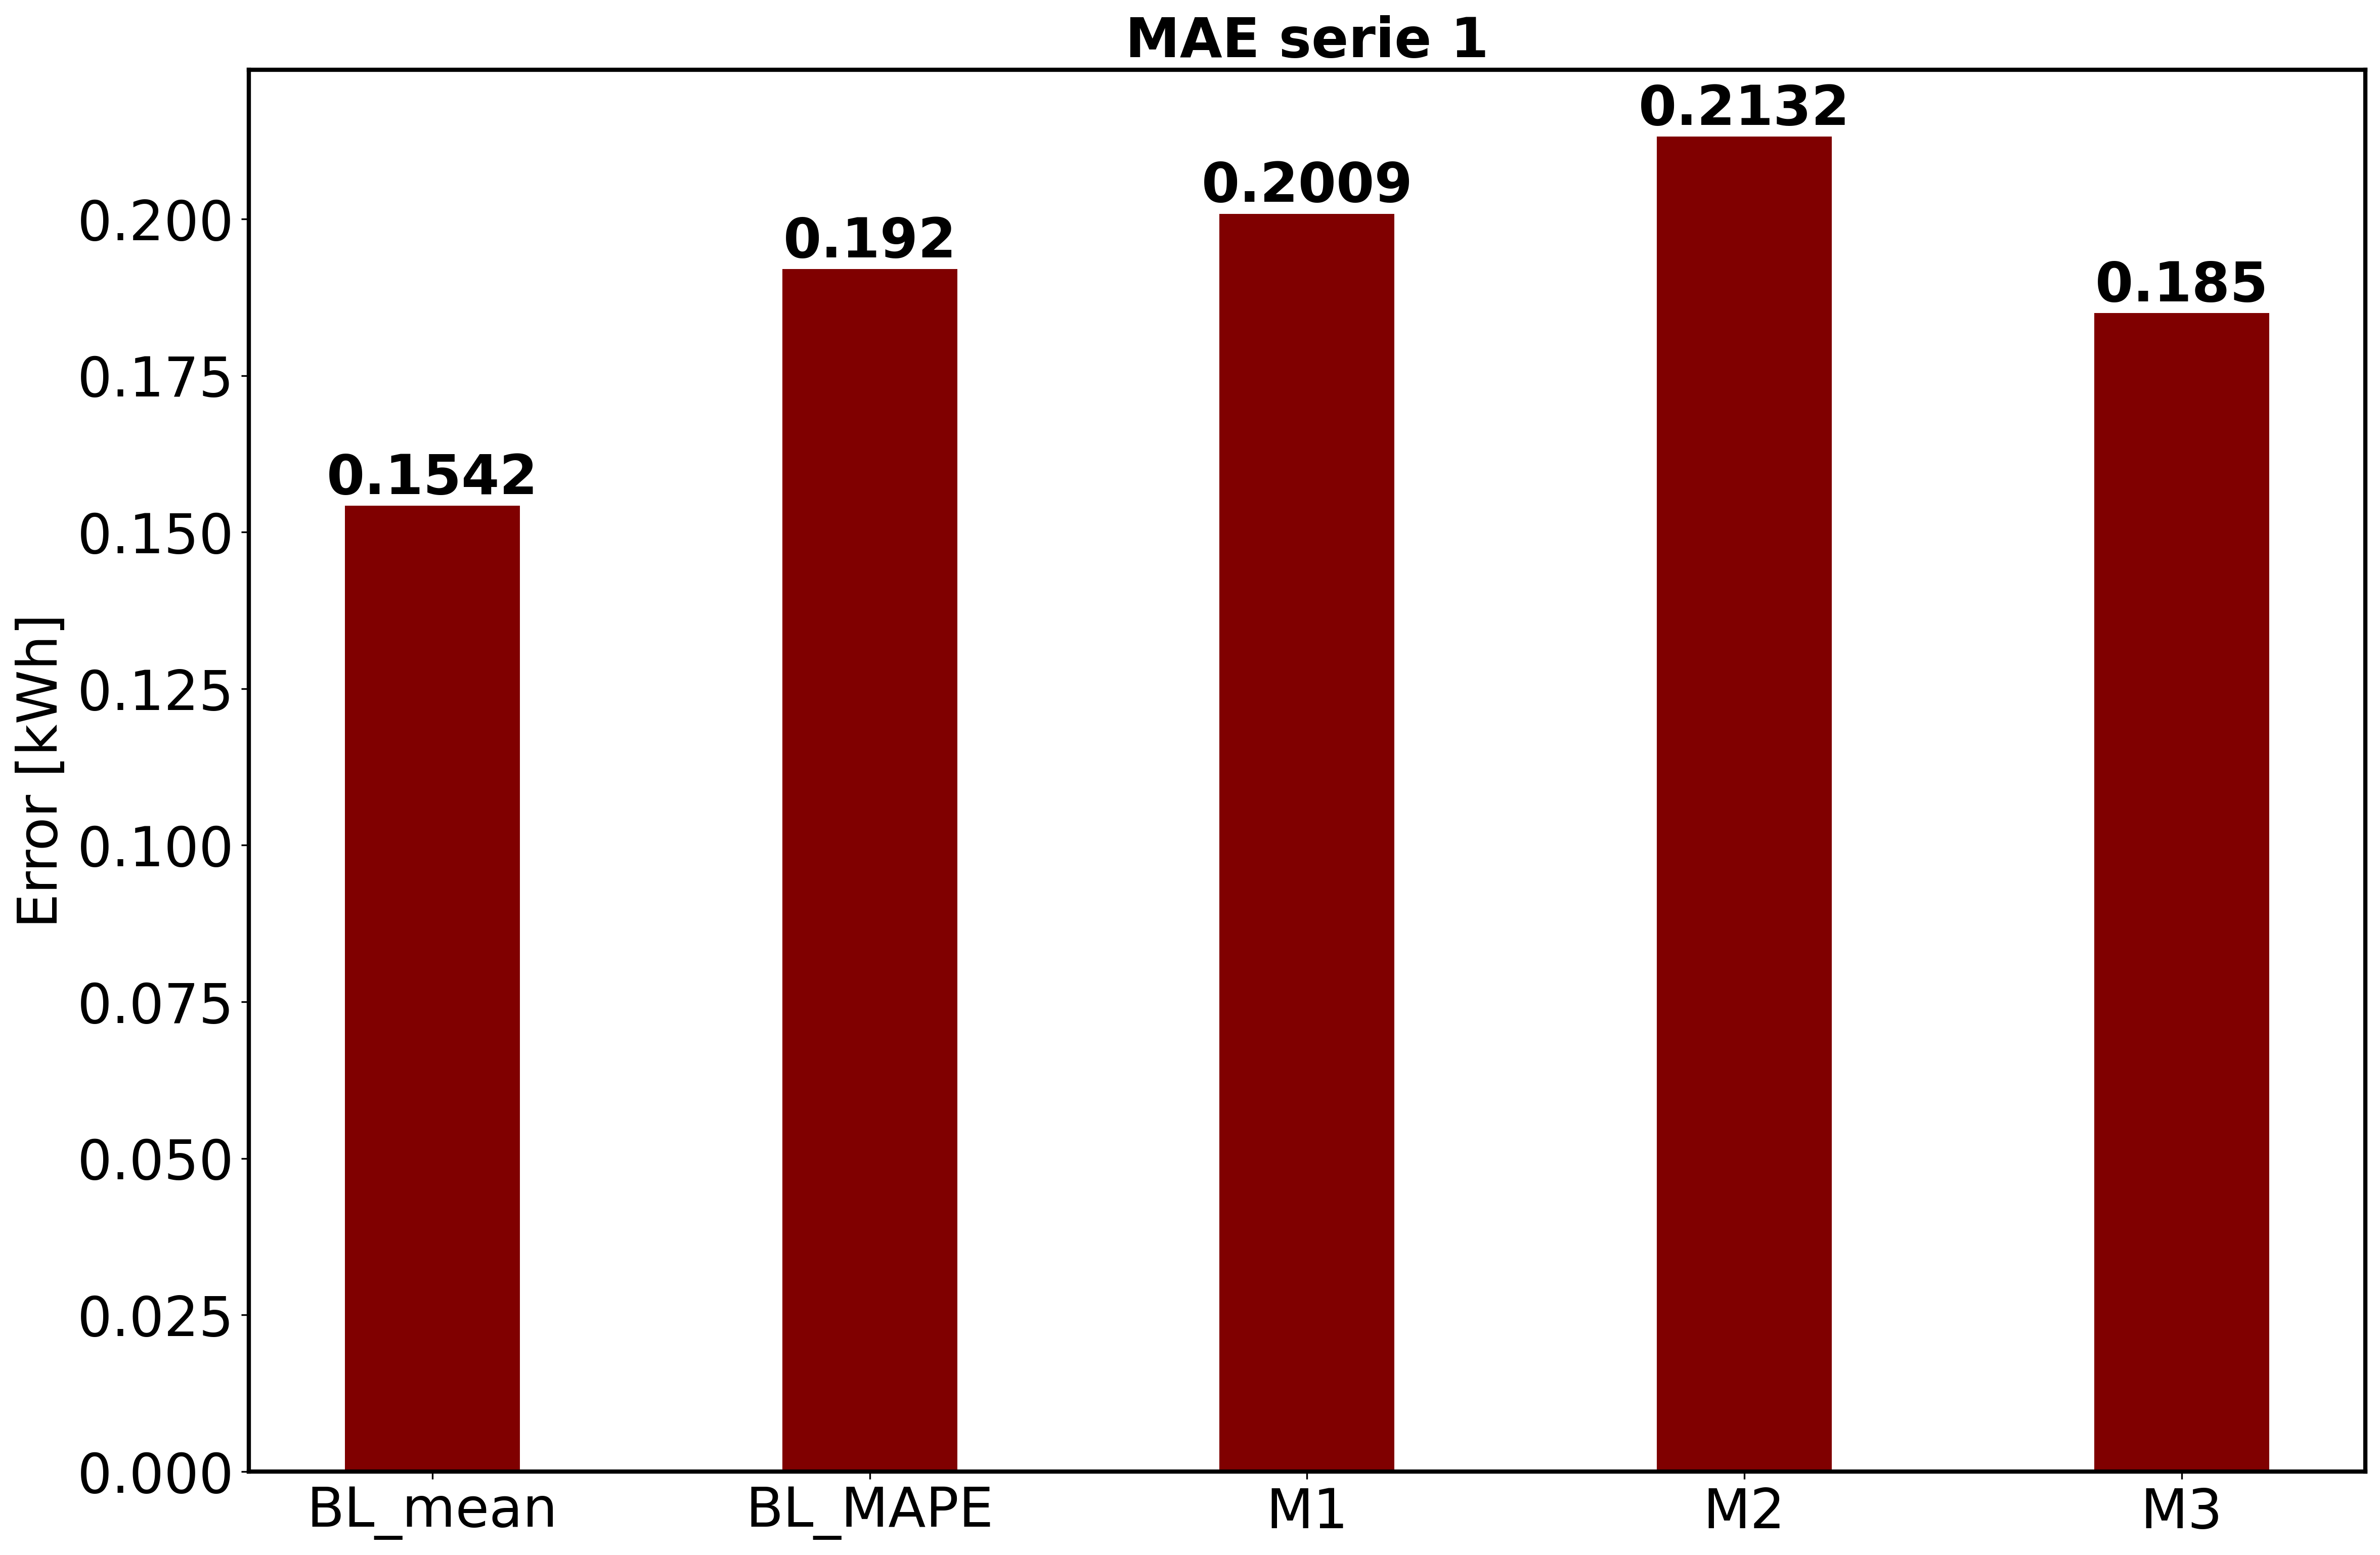
\includegraphics[width=0.8\linewidth]{MAE_1.png}
	\caption{The MAE performance on all the days of the test set for Serie 1.}
	\label{fig:MAE_serie1}
\end{figure}

\begin{figure}[h]
	\centering
	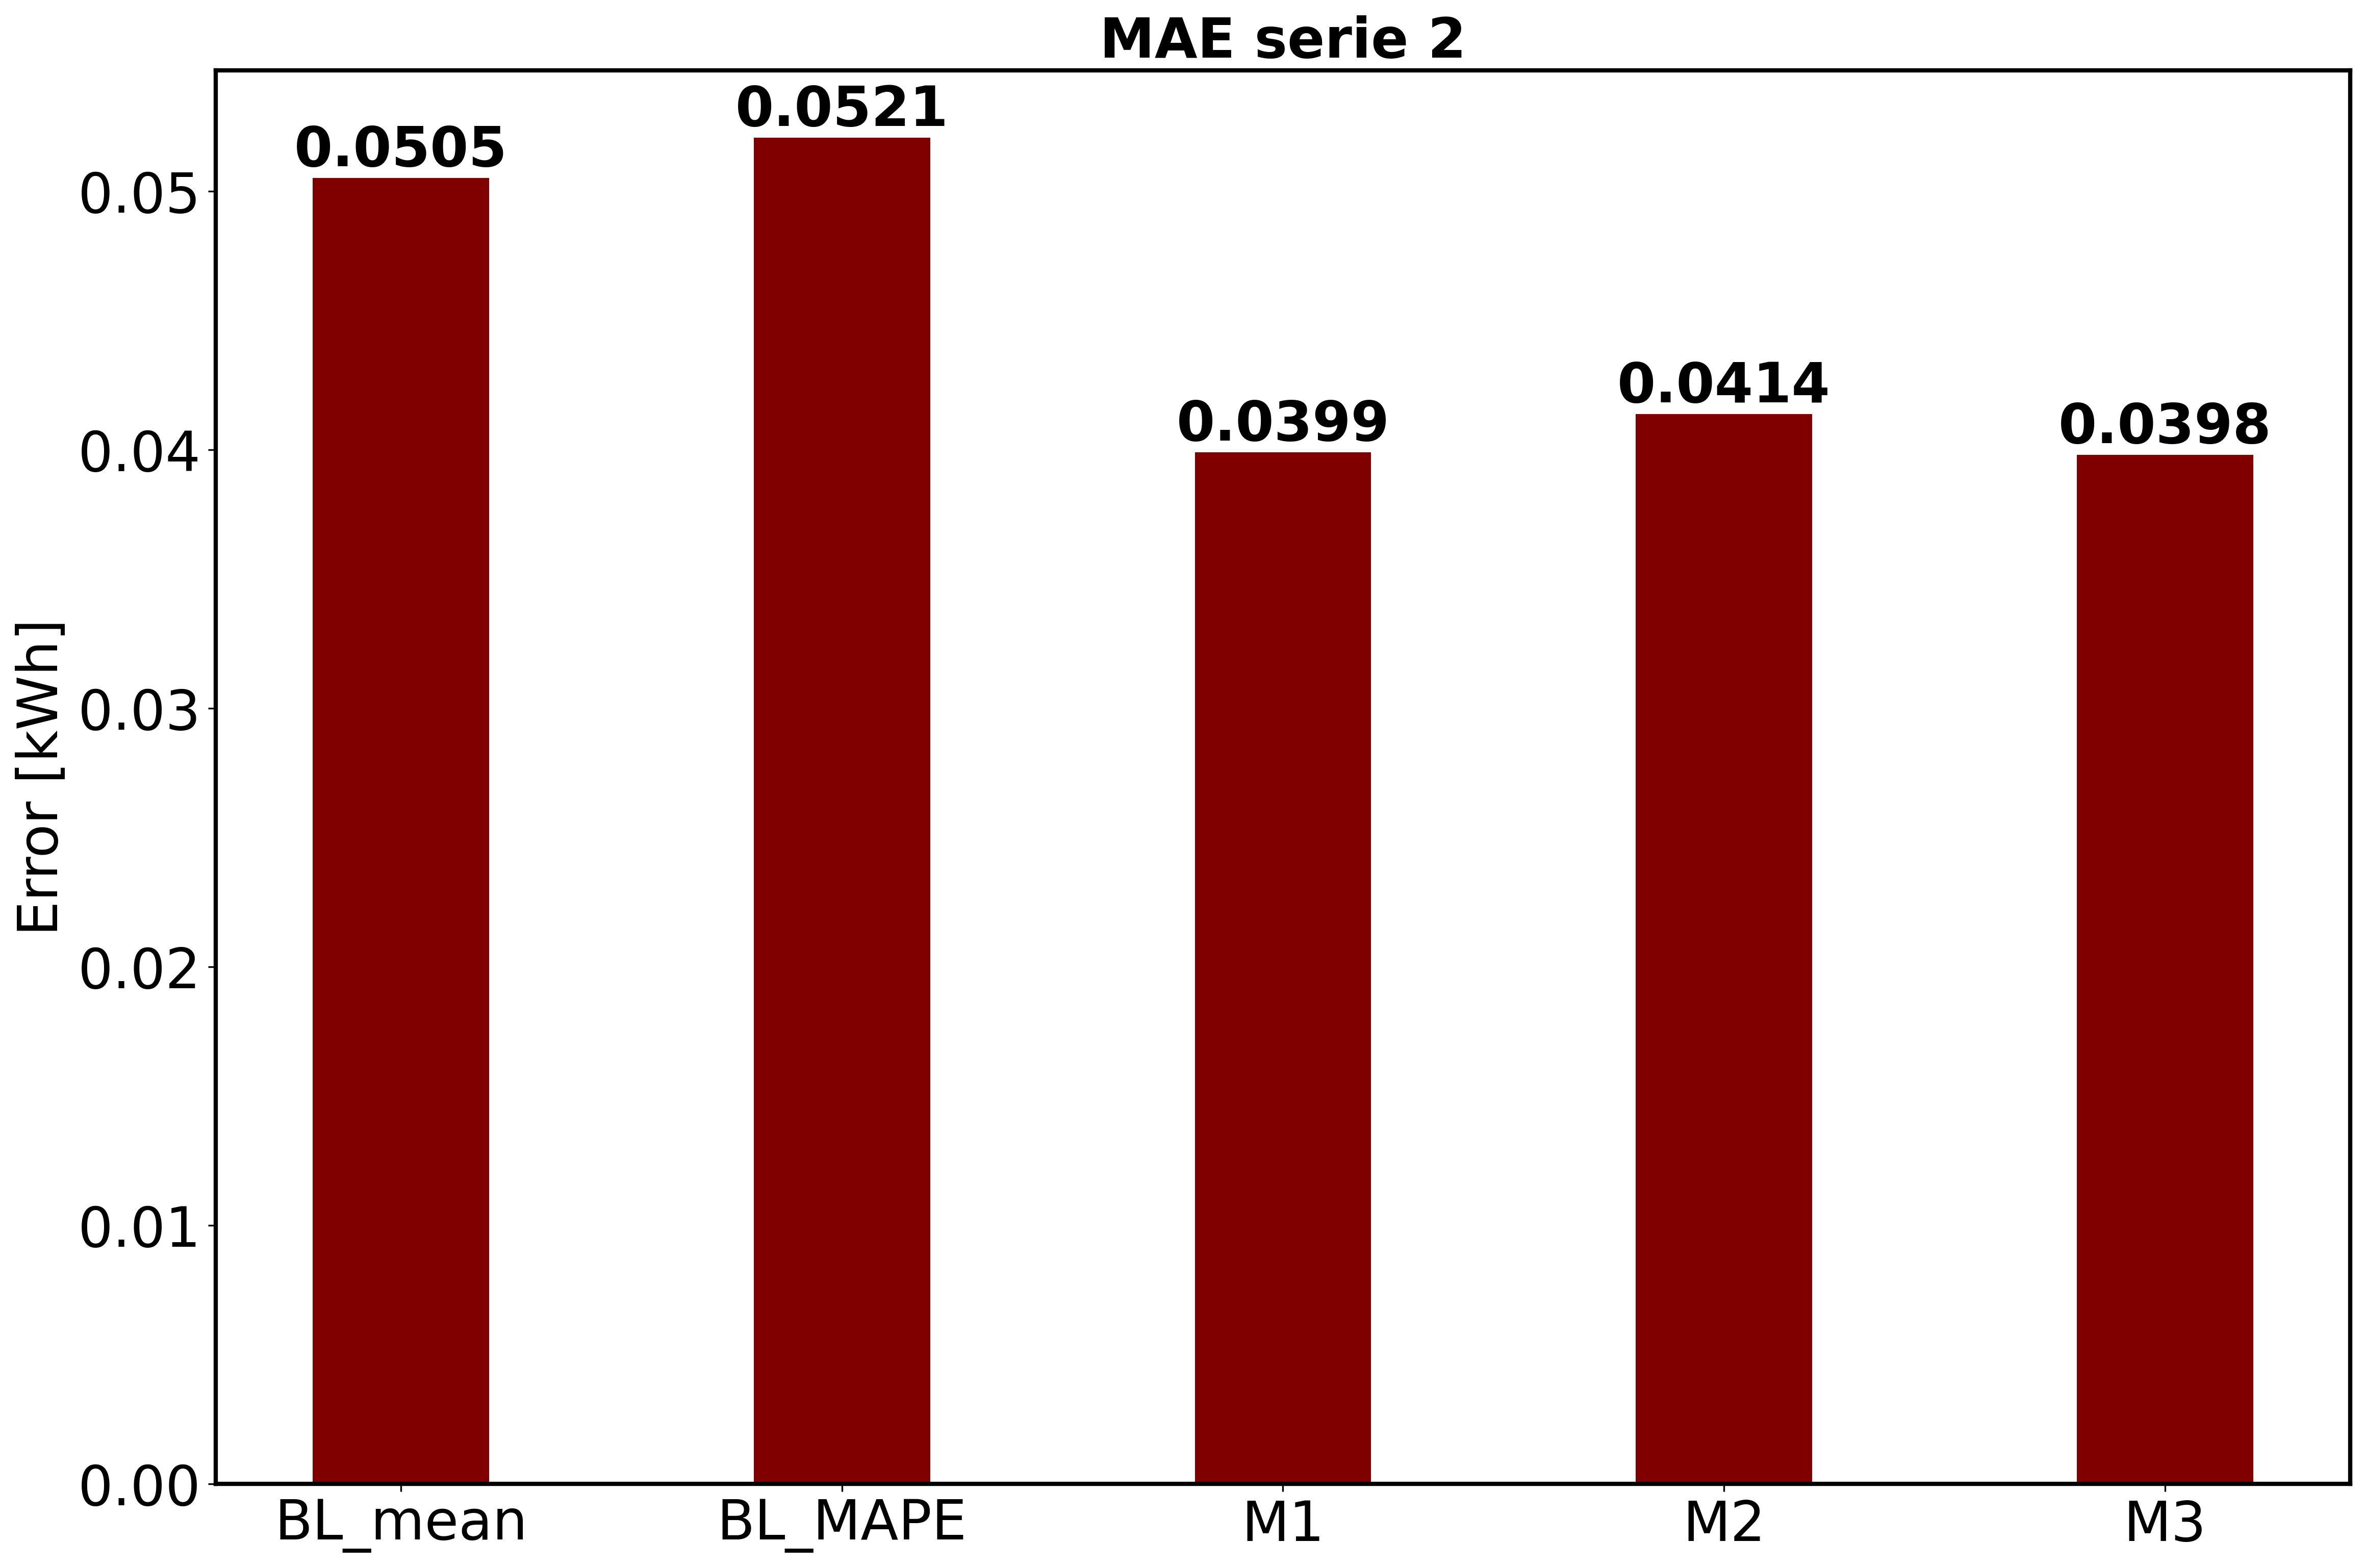
\includegraphics[width=0.8\linewidth]{MAE_2.png}
	\caption{The MAE performance on all the days of the test set for Serie 2.}
	\label{fig:MAE_serie2}
\end{figure}	

\begin{figure}[h]
	\centering
	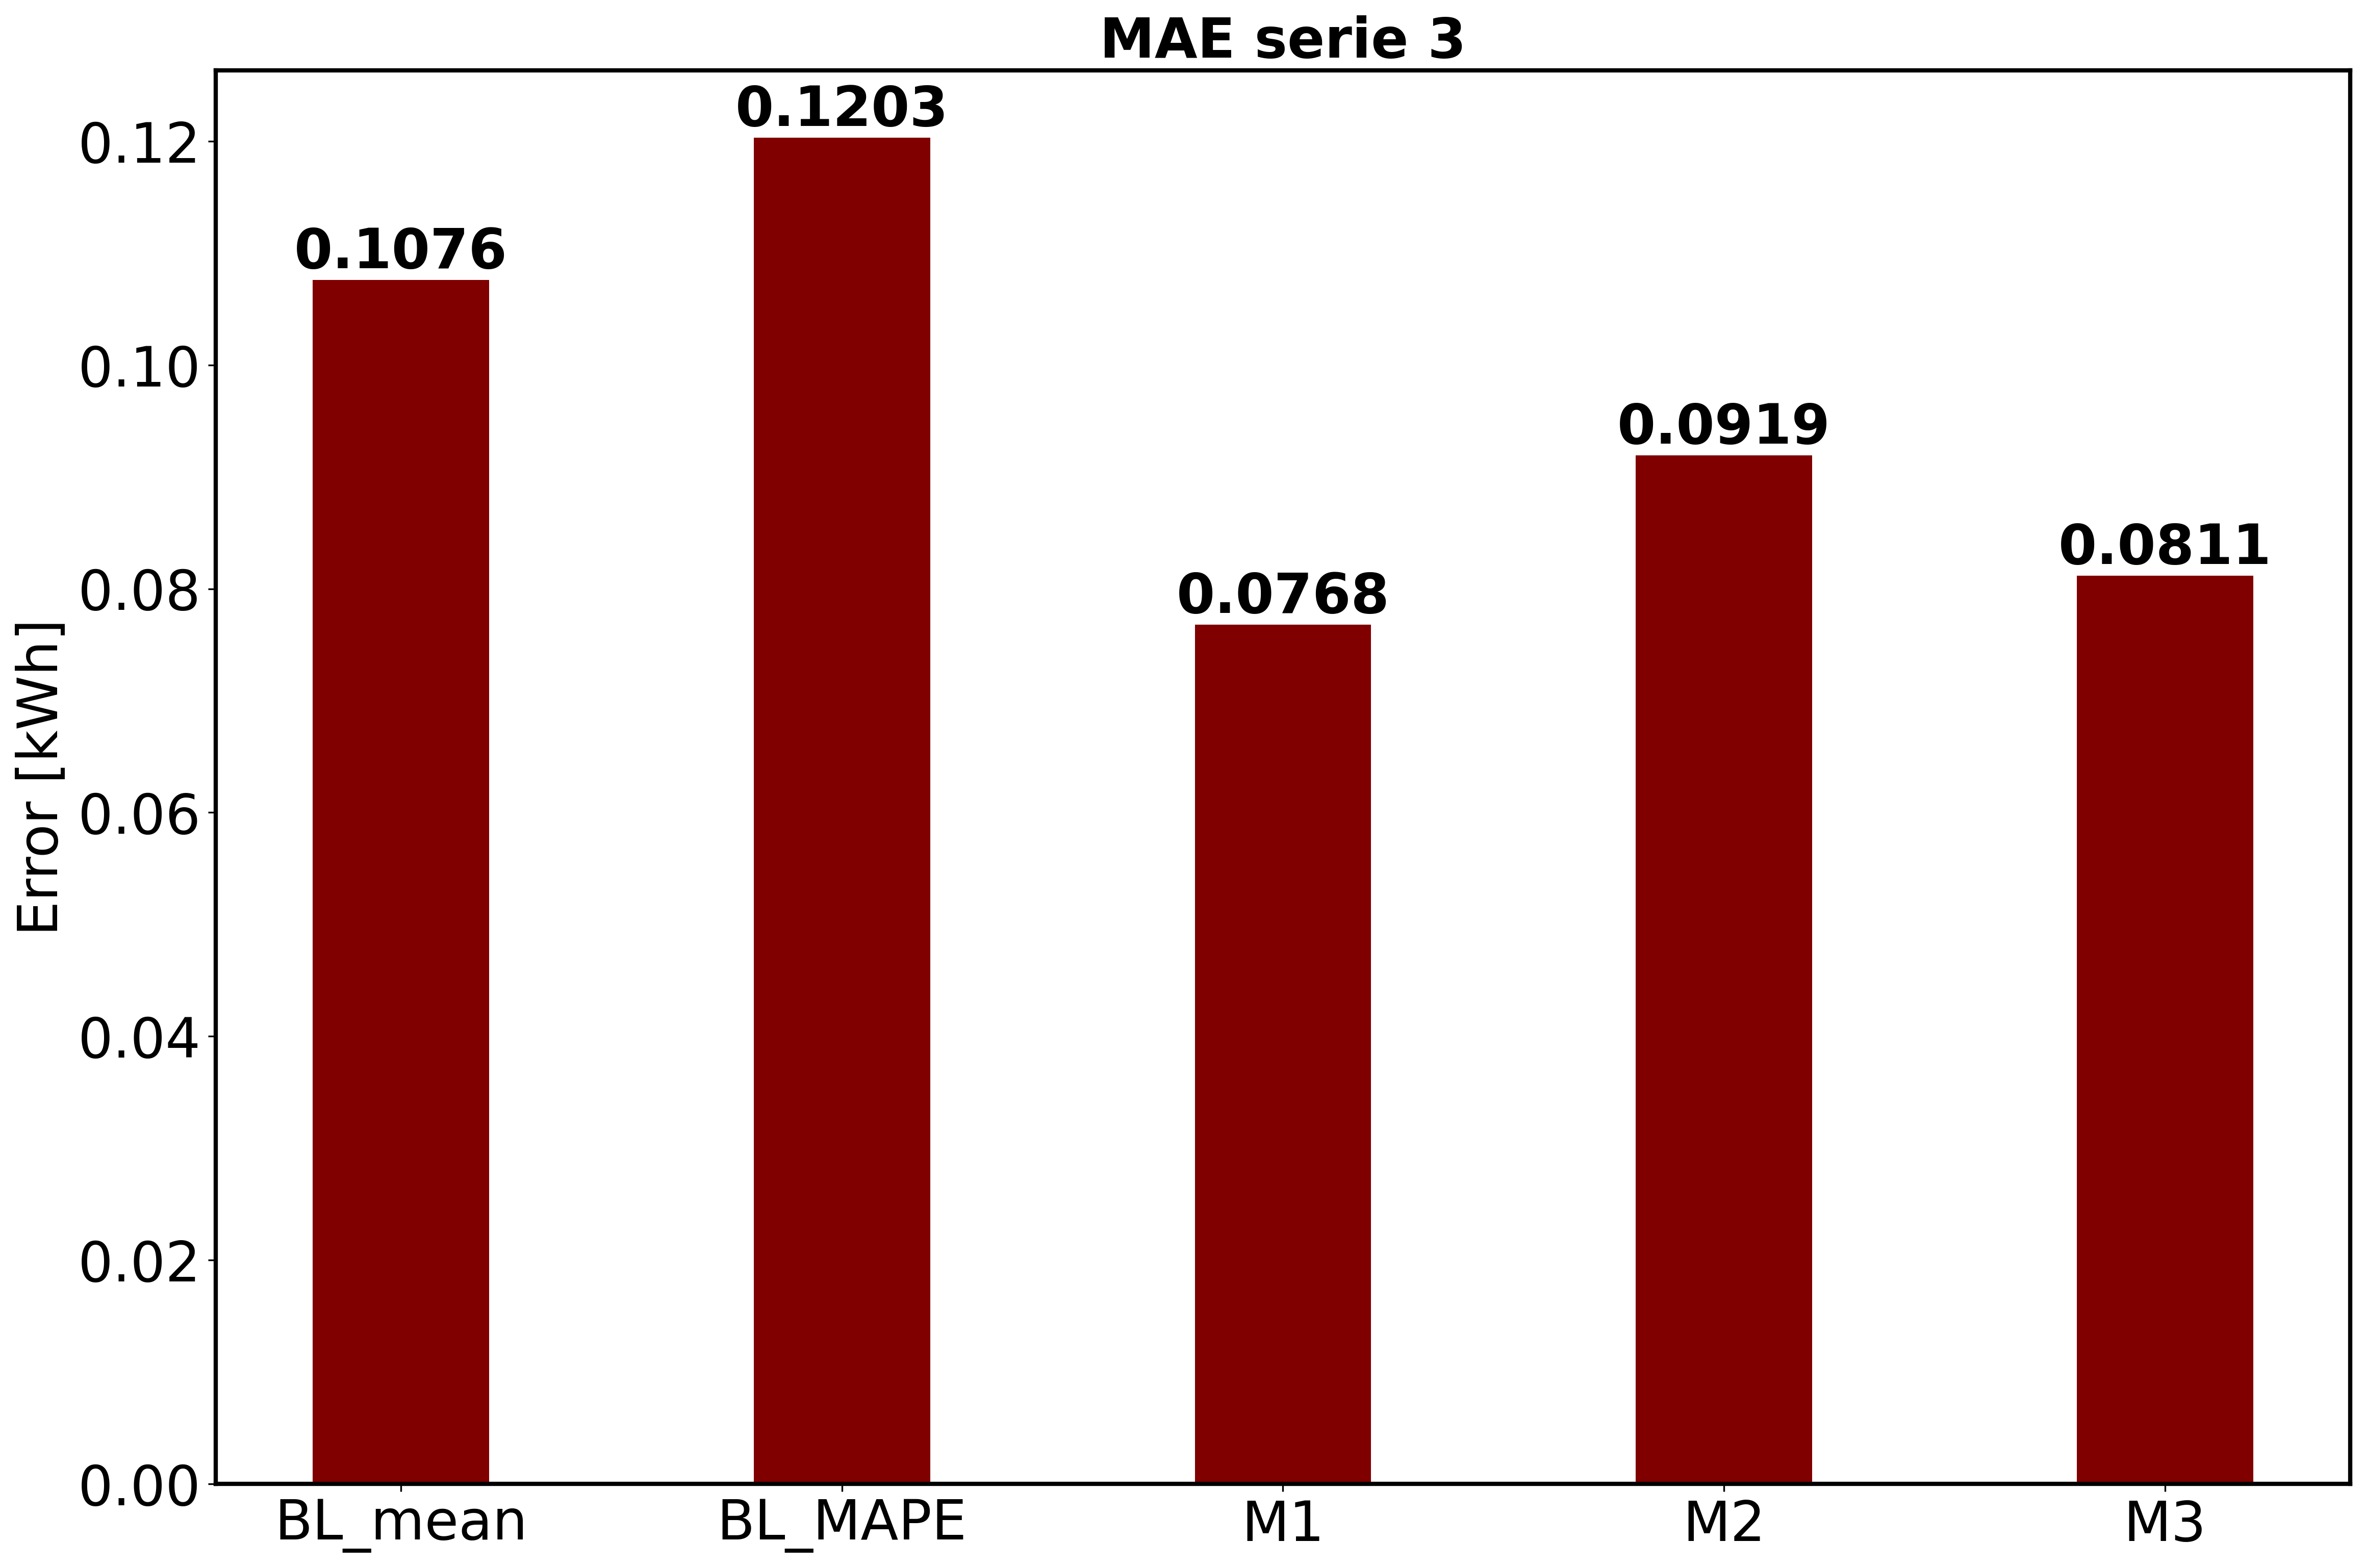
\includegraphics[width=0.8\linewidth]{MAE_3.png}
	\caption{The MAE performance on all the days of the test set for Serie 3.}
	\label{fig:MAE_serie3}
\end{figure}	

Figures \ref{fig:MAE_serie1}, \ref{fig:MAE_serie2} and \ref{fig:MAE_serie3} give a comparison of the three LSTM models and the two baseline models. It can be seen that there is a reduction of the MAE for Series 2 and 3 for all the LSTM models and for Serie 1, Model 3 attains a smaller error than the ``MAPE forecast'' model. Also, it can be noticed that Model 2 for all the three series behaves slightly worse than the other two LSTM models. It is clear that the performance of the models is serie dependent.\\

To get more insight in how the MAE error is distributed over the test set, it is calculated for each individual day and displayed in Figures \ref{fig:MAE_line_serie1}, \ref{fig:MAE_line_serie2} and \ref{fig:MAE_line_serie3} in Appendix \ref{app:Extensions on the evaluation results}. Figures \ref{fig:MAE_line_serie2} and \ref{fig:MAE_line_serie3} are discontinuous due to the missing days that are present in the reference signal in the month December. When the reference values of a day are not known, the day is removed from the test set to remove an additional estimation error of the reference signal during the calculation of the MAE. This is also the case for the calculation of the MAE in Figures \ref{fig:MAE_serie1}, \ref{fig:MAE_serie2} and \ref{fig:MAE_serie3}. \\

Next, it is noted that the MAPE for the LSTM models is much higher than for the baseline models as is shown in Table \ref{tab:summary_MAPE_error}. As displayed in Figure \ref{fig:individual_forecasts} this is due to an overestimation of the reference signal when the values are small.\\


\begin{table}[h]
	\centering
	\begin{tabular}{@{}l|ccccc@{}} \toprule
		&\textbf{Mean forecast} & \textbf{MAPE forecast} & \textbf{Model $ 1 $} & \textbf{Model $ 2 $} & \textbf{Model $ 3 $}\\\midrule
		\textbf{Serie 1} & $0.46 $&$ 0.41$  & $3.07 $ & $3.37 $  & $3.27 $\\
		\textbf{Serie 2} & $1.82 $&$ 0.83 $  & $3.67$ & $3.64 $  & $3.65 $\\
		\textbf{Serie 3} & $0.80 $&$ 0.48 $  & $3.30$ & $3.44 $ & $3.21 $\\\bottomrule
	\end{tabular}
	\caption{The MAPE for each Model and serie.}
	\label{tab:summary_MAPE_error}
\end{table}

To get better insight in the actual output of the different models, Figure \ref{fig:individual_forecasts} shows the prediction of the different models on a chosen day in the test set.\\
 
 \begin{figure}[ht]
 	\begin{subfigure}{0.32\textwidth}
 		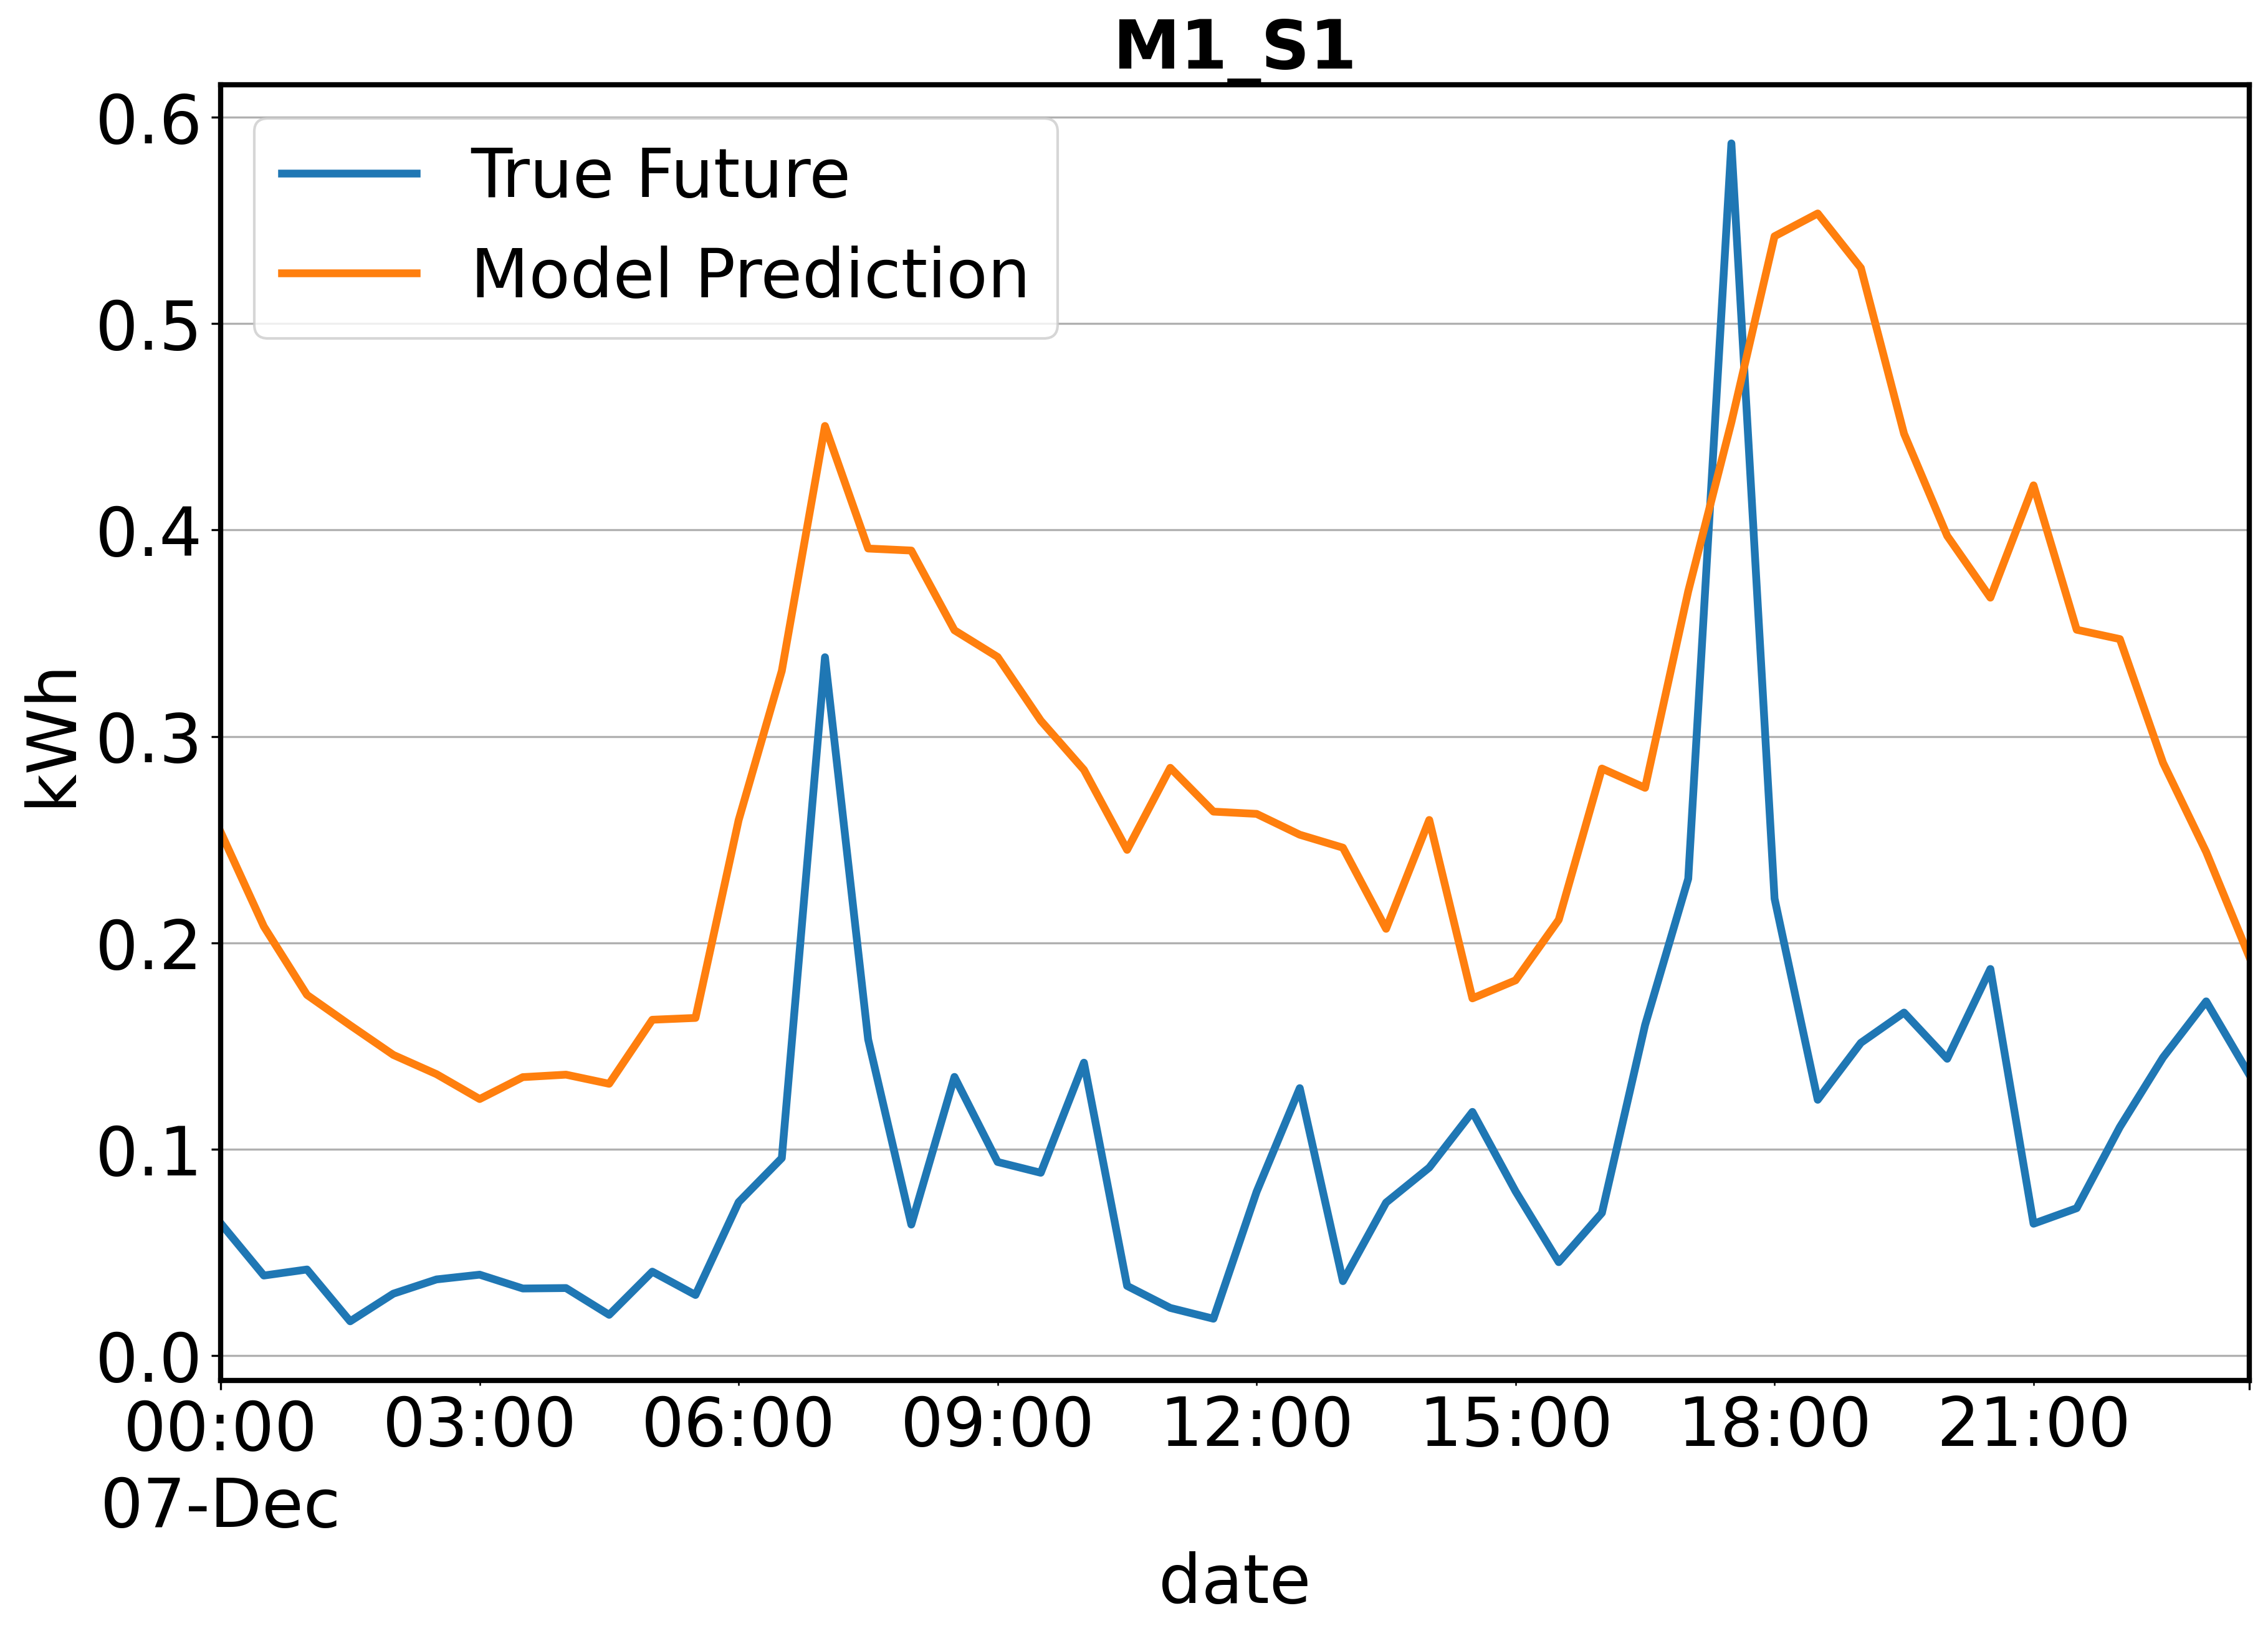
\includegraphics[width=1\linewidth]{IDM1_S1_Day341.png}
 		\caption{Model $ 1 $ - Serie $ 1 $}
 	\end{subfigure}	 	
 	\begin{subfigure}{0.32\textwidth}
 		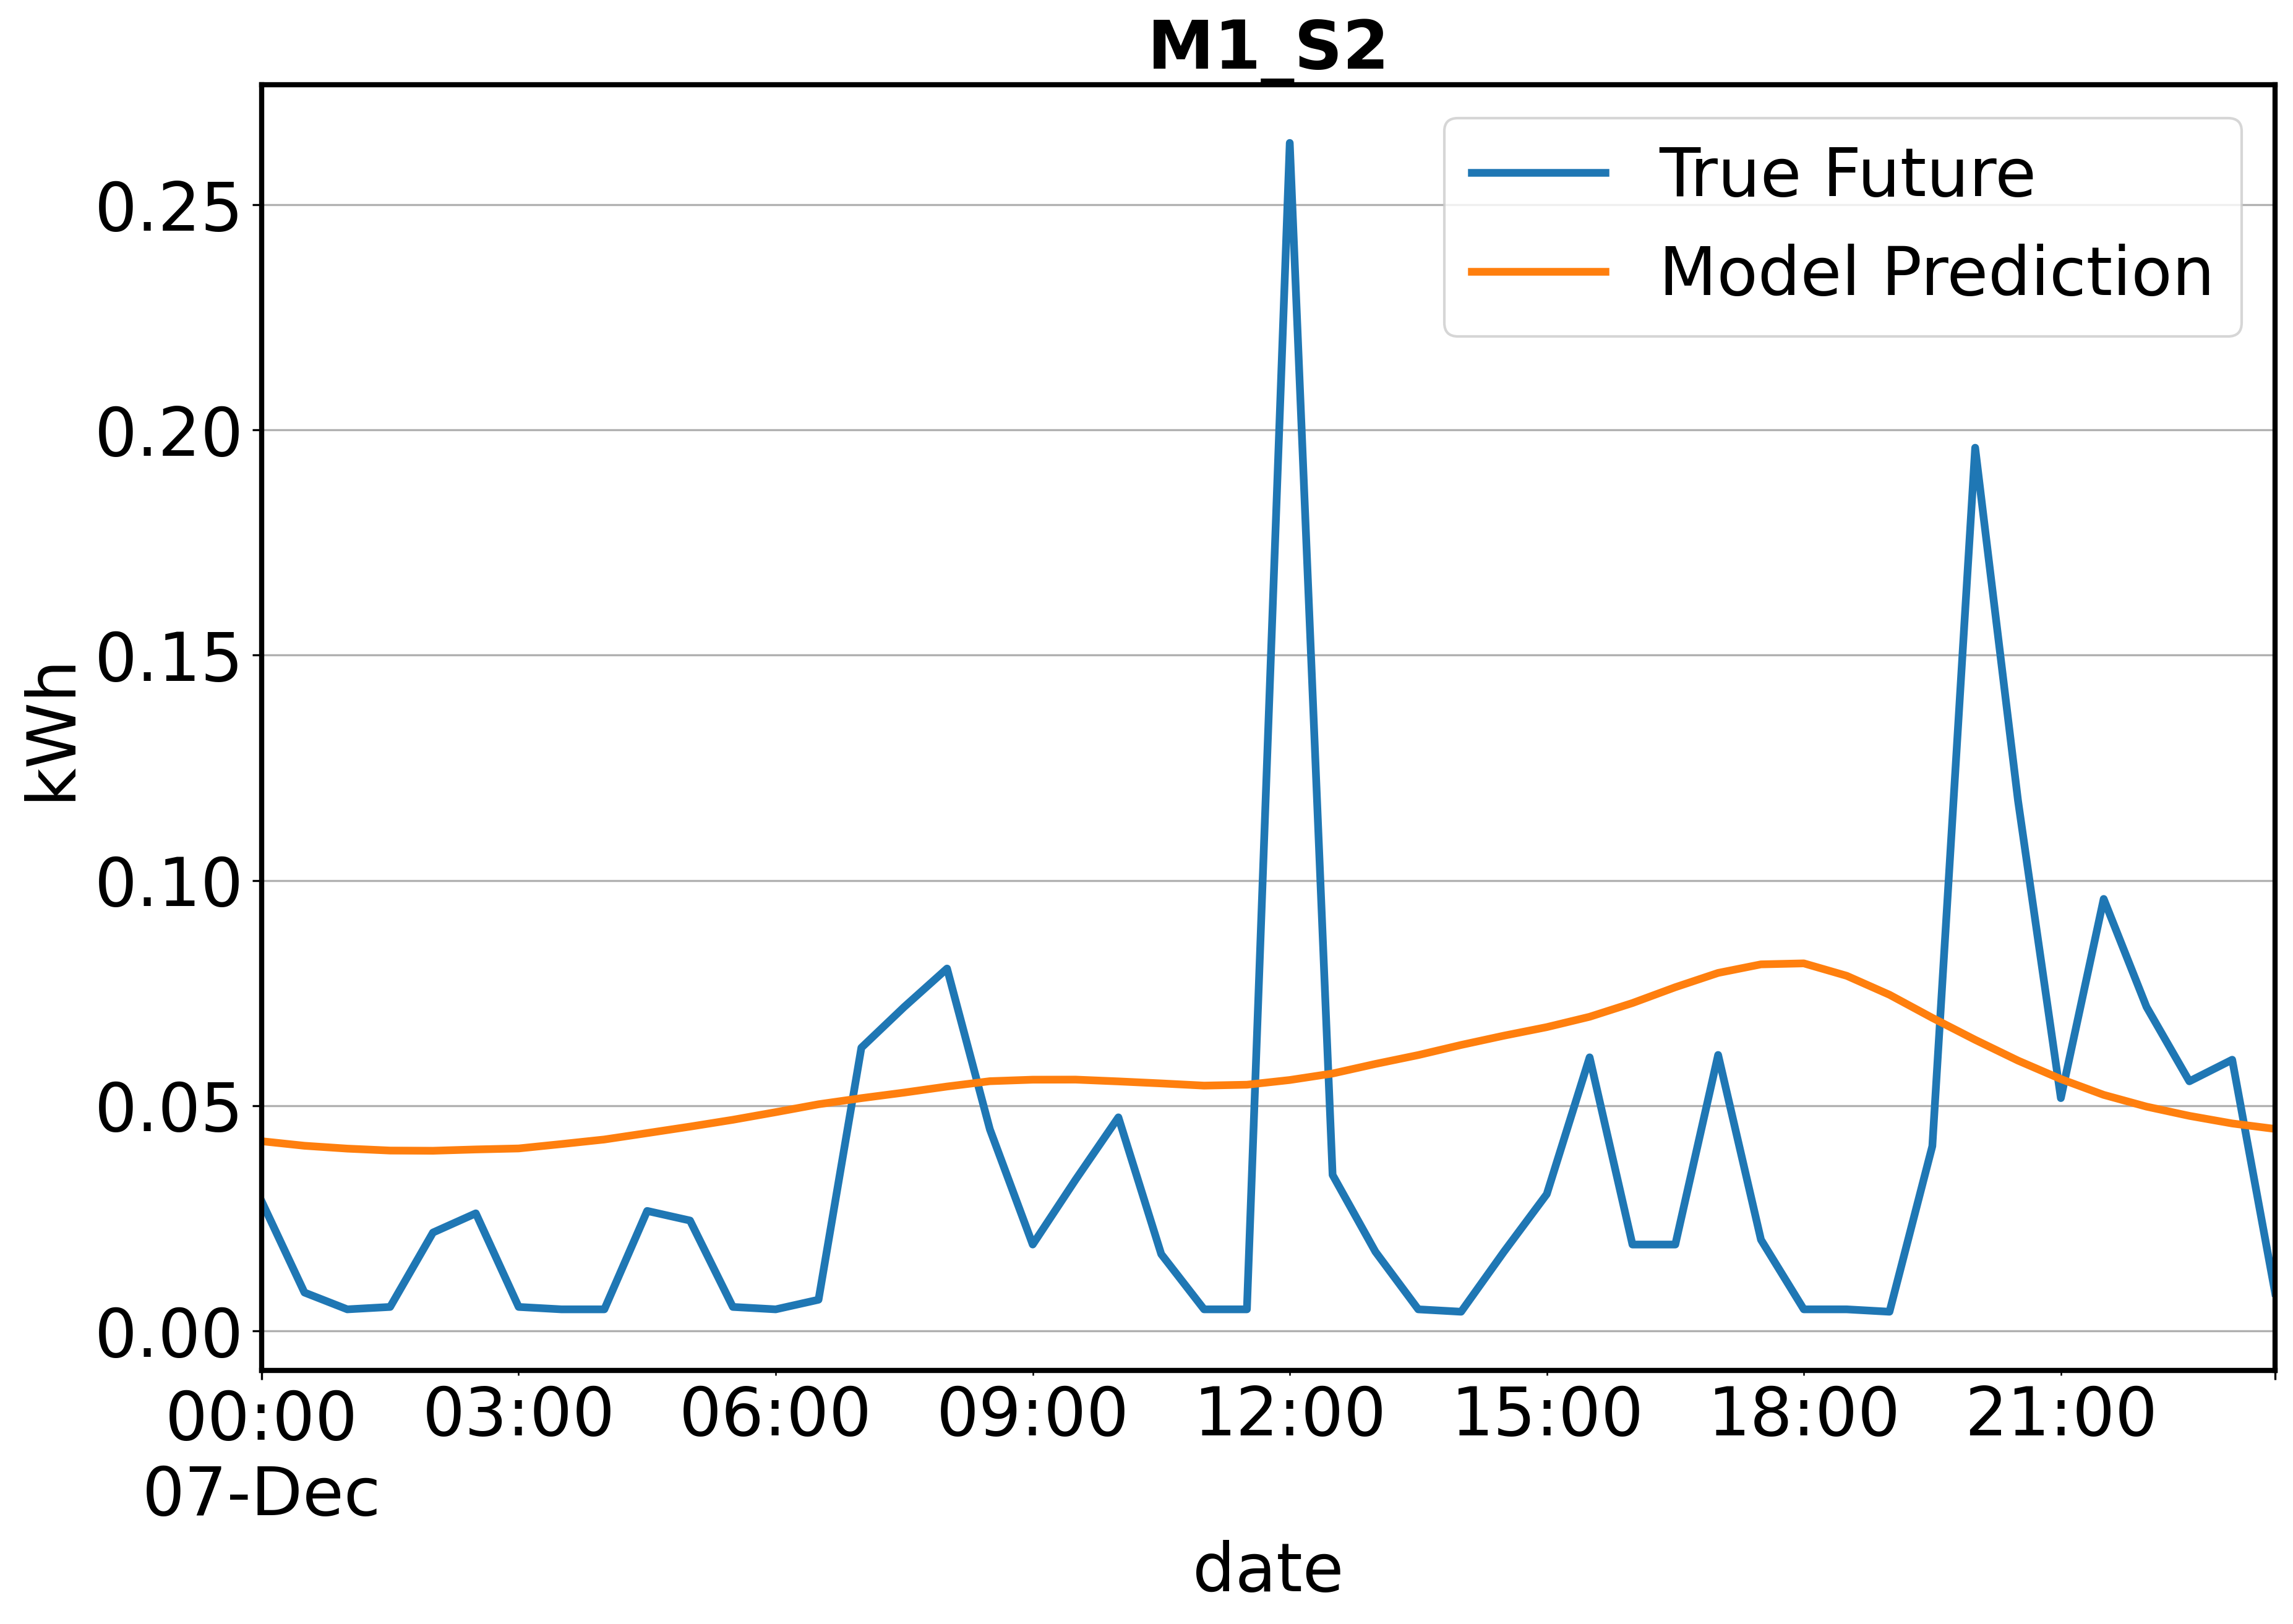
\includegraphics[width=1\linewidth]{IDM1_S2_Day341.png}
 		\caption{Model $ 1 $ - Serie $ 2 $}
 	\end{subfigure}	
 	\begin{subfigure}{0.32\textwidth}
 		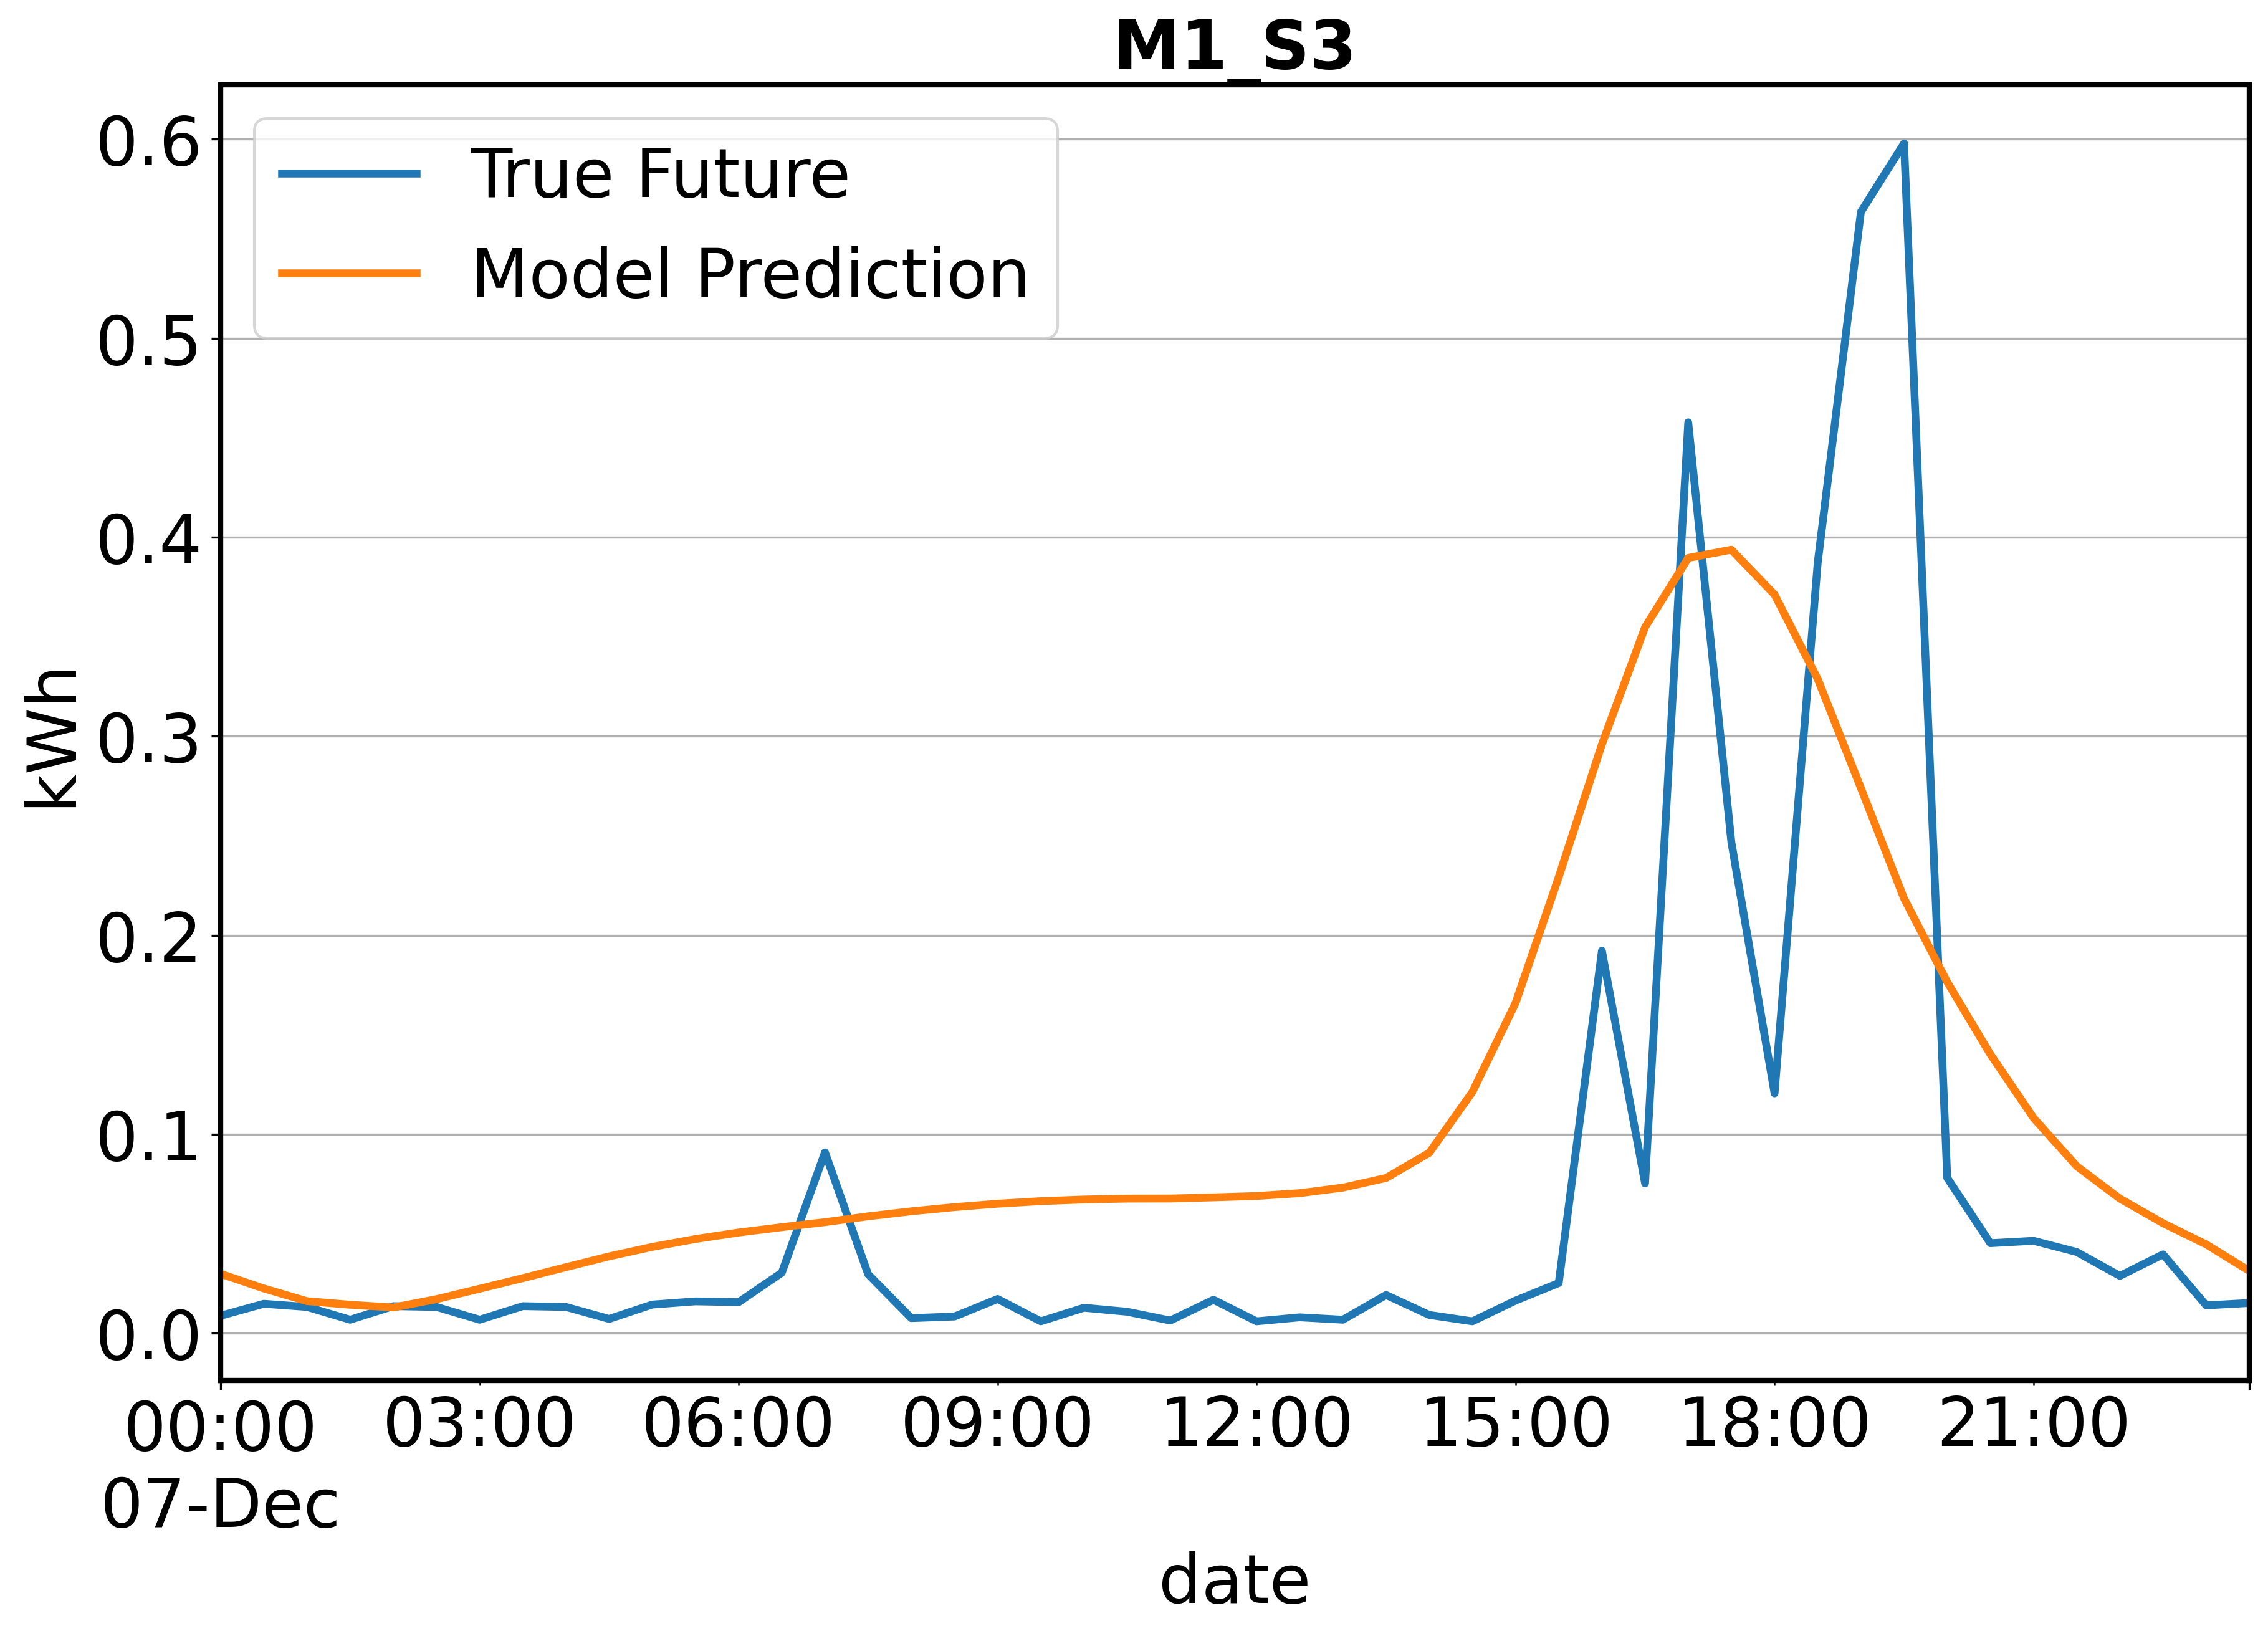
\includegraphics[width=1\linewidth]{IDM1_S3_Day341.png}
 		\caption{Model $ 1 $ - Serie $ 3 $}
 	\end{subfigure}
  	\begin{subfigure}{0.32\textwidth}
 		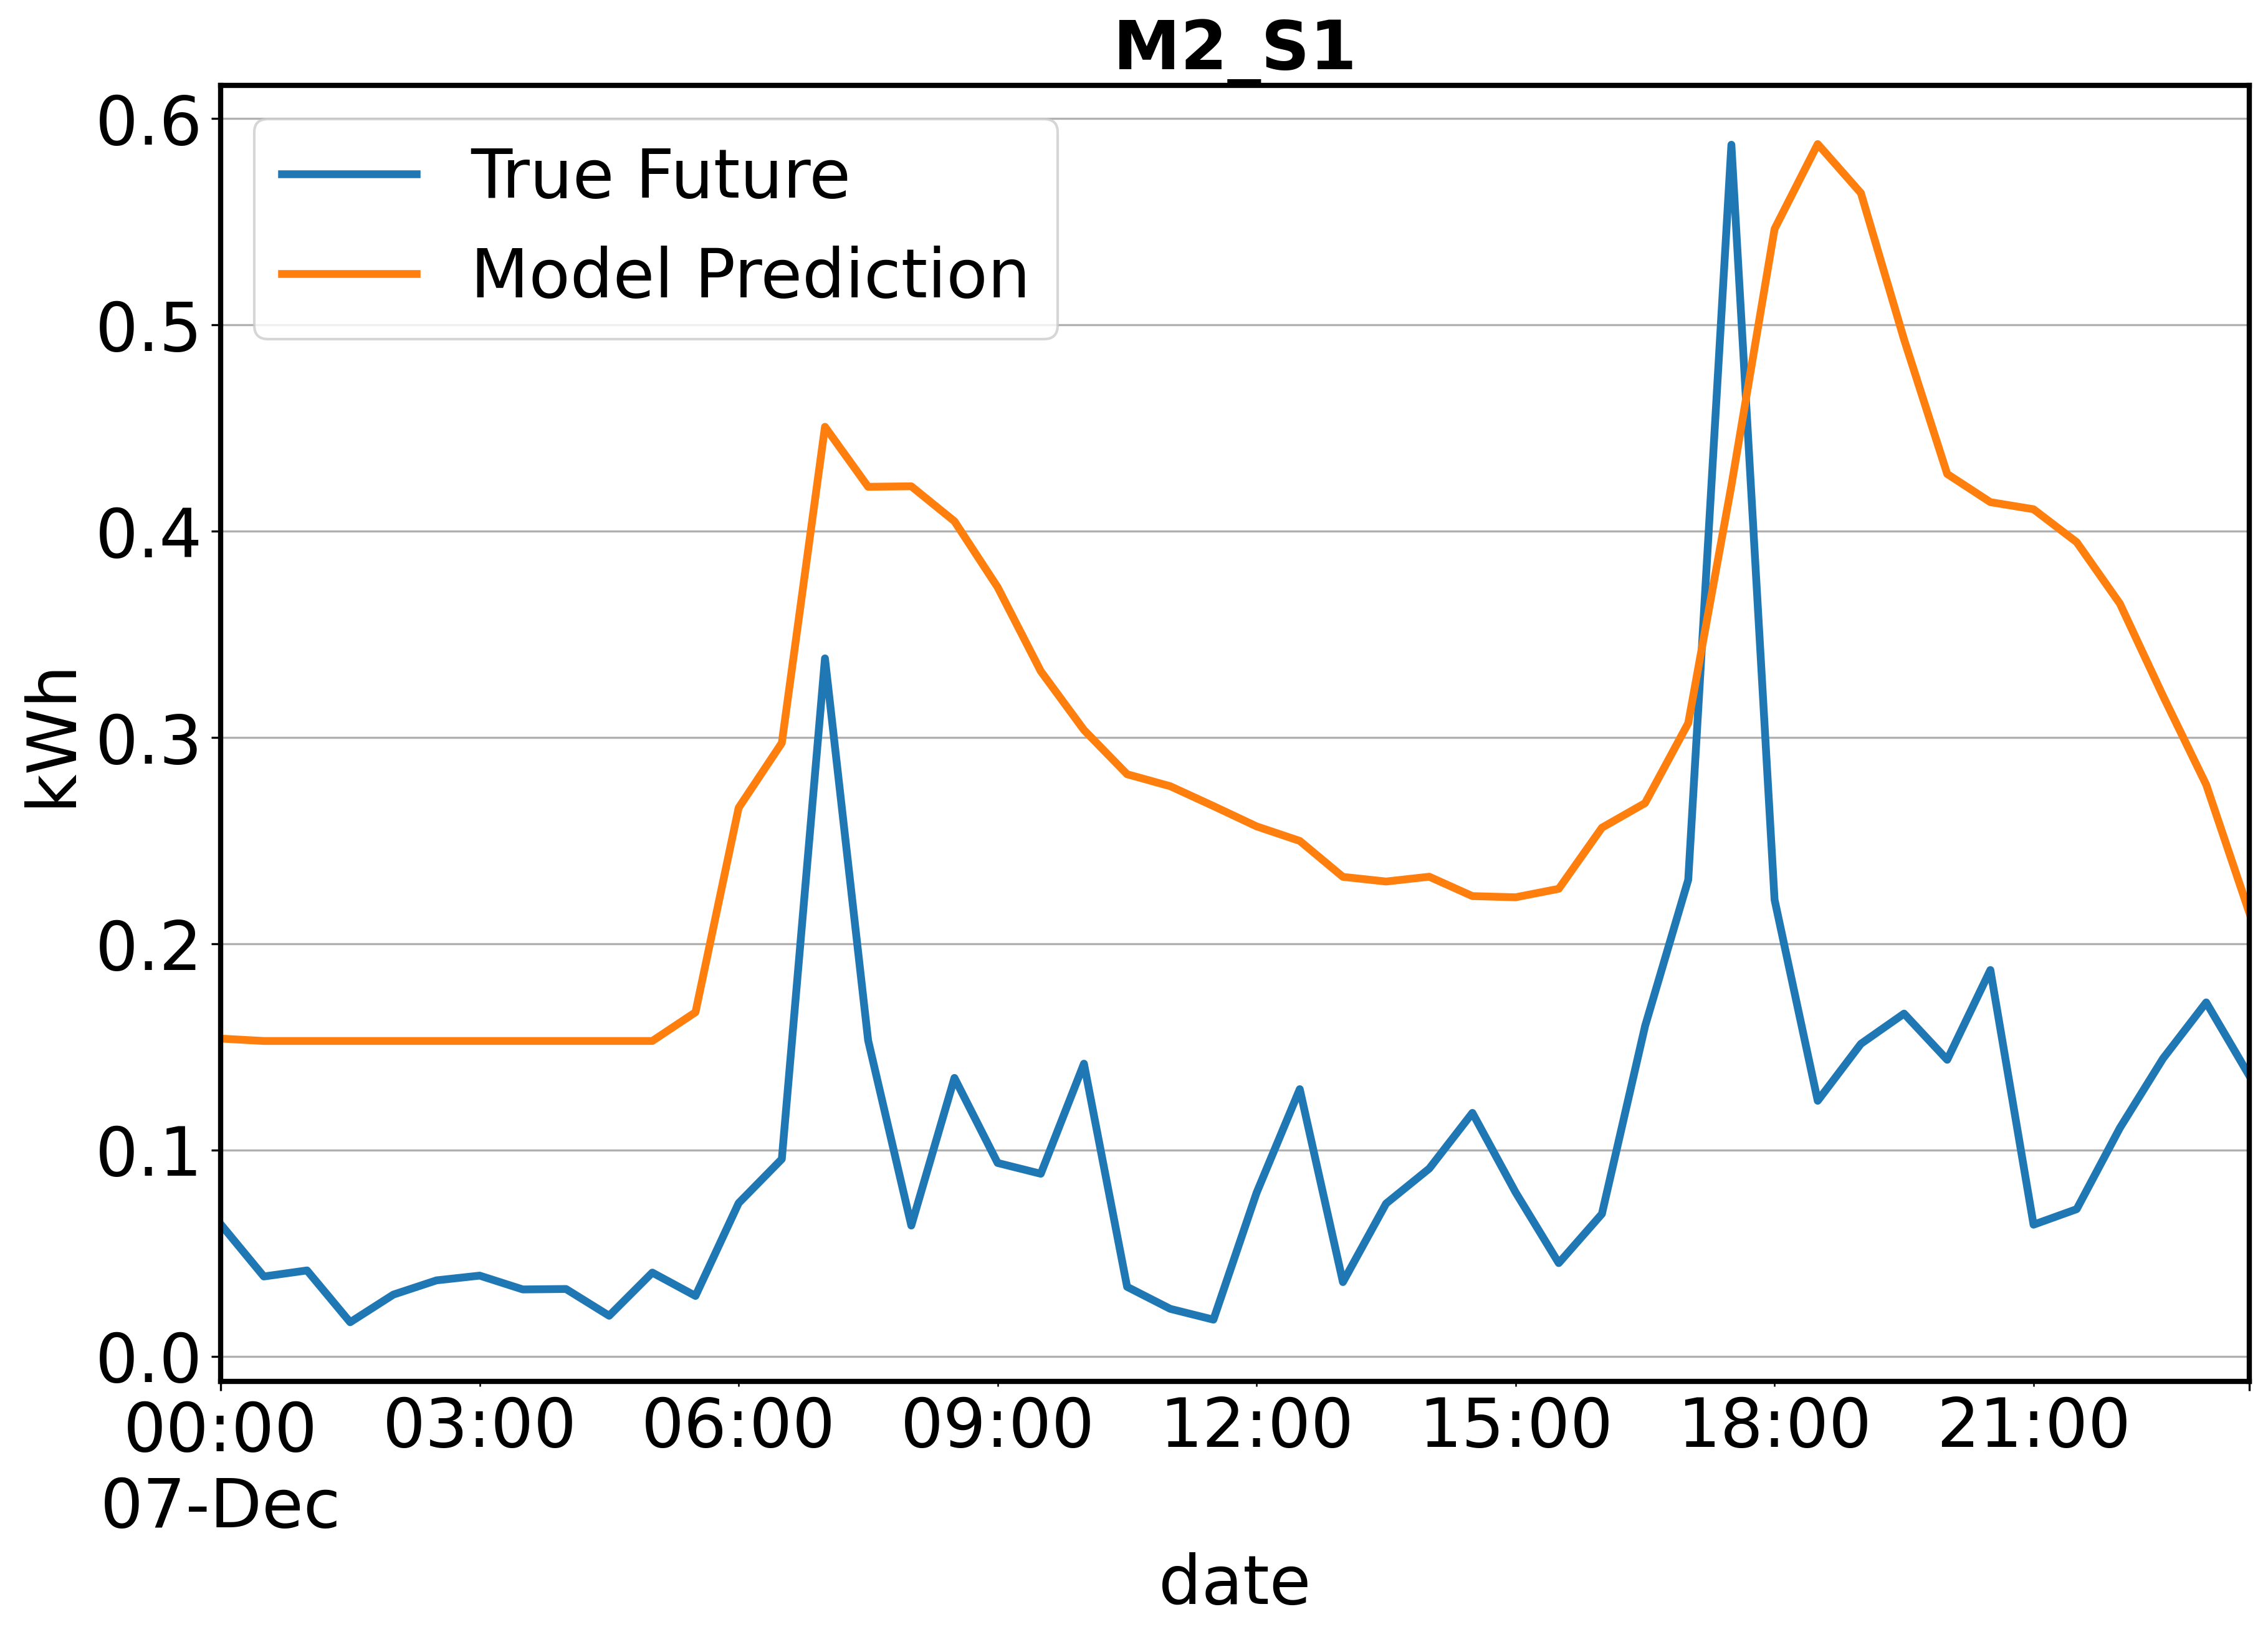
\includegraphics[width=1\linewidth]{IDM2_S1_Day341.png}
 		\caption{Model $ 2 $ - Serie $ 1 $}
 	\end{subfigure}	 	
	 \begin{subfigure}{0.32\textwidth}
	 	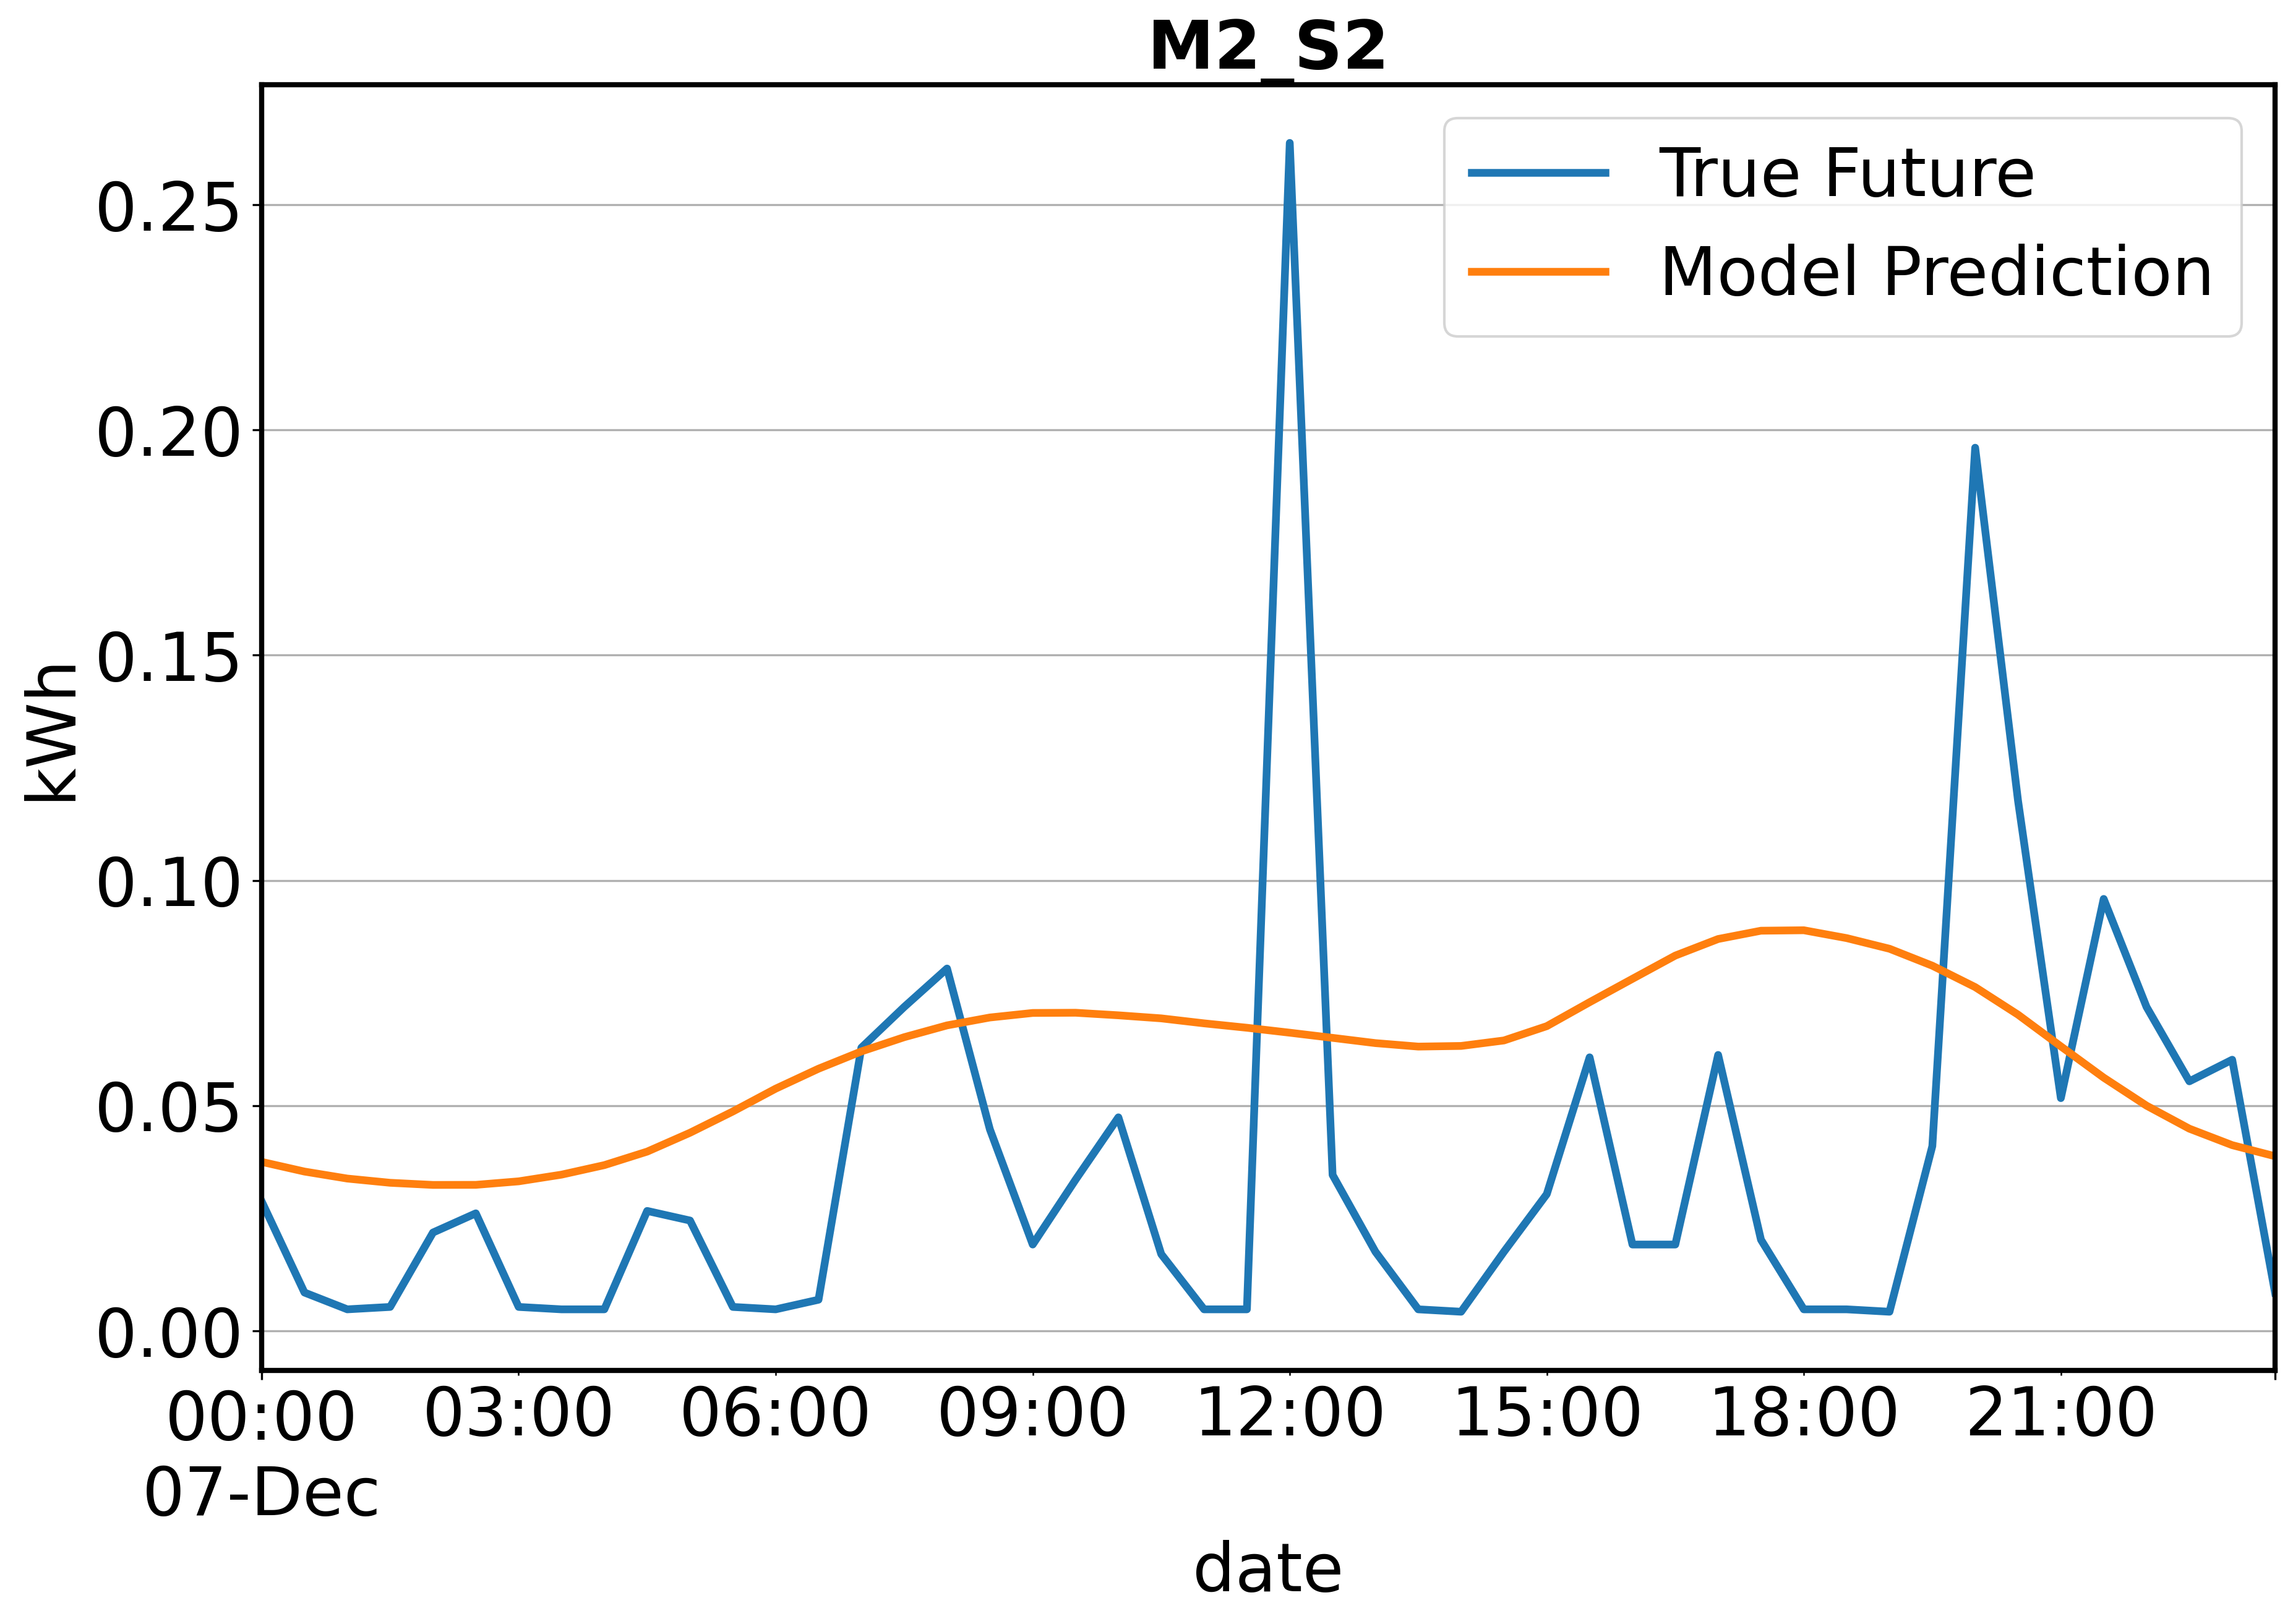
\includegraphics[width=1\linewidth]{IDM2_S2_Day341.png}
	 	\caption{Model $ 2 $ - Serie $ 2 $}
	 \end{subfigure}	
	 \begin{subfigure}{0.32\textwidth}
	 	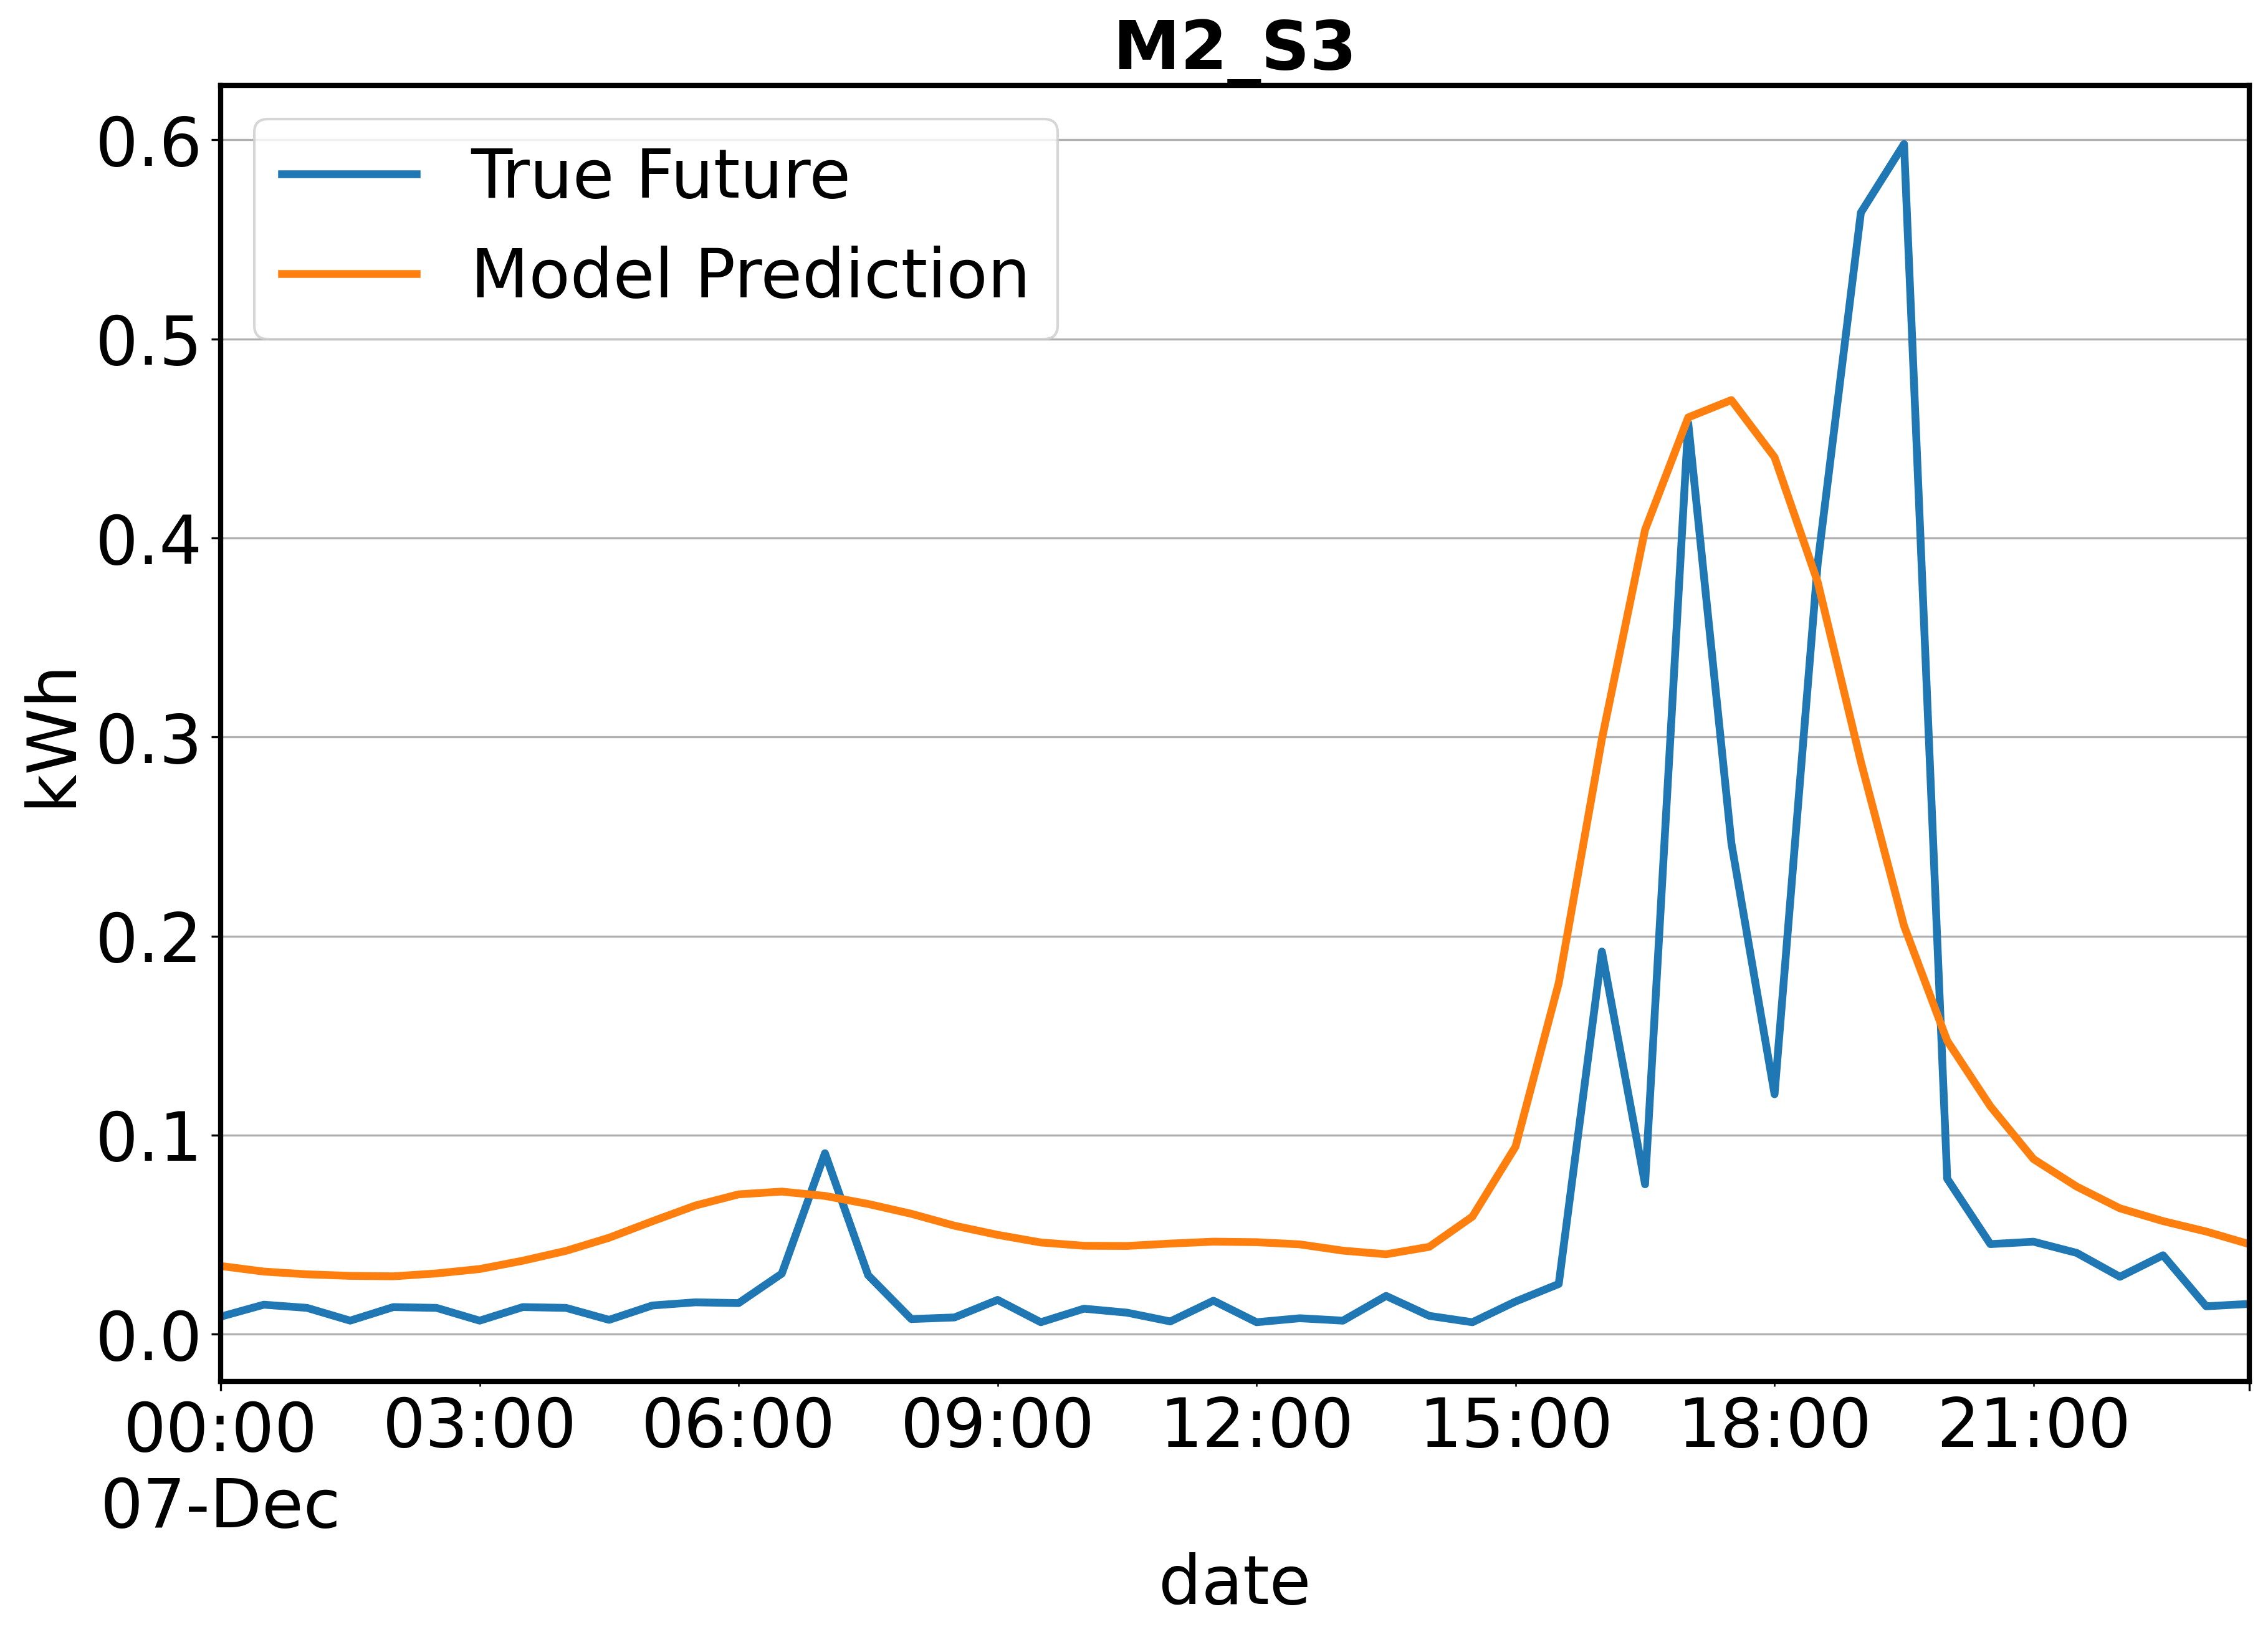
\includegraphics[width=1\linewidth]{IDM2_S3_Day341.png}
	 	\caption{Model $ 2 $ - Serie $ 3 $}
	 \end{subfigure}
 	\begin{subfigure}{0.32\textwidth}
	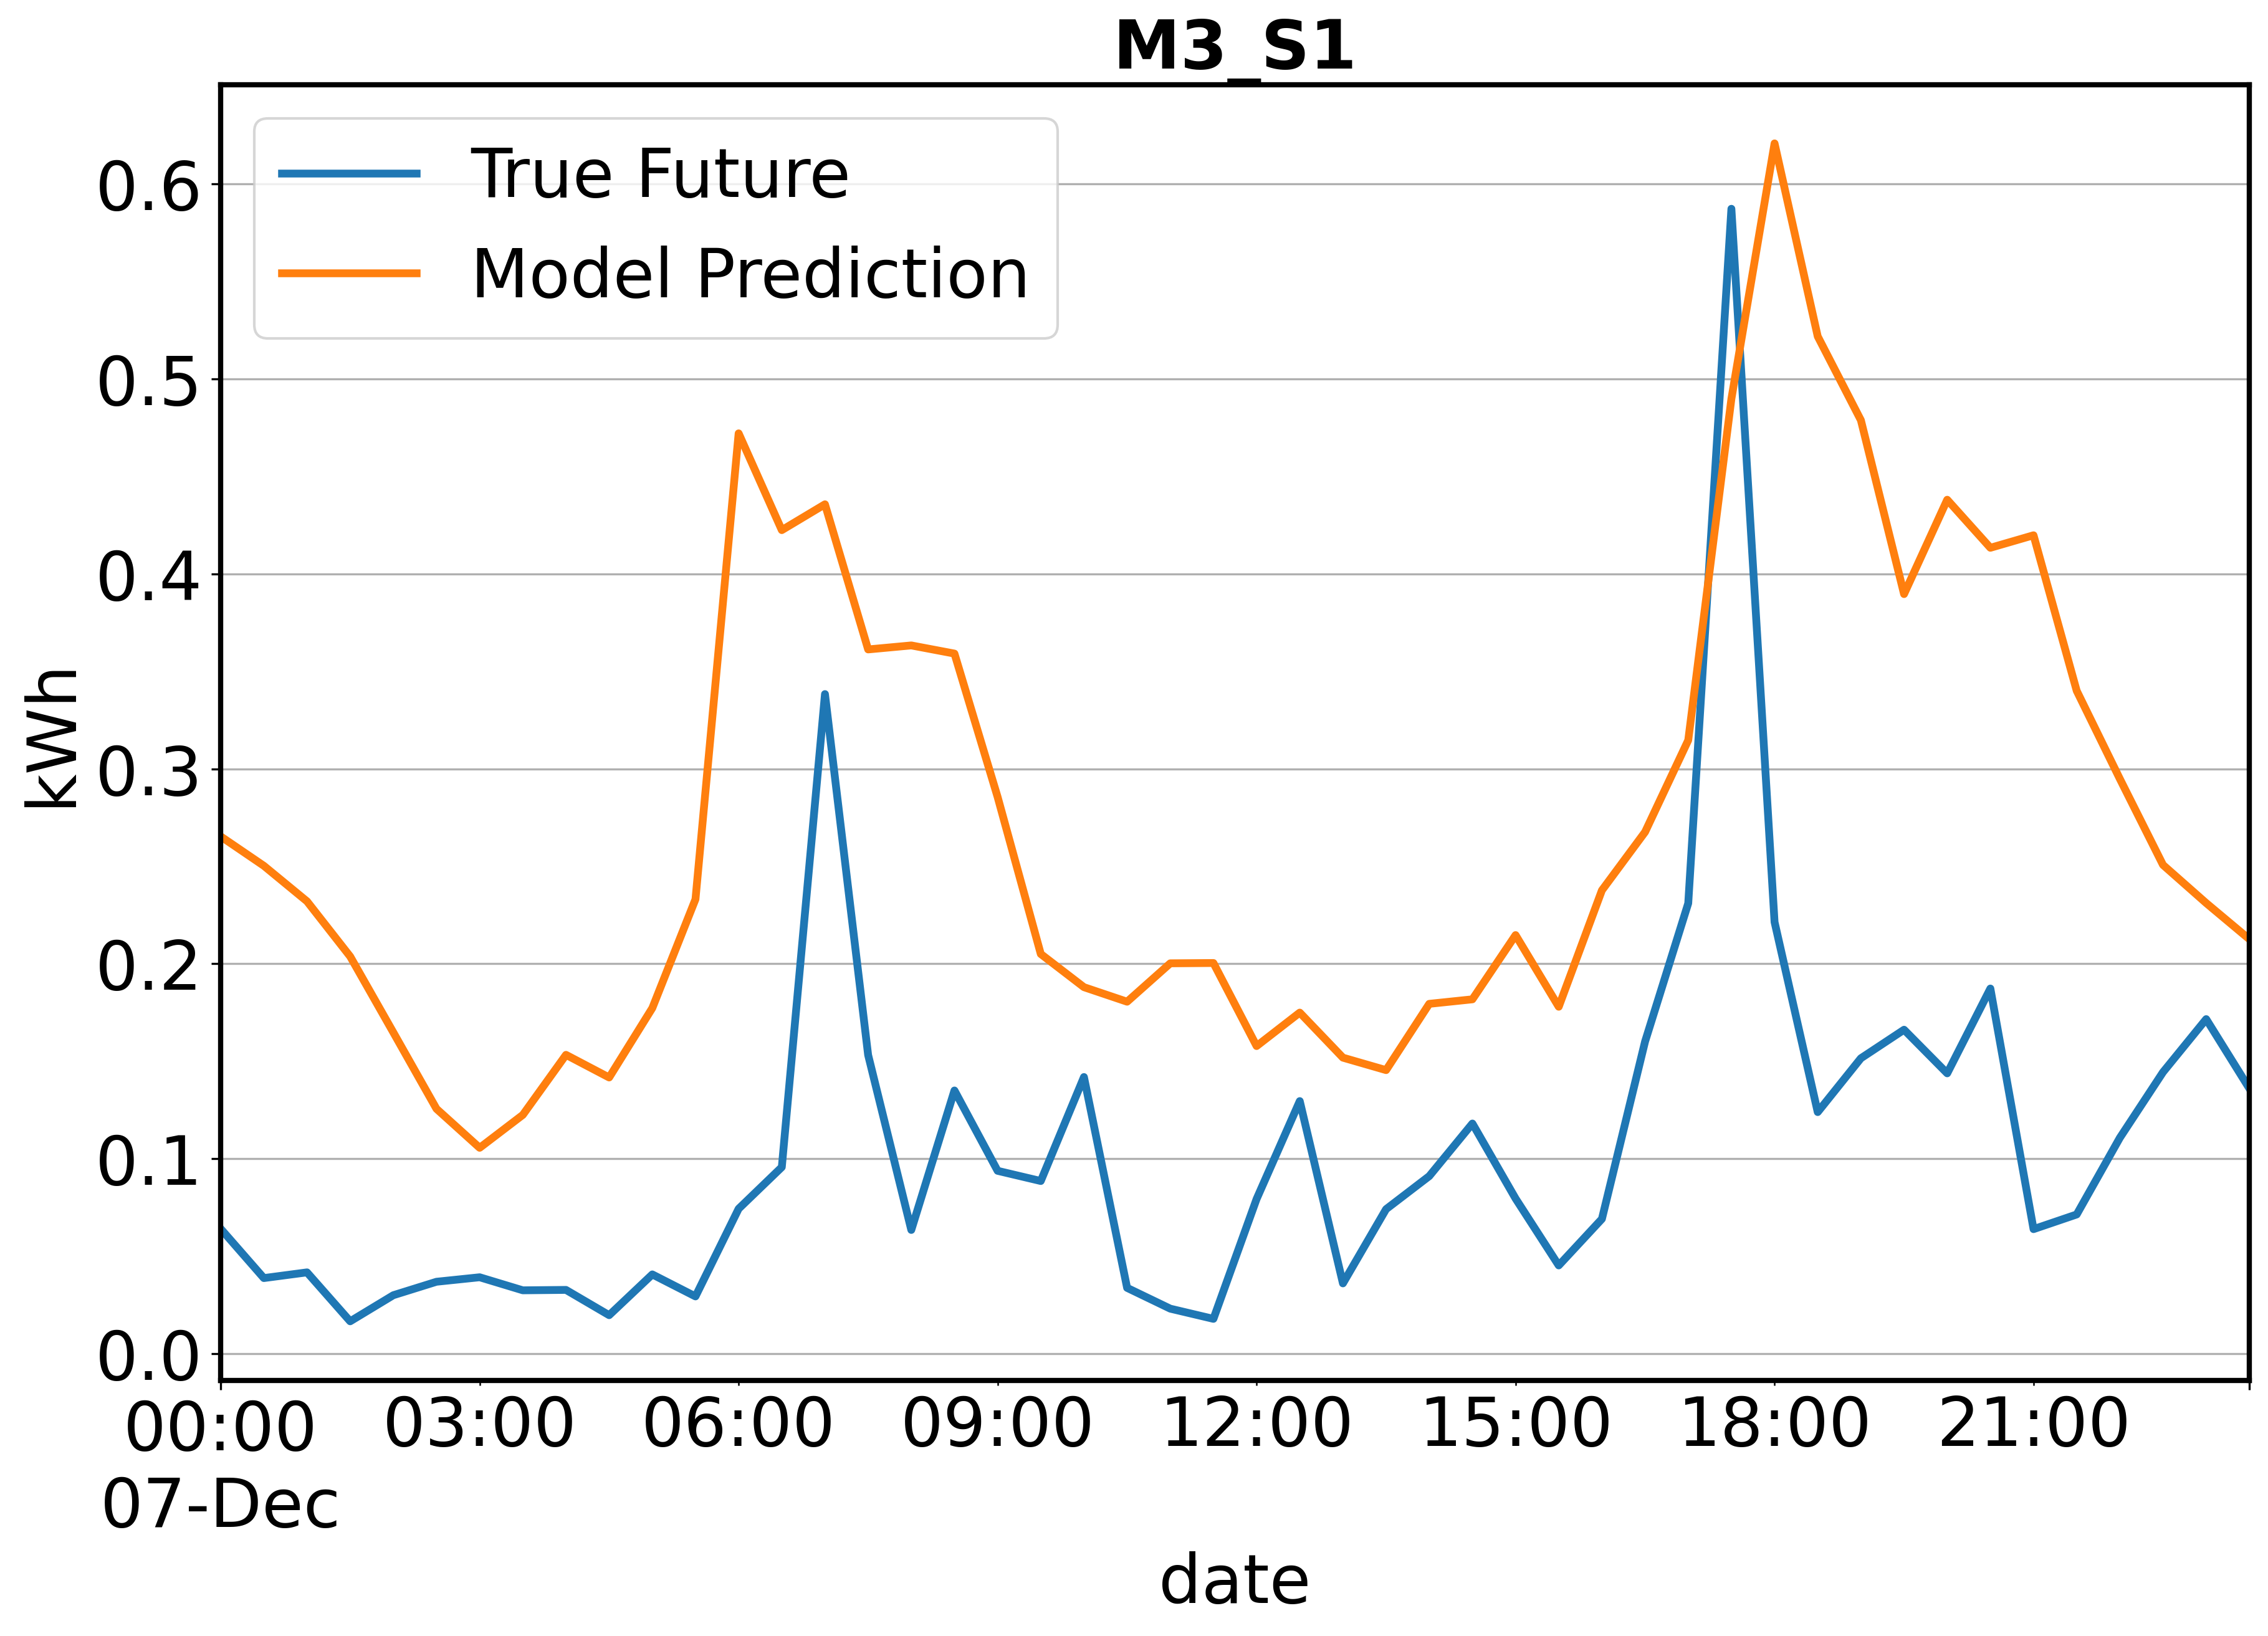
\includegraphics[width=1\linewidth]{IDM3_S1_Day341.png}
	\caption{Model $3 $ - Serie $ 1 $}
	\end{subfigure}	 	
	\begin{subfigure}{0.32\textwidth}
		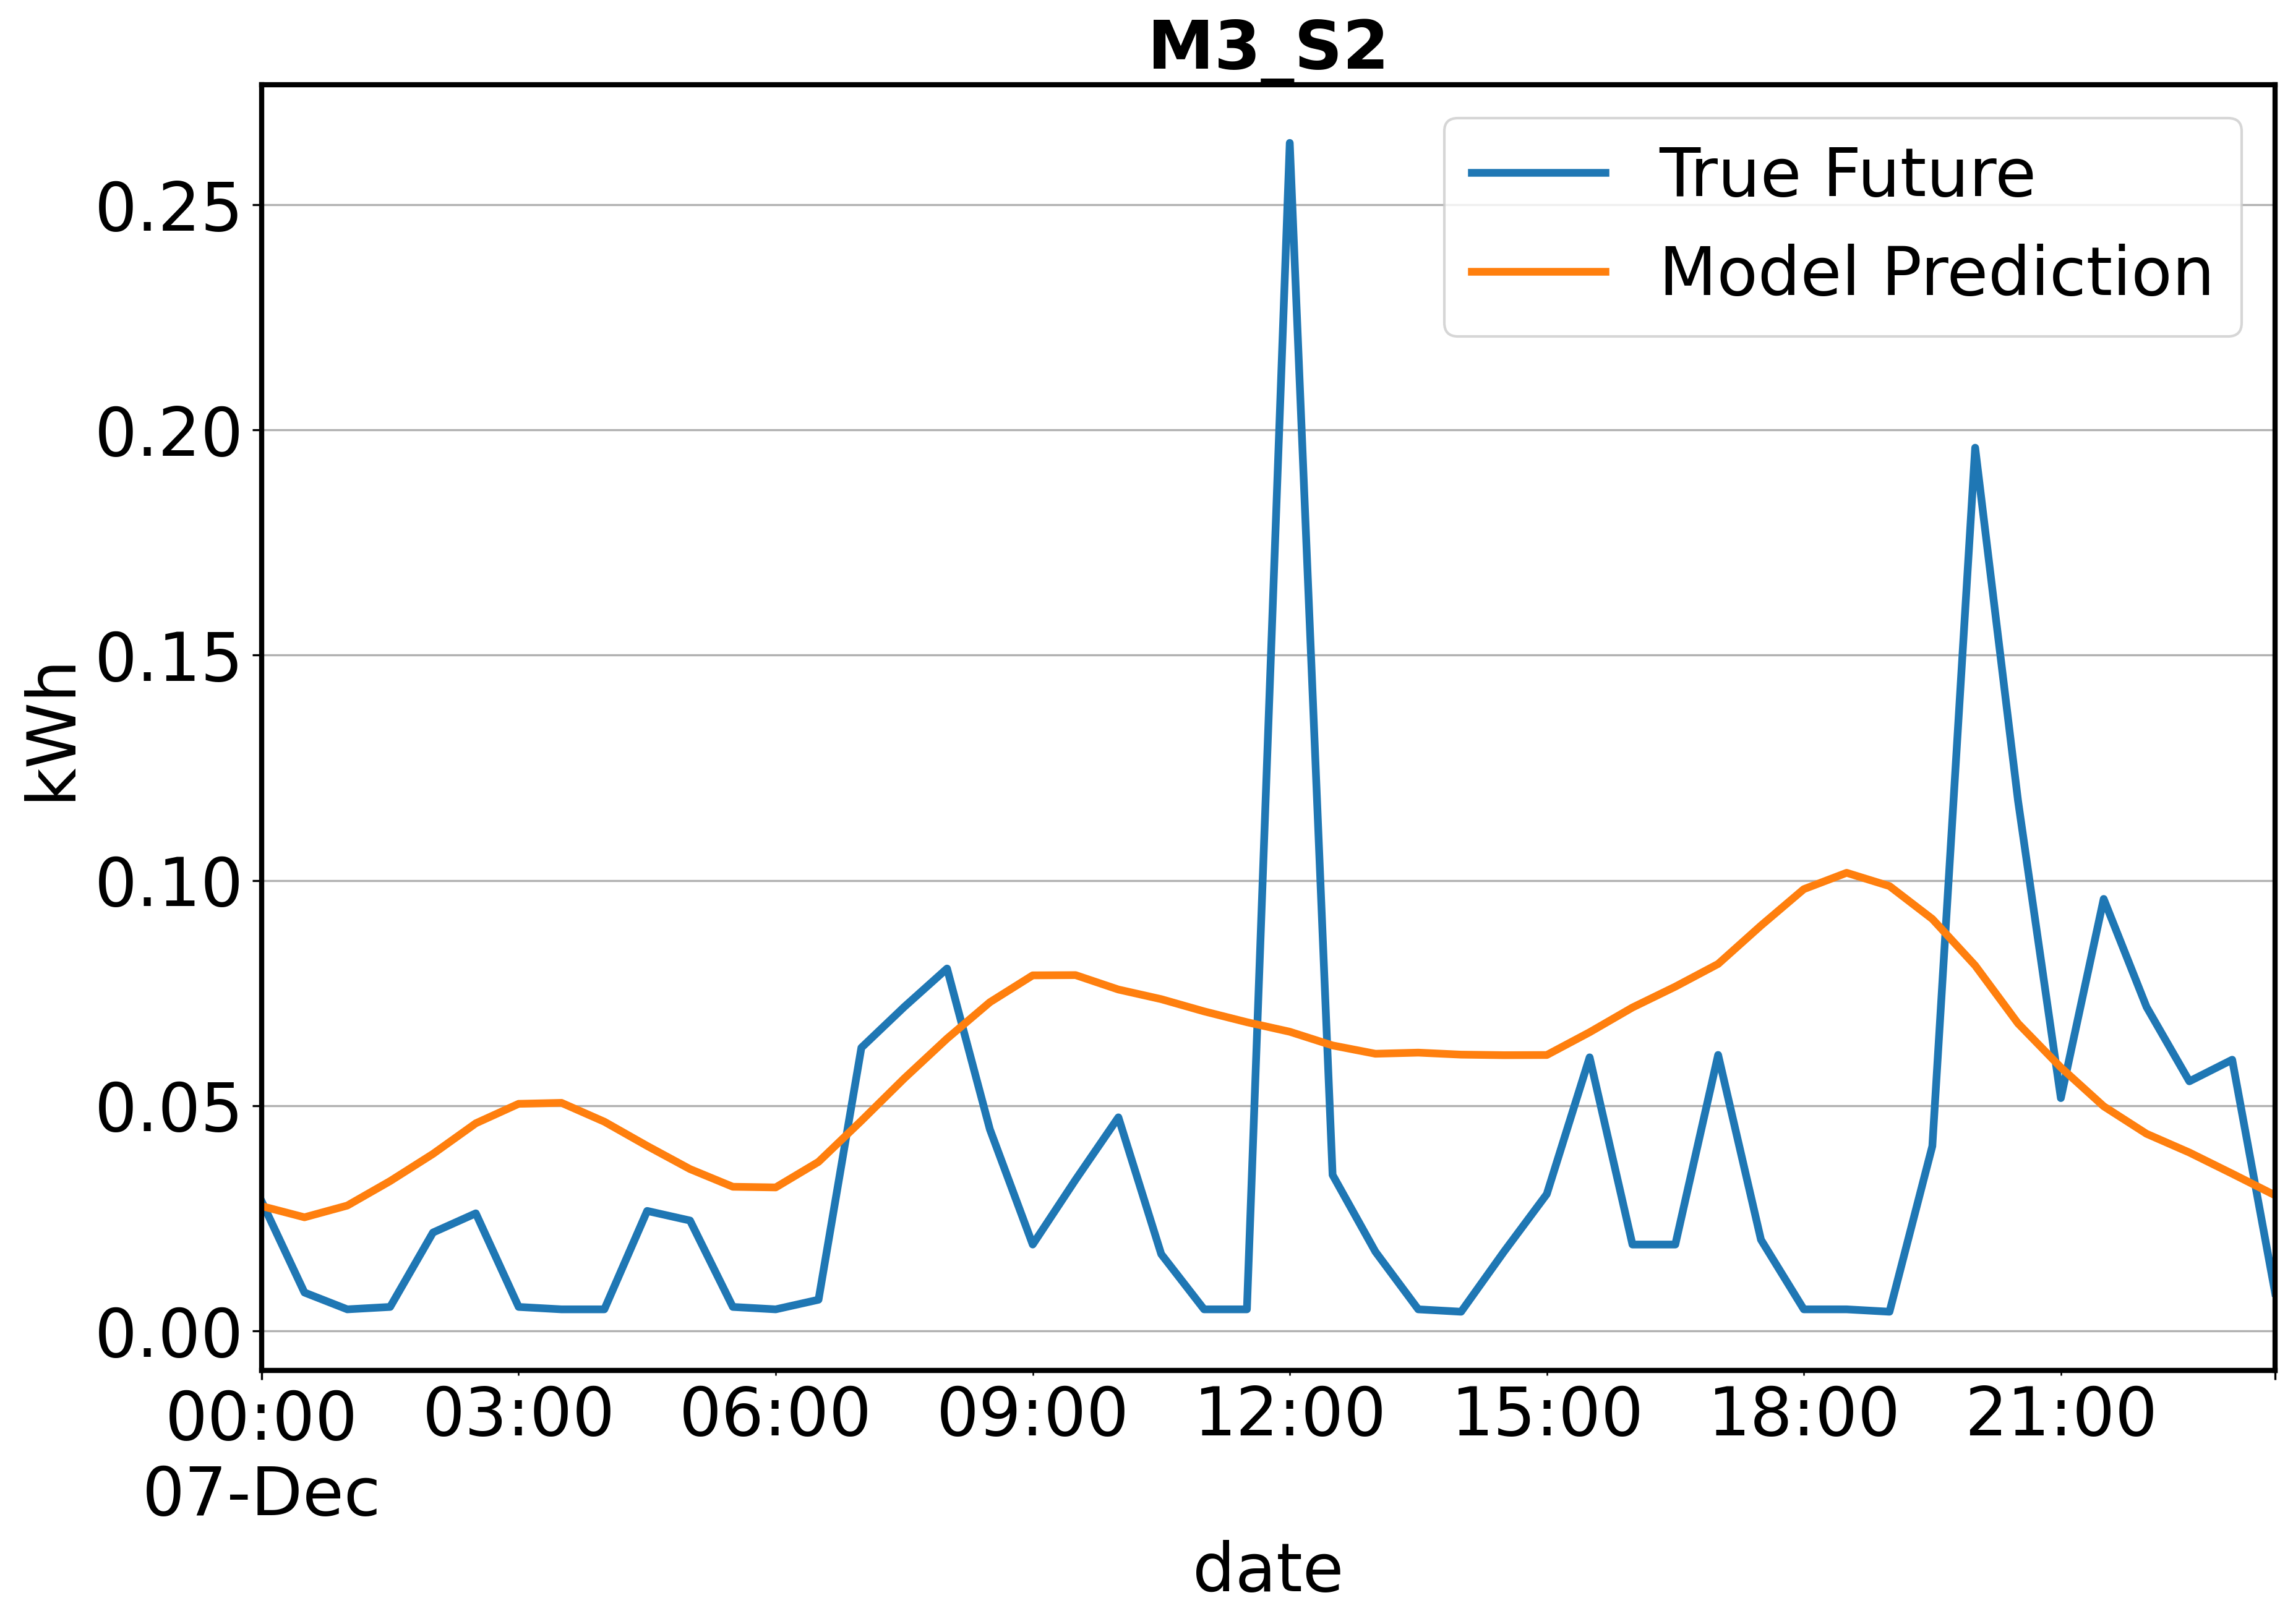
\includegraphics[width=1\linewidth]{IDM3_S2_Day341.png}
		\caption{Model $3 $ - Serie $ 2 $}
	\end{subfigure}	
	\begin{subfigure}{0.32\textwidth}
		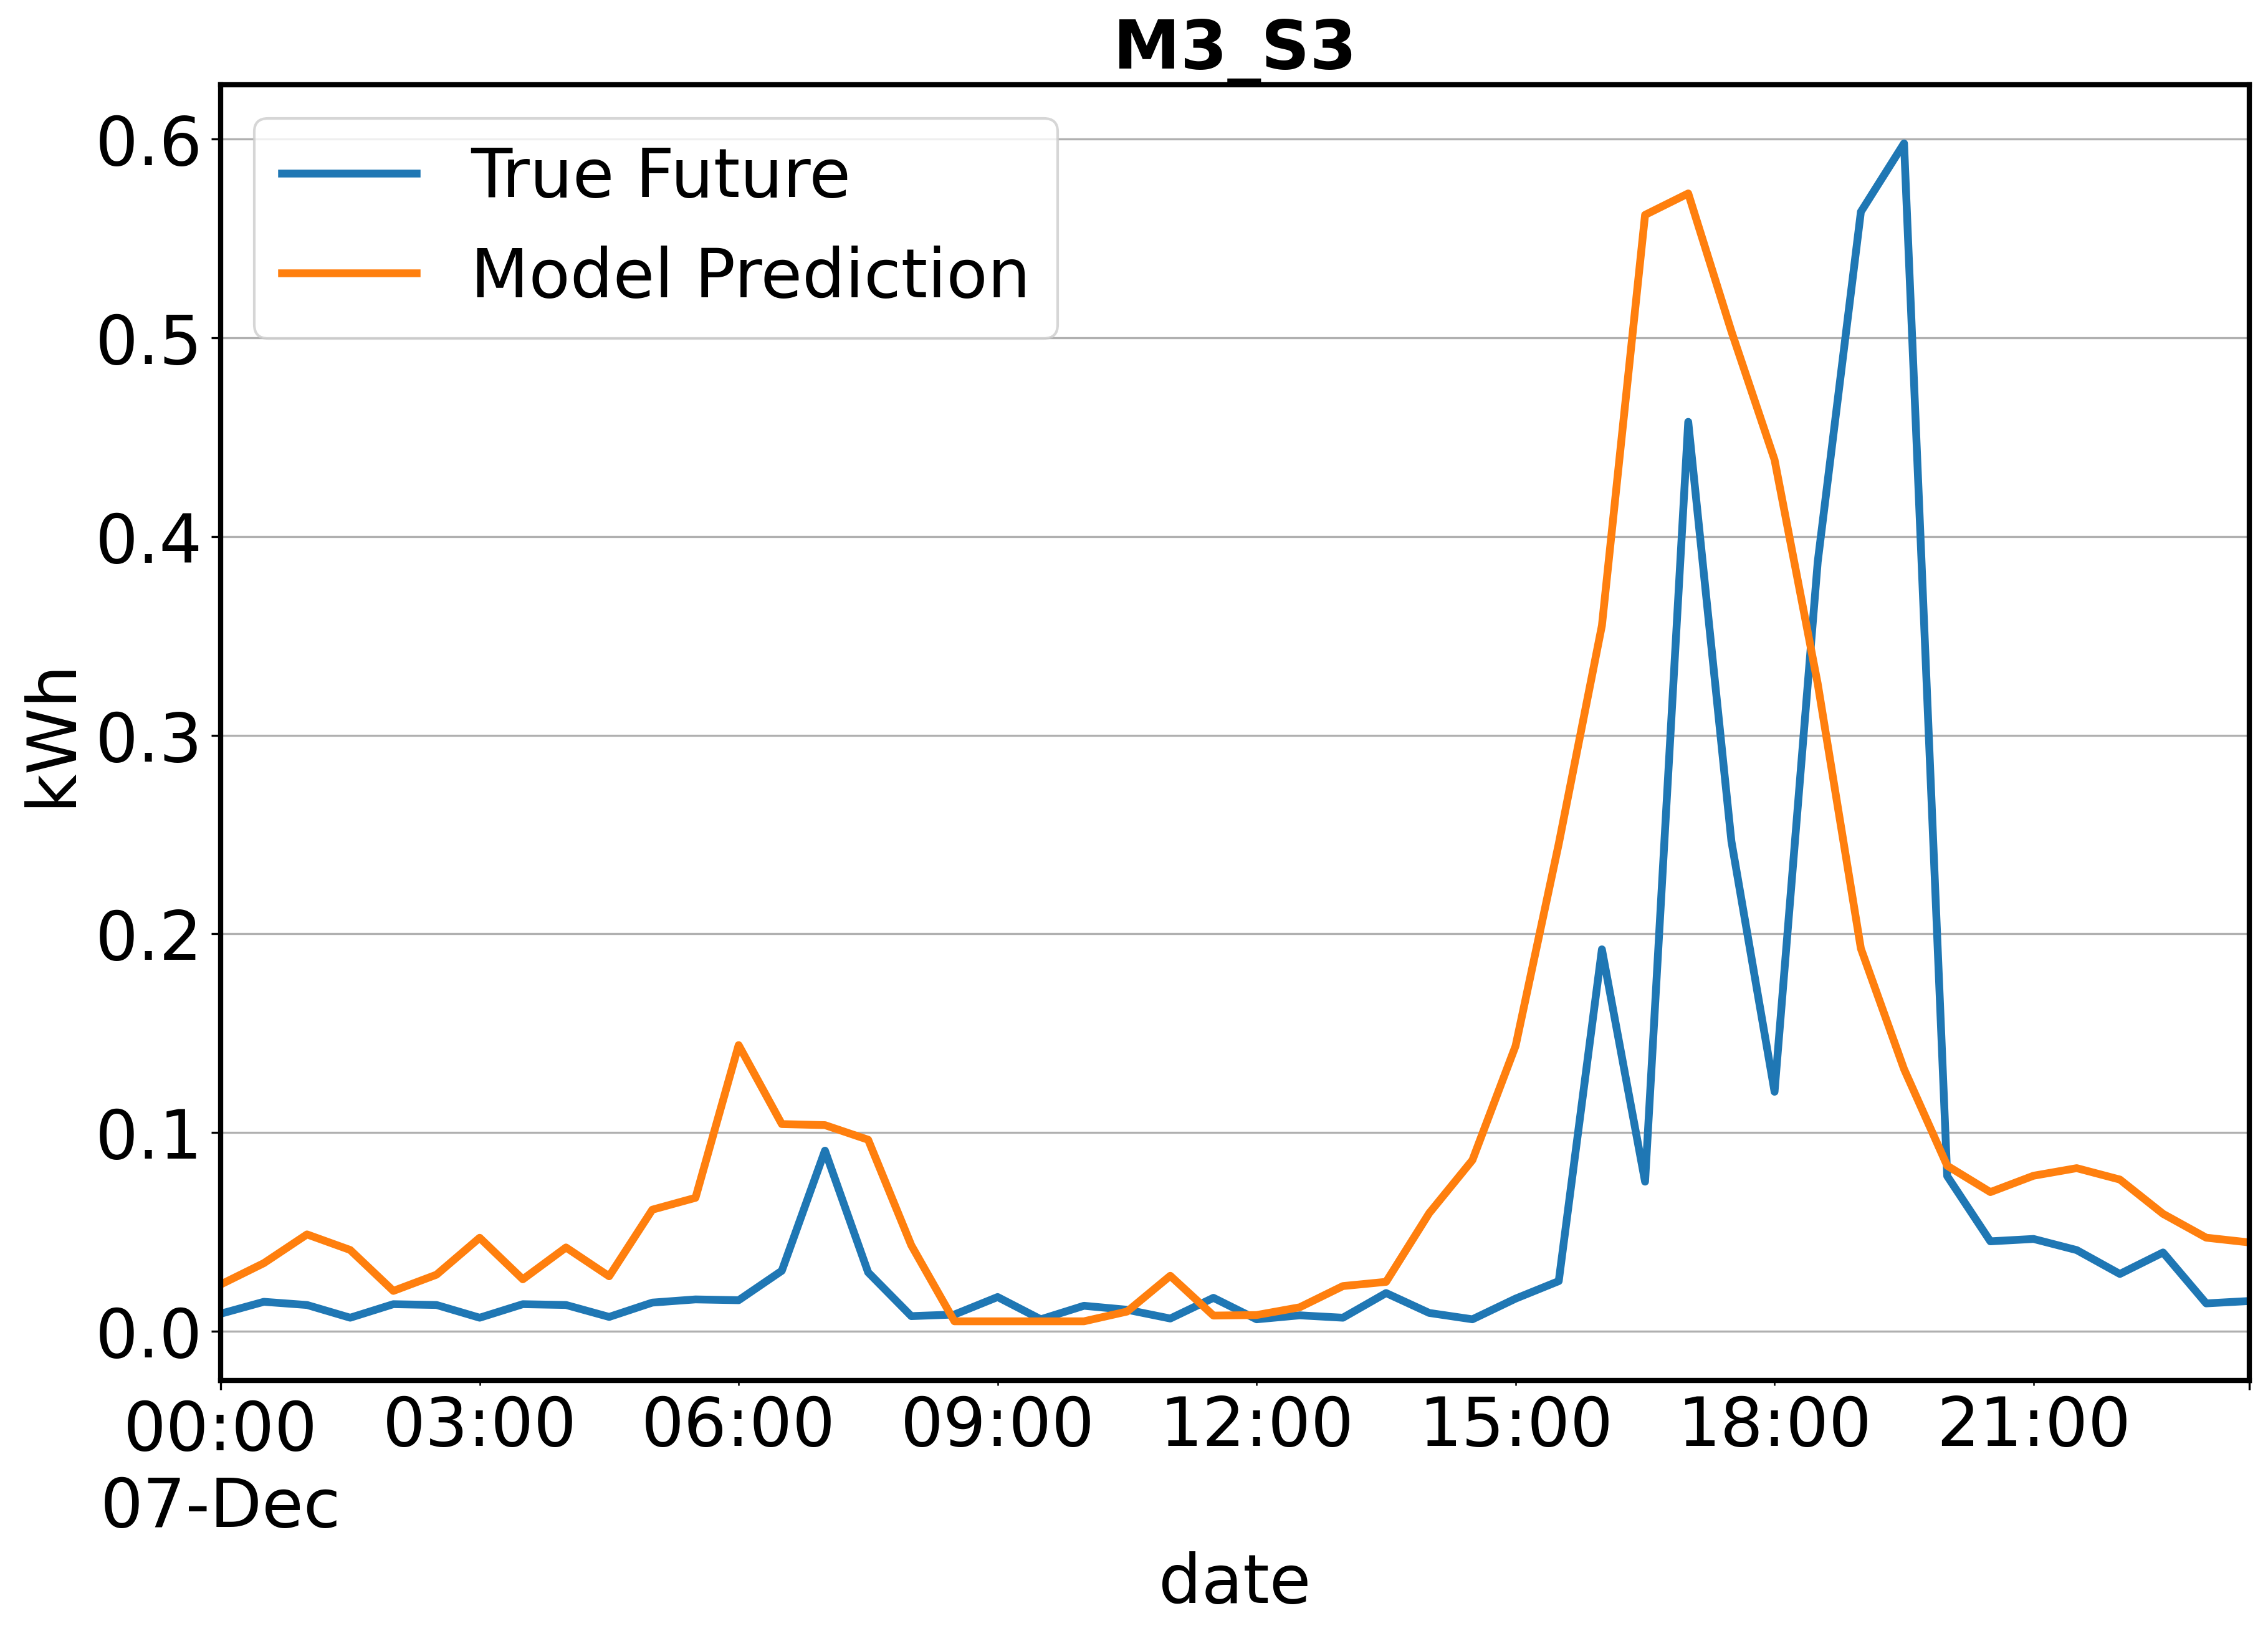
\includegraphics[width=1\linewidth]{IDM3_S3_Day341.png}
		\caption{Model $3 $ - Serie $ 3 $}
	\end{subfigure}
 	\begin{subfigure}{0.32\textwidth}
		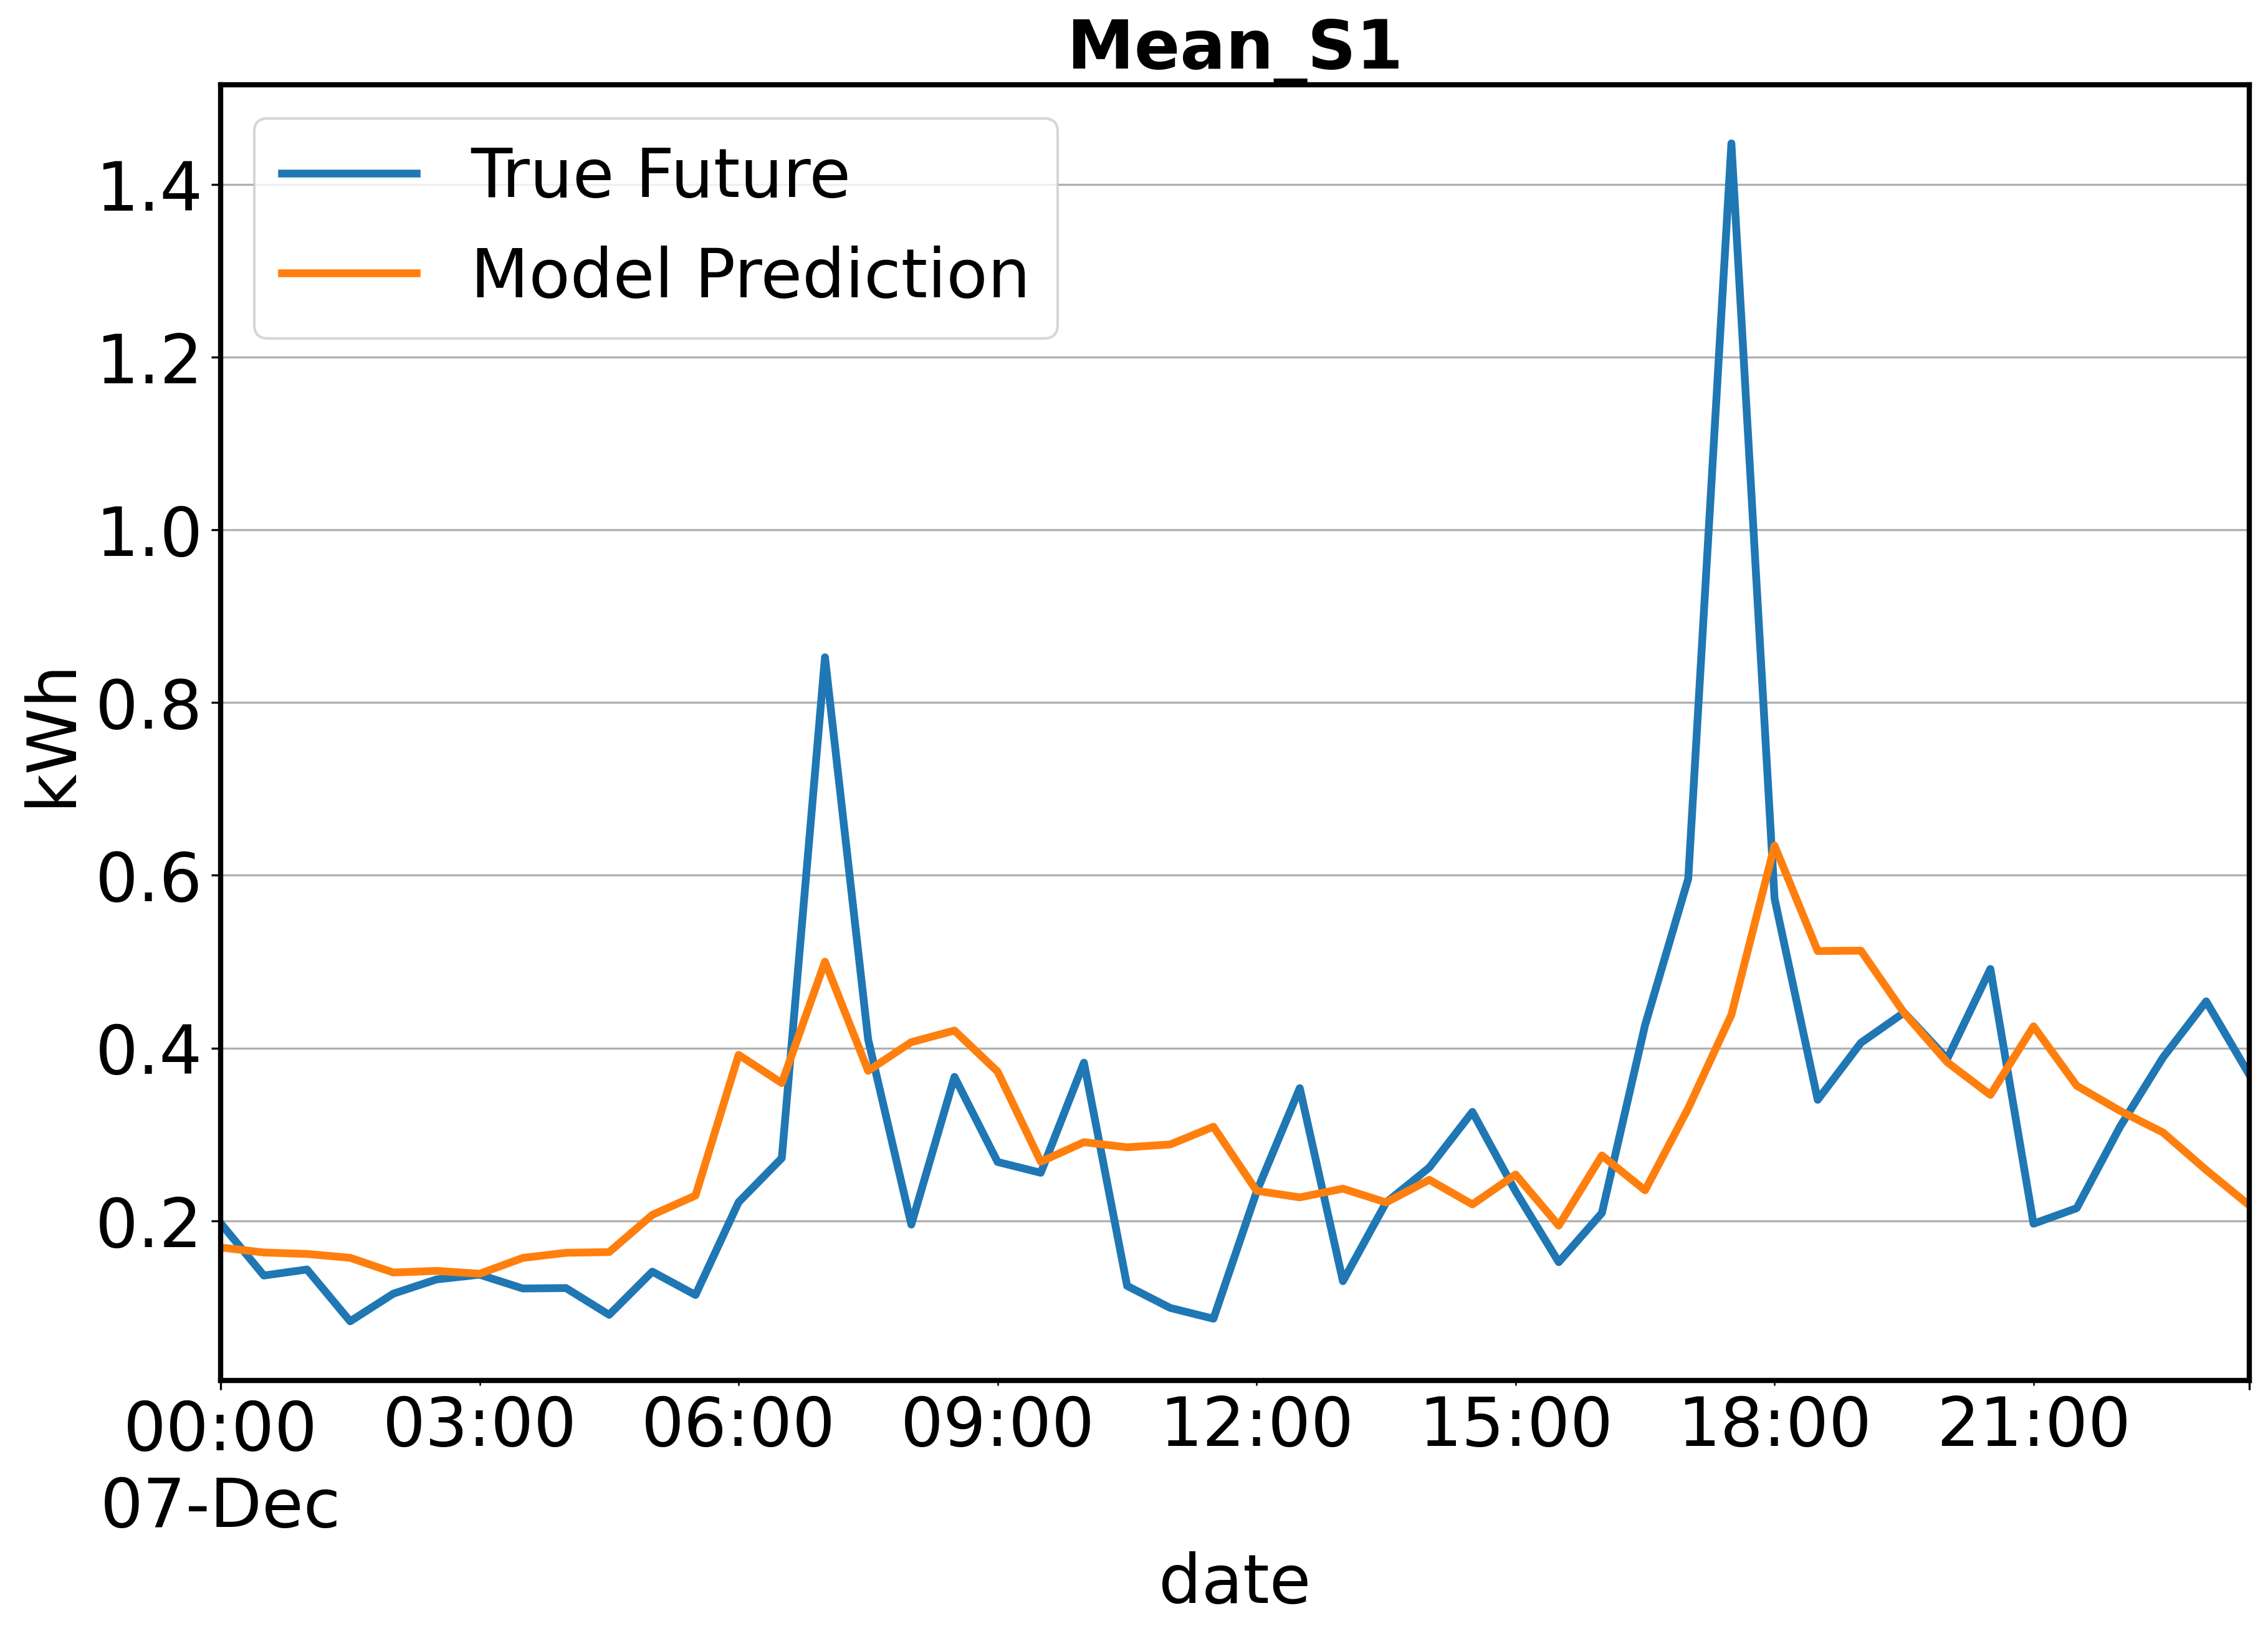
\includegraphics[width=1\linewidth]{IDMean_S1_Day341.png}
		\caption{Mean forecast - Serie $ 1 $}
	\end{subfigure}	 	
	\begin{subfigure}{0.32\textwidth}
		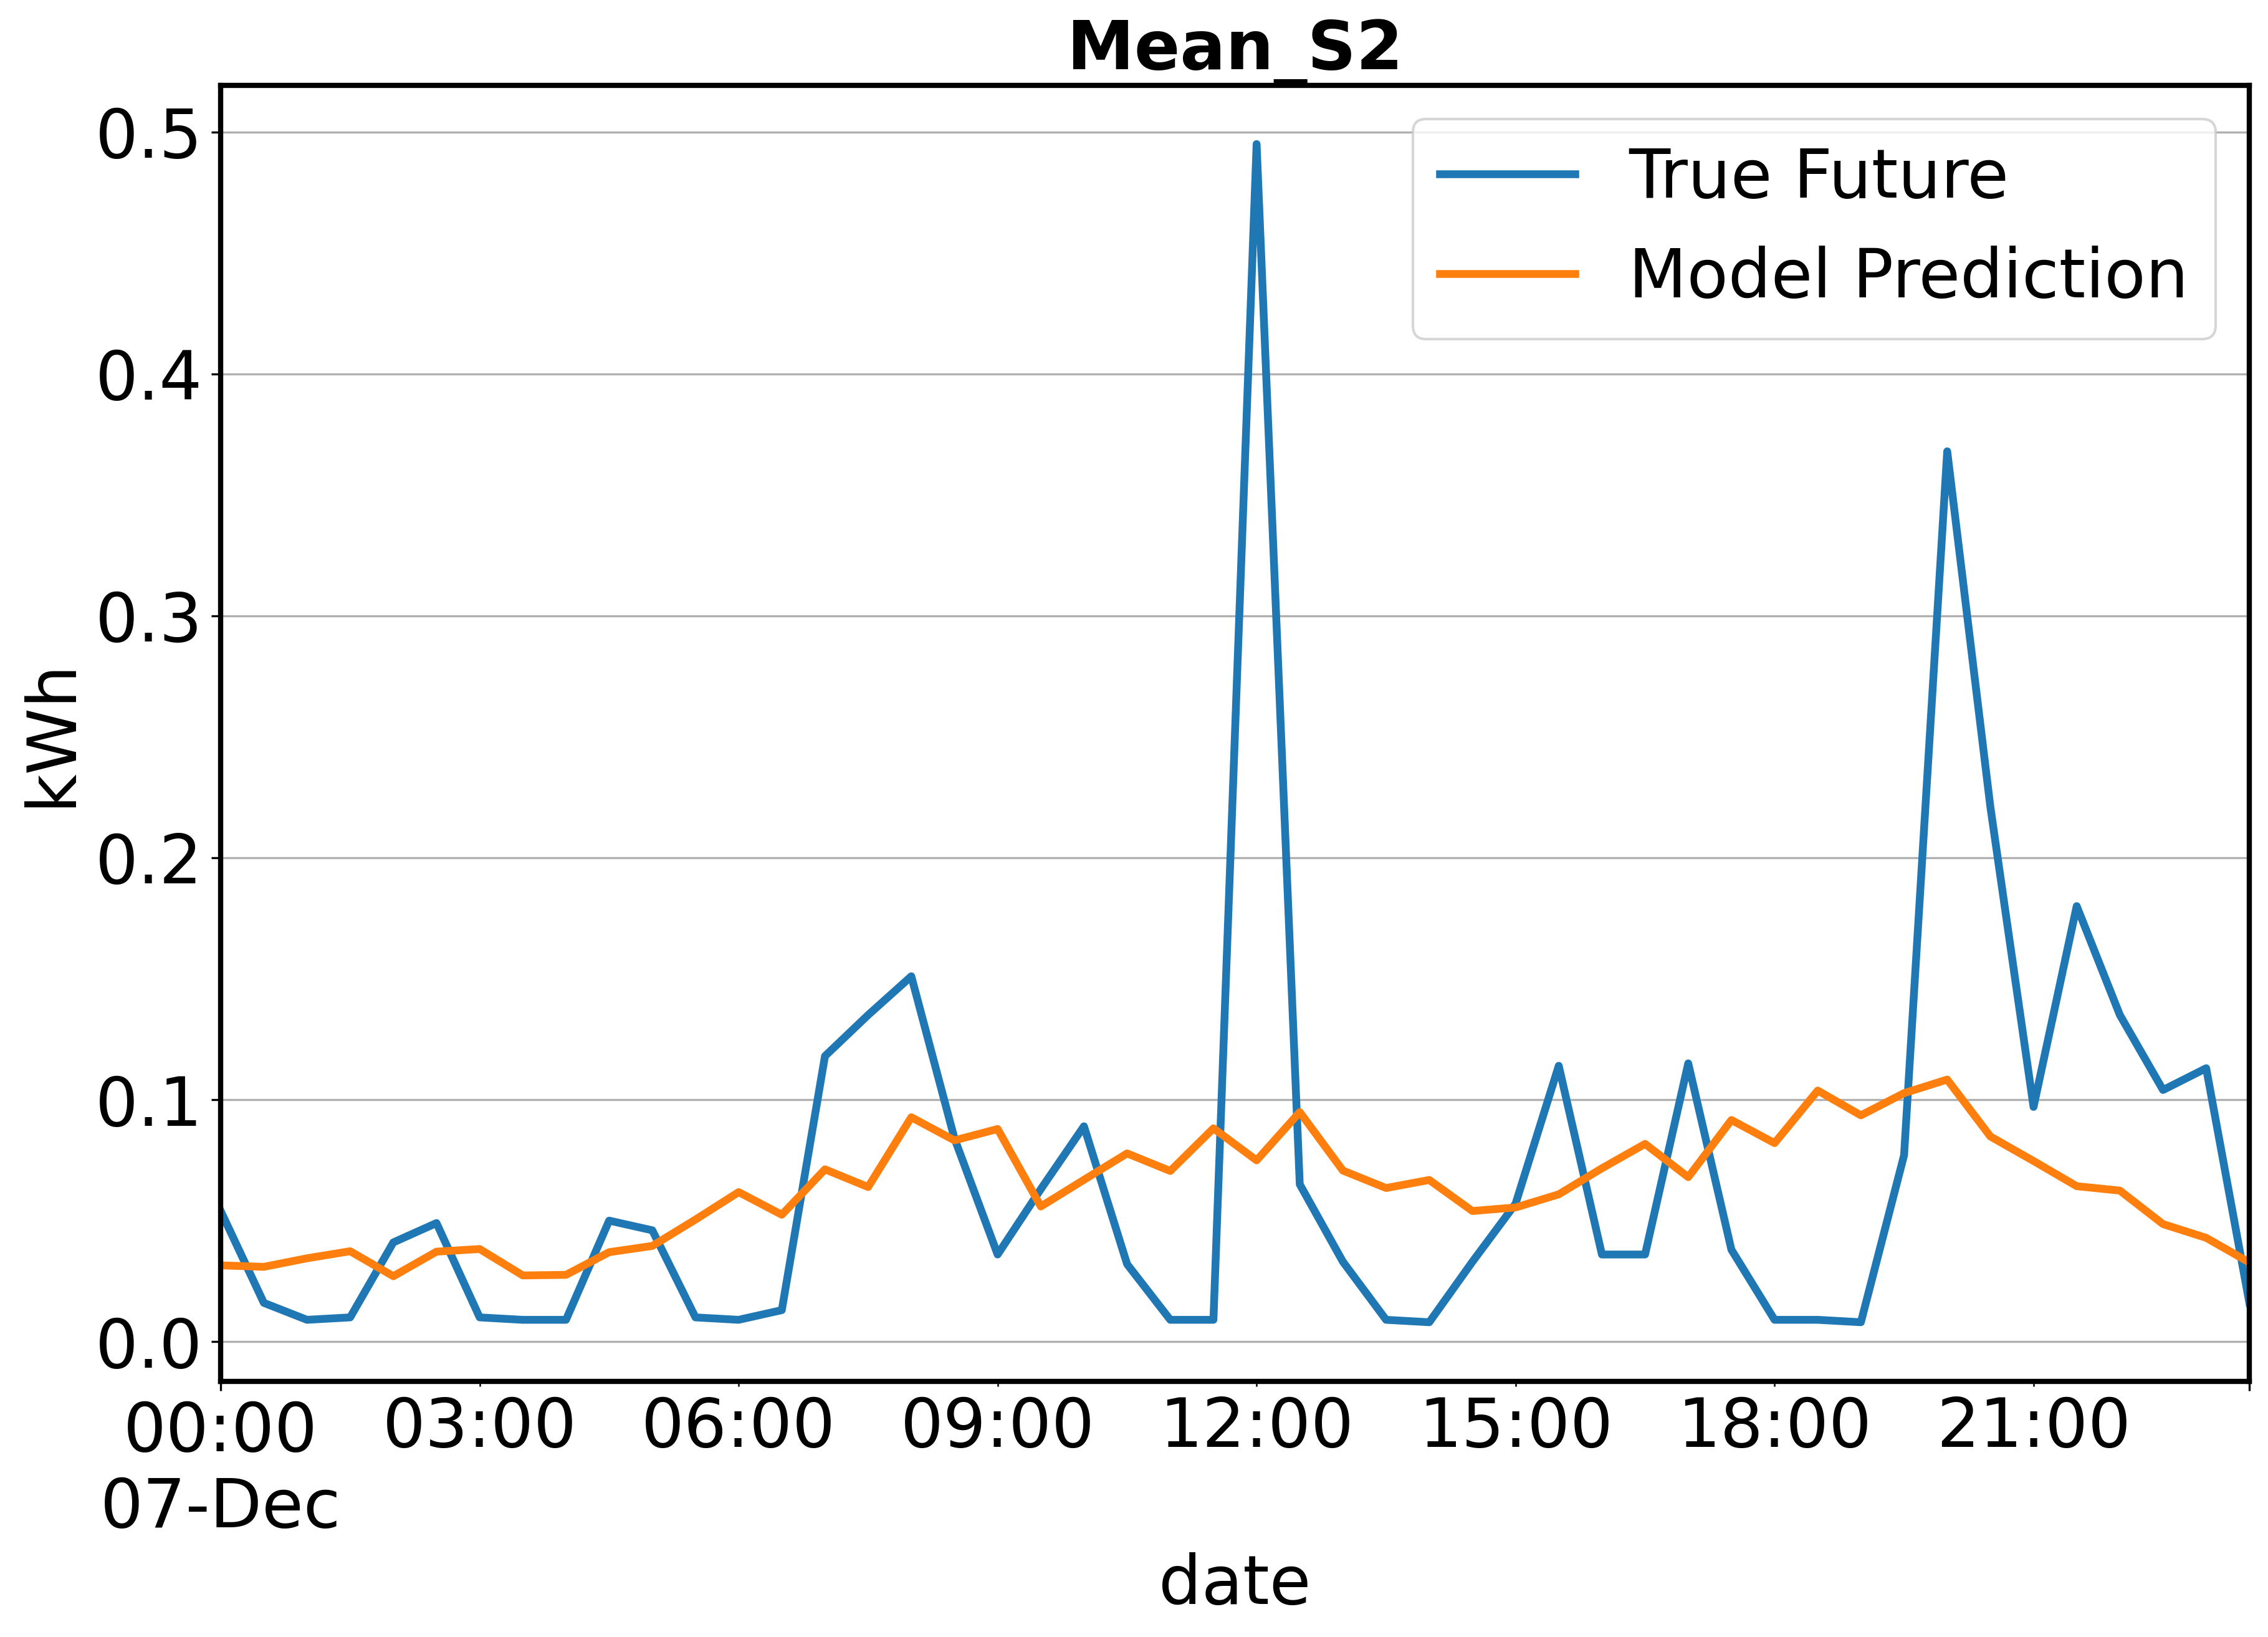
\includegraphics[width=1\linewidth]{IDMean_S2_Day341.png}
		\caption{Mean forecast - Serie $ 2 $}
	\end{subfigure}	
	\begin{subfigure}{0.32\textwidth}
		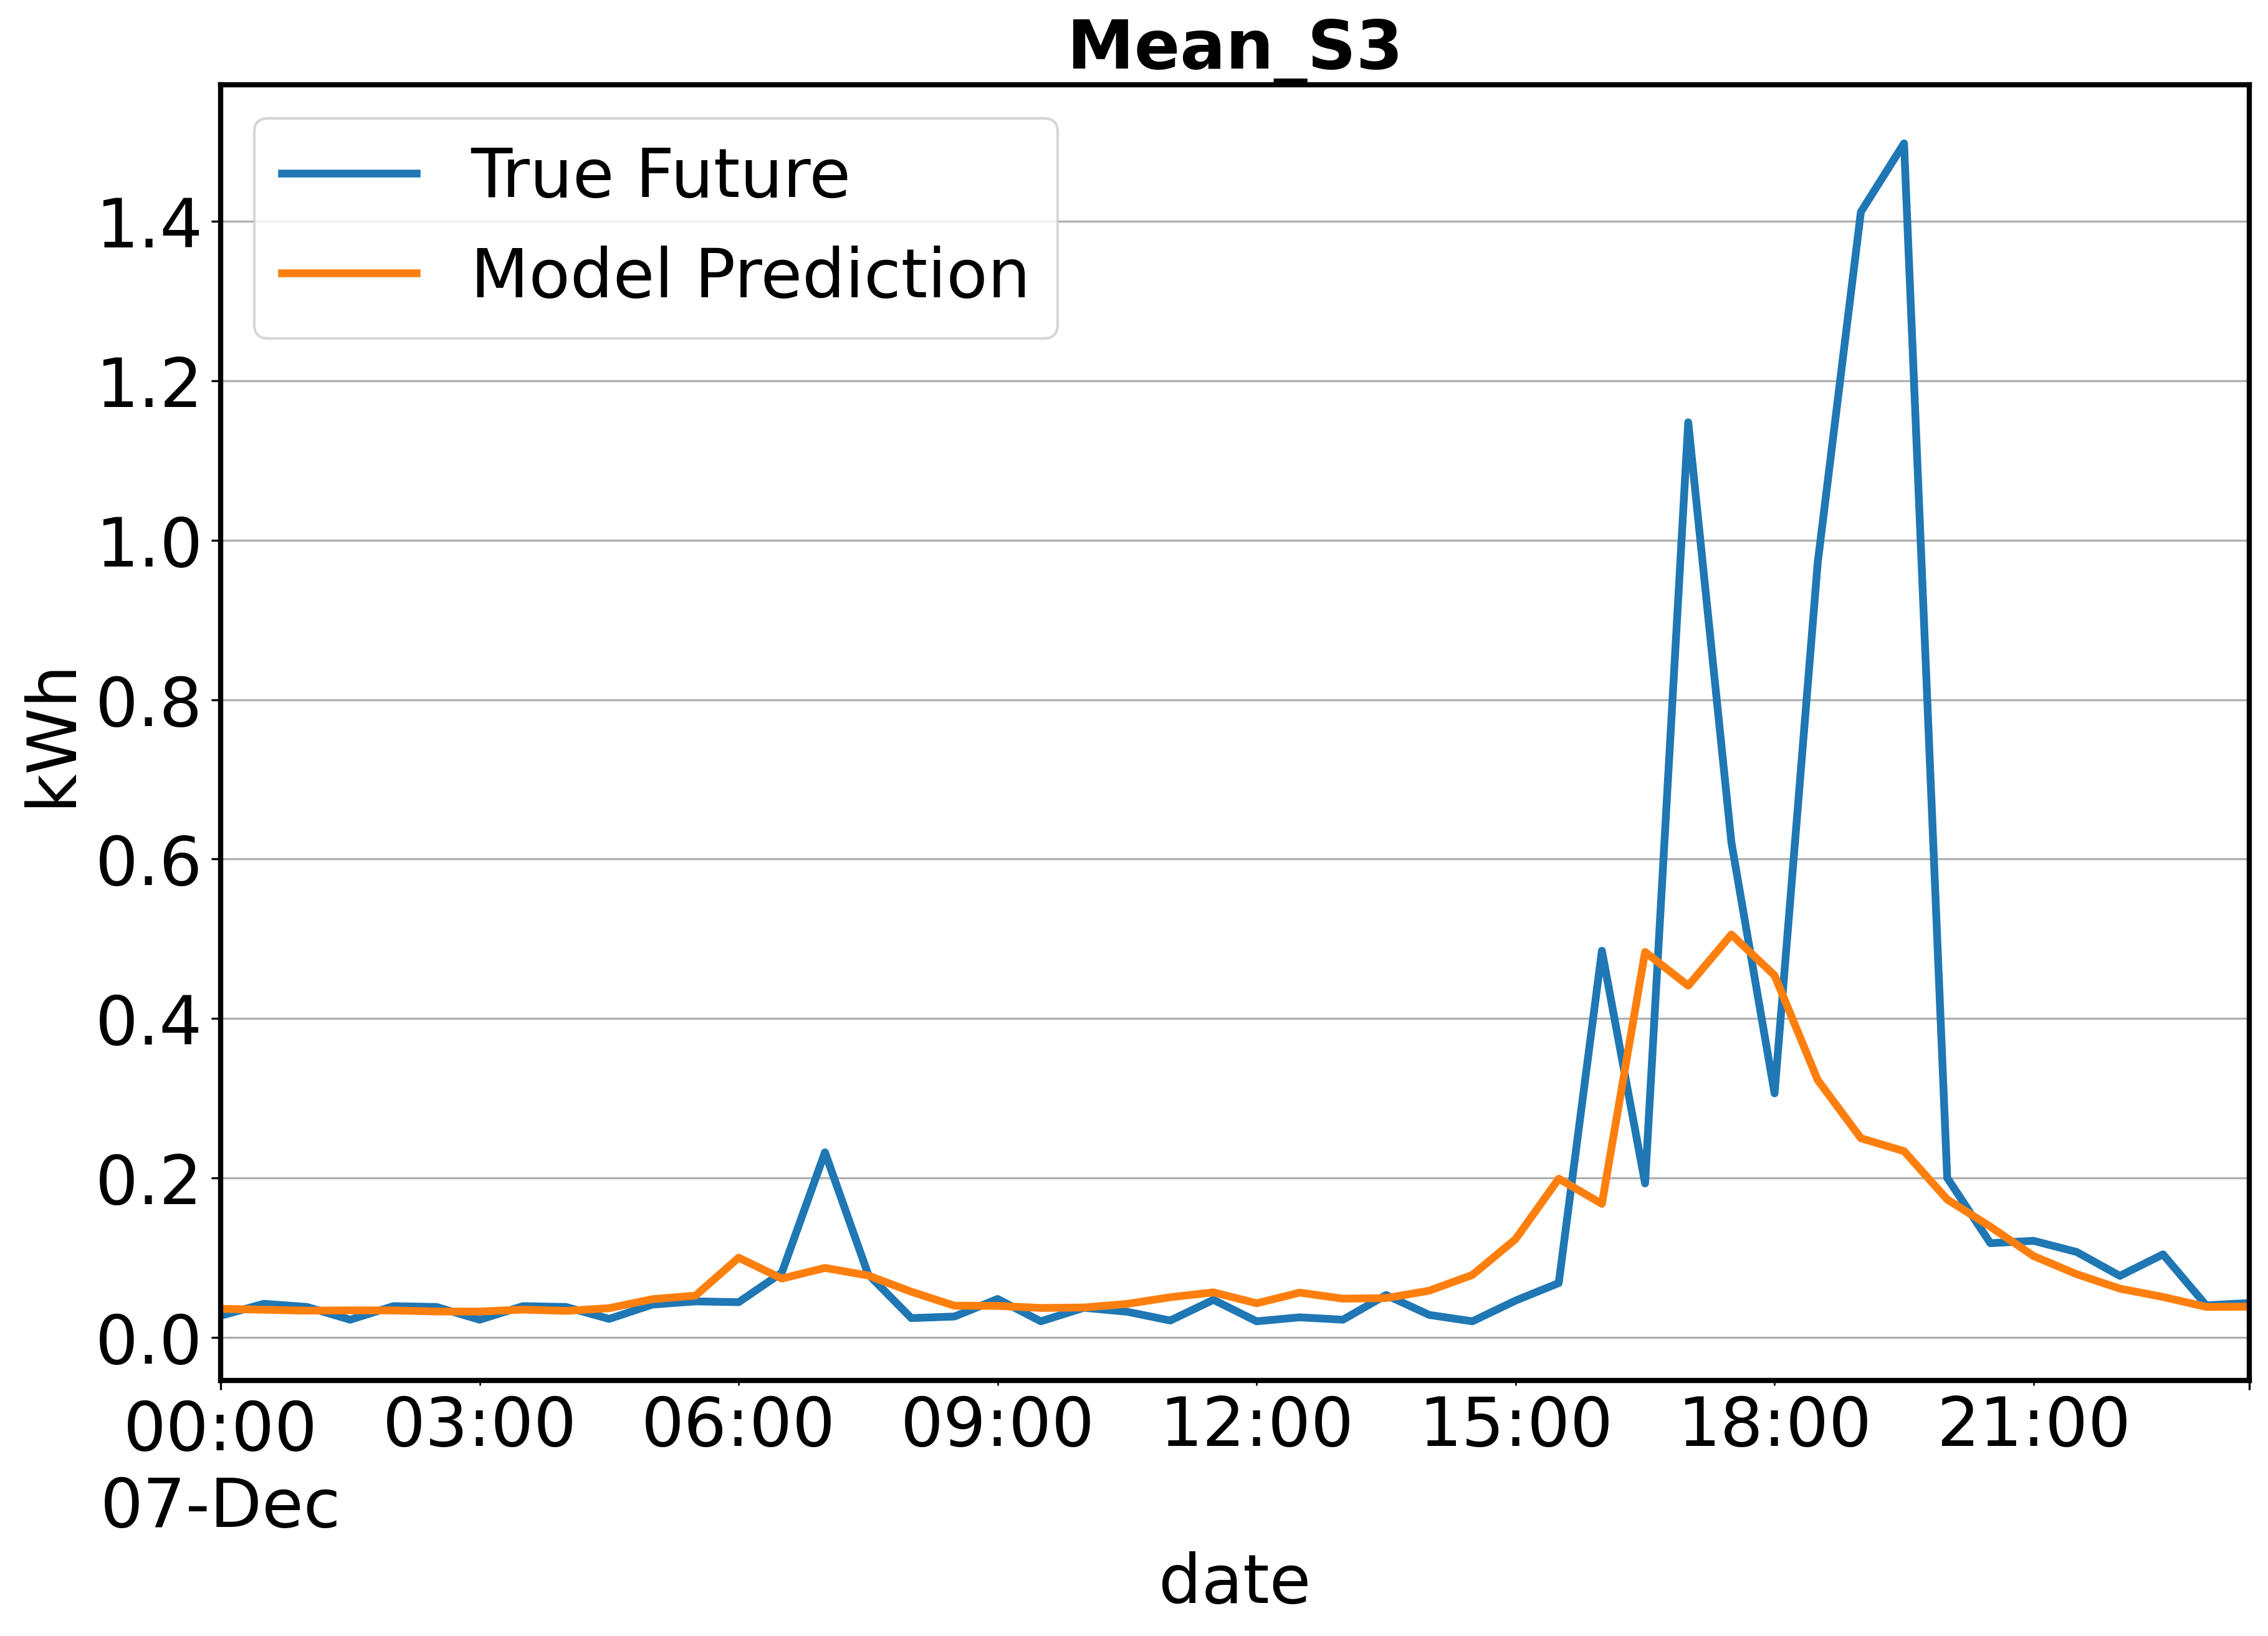
\includegraphics[width=1\linewidth]{IDMean_S3_Day341.png}
		\caption{Mean forecast - Serie $ 3 $}
	\end{subfigure}
	 \begin{subfigure}{0.32\textwidth}
		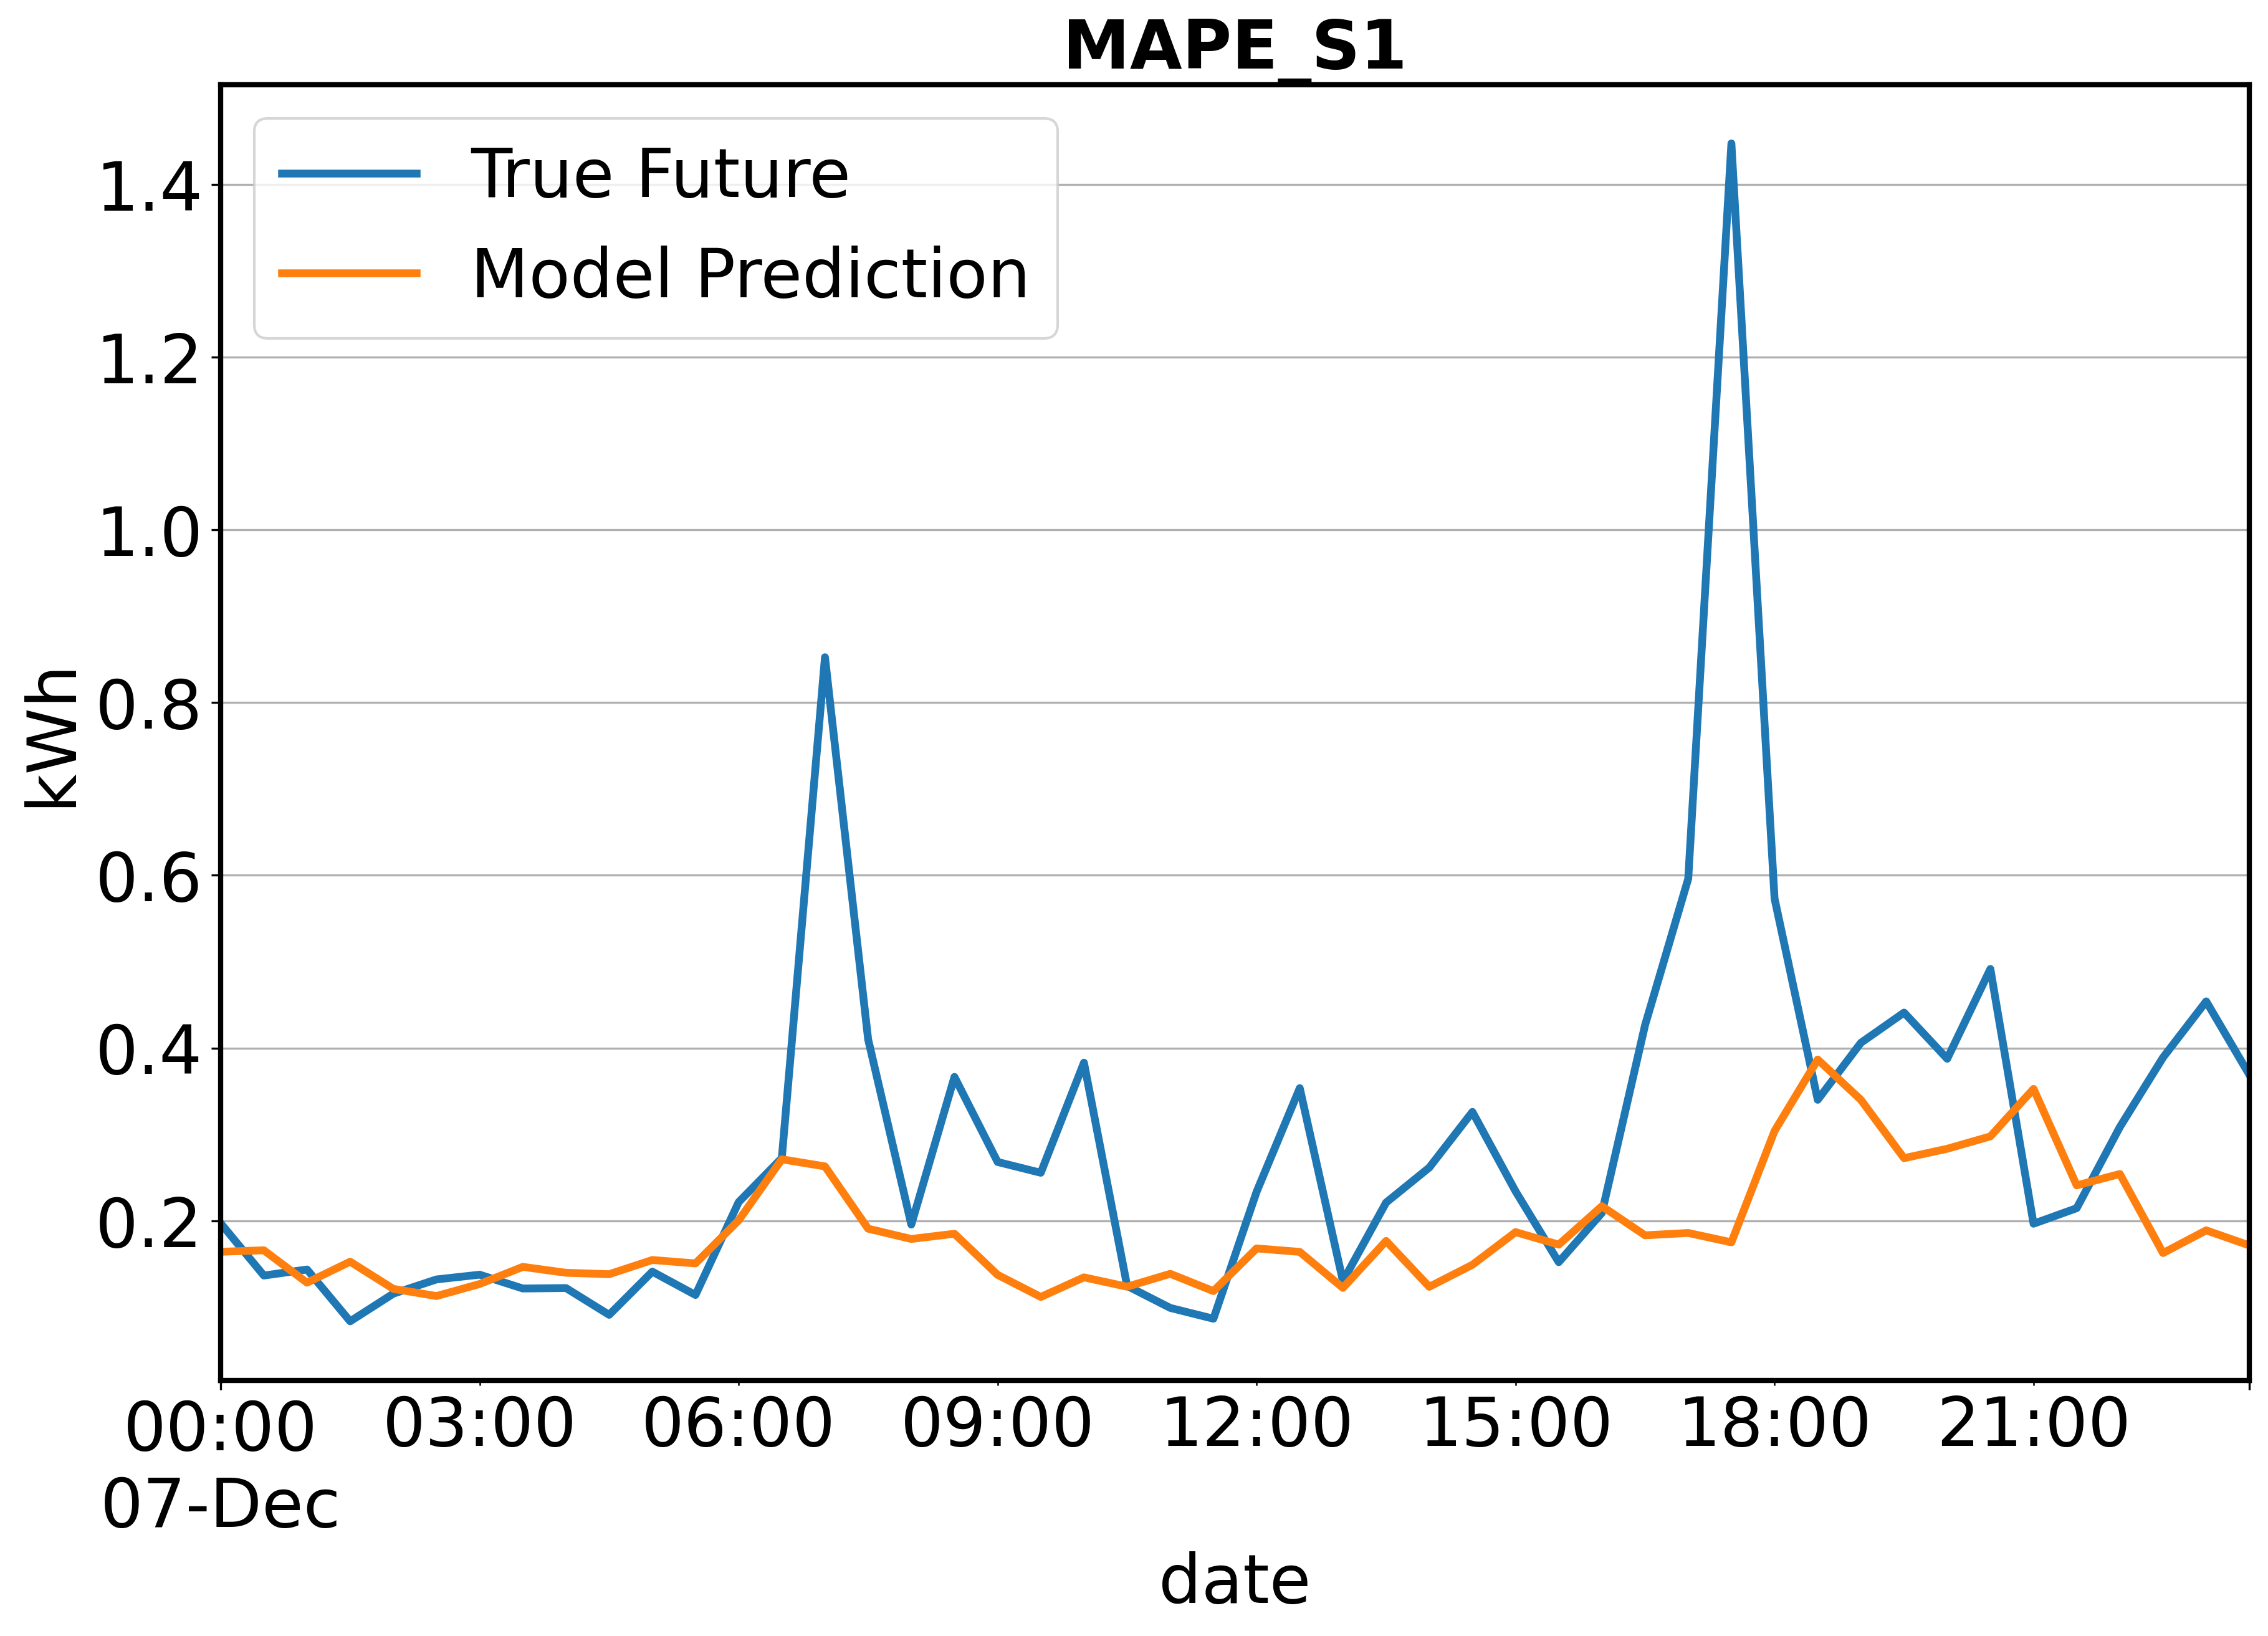
\includegraphics[width=1\linewidth]{IDMAPE_S1_Day341.png}
		\caption{MAPE forecast - Serie $ 1 $}
	\end{subfigure}	 	
	\begin{subfigure}{0.32\textwidth}
		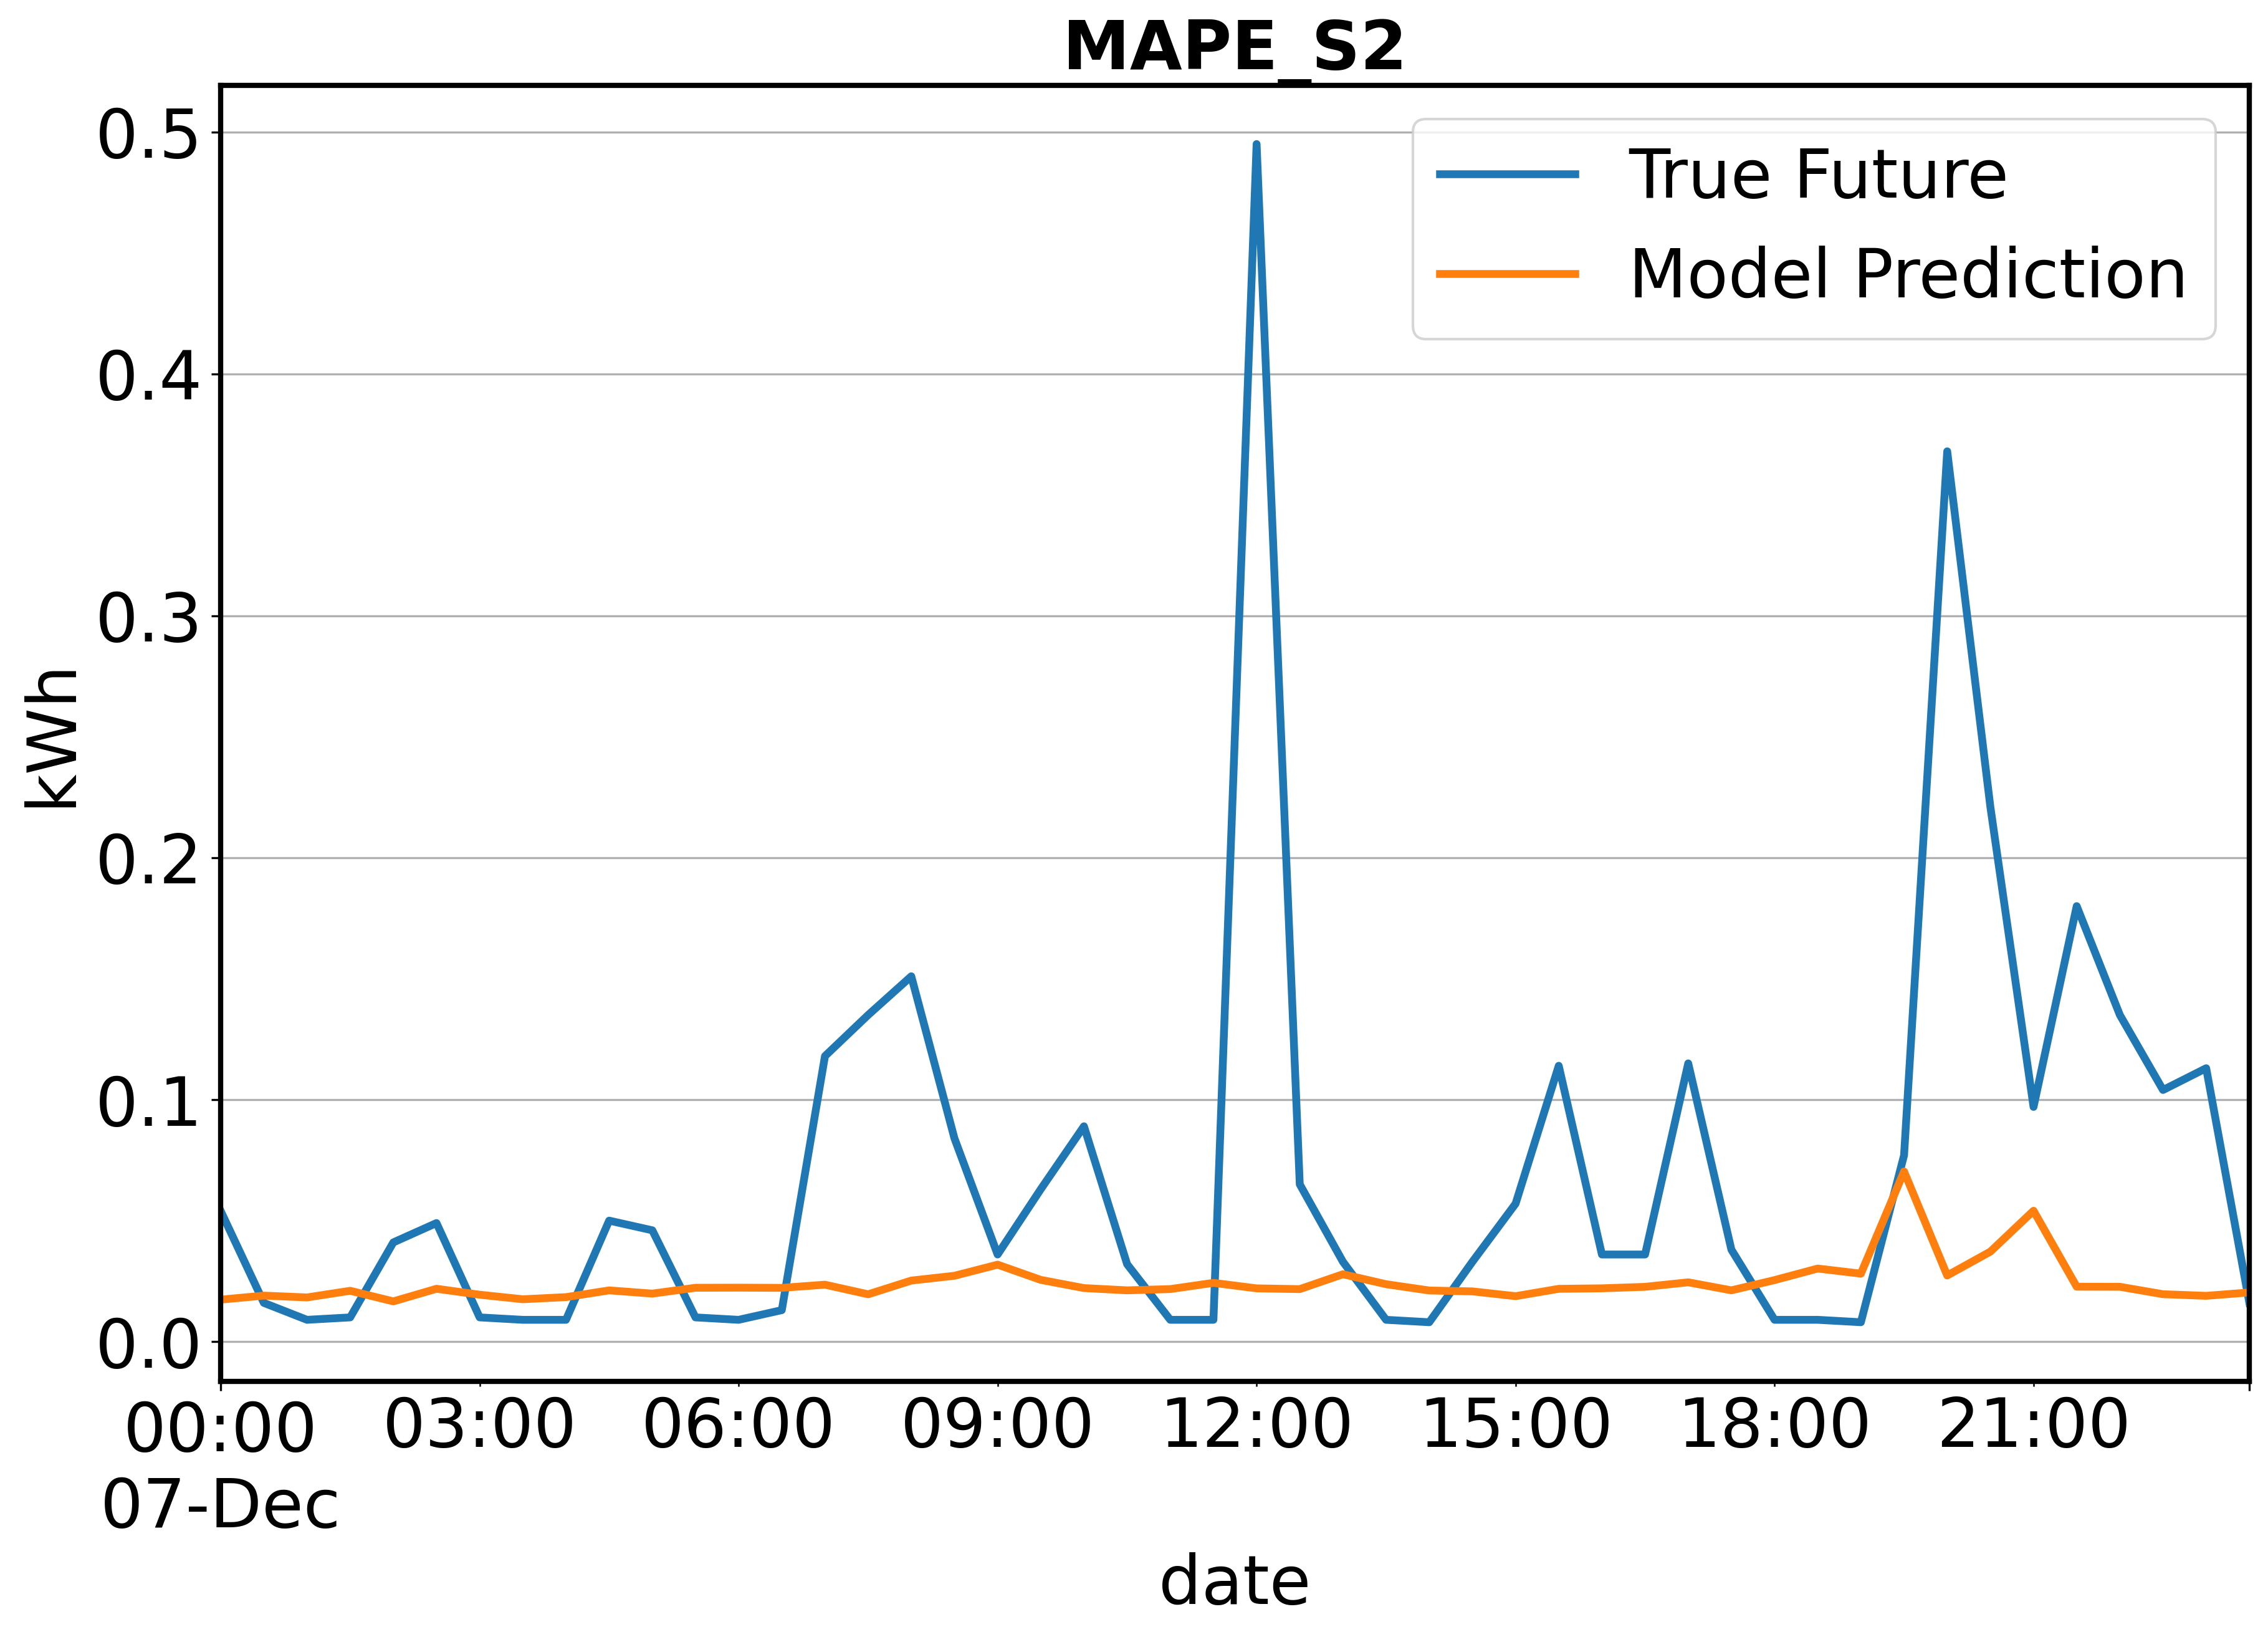
\includegraphics[width=1\linewidth]{IDMAPE_S2_Day341.png}
		\caption{MAPE forecast - Serie $ 2 $}
	\end{subfigure}	
	\begin{subfigure}{0.32\textwidth}
		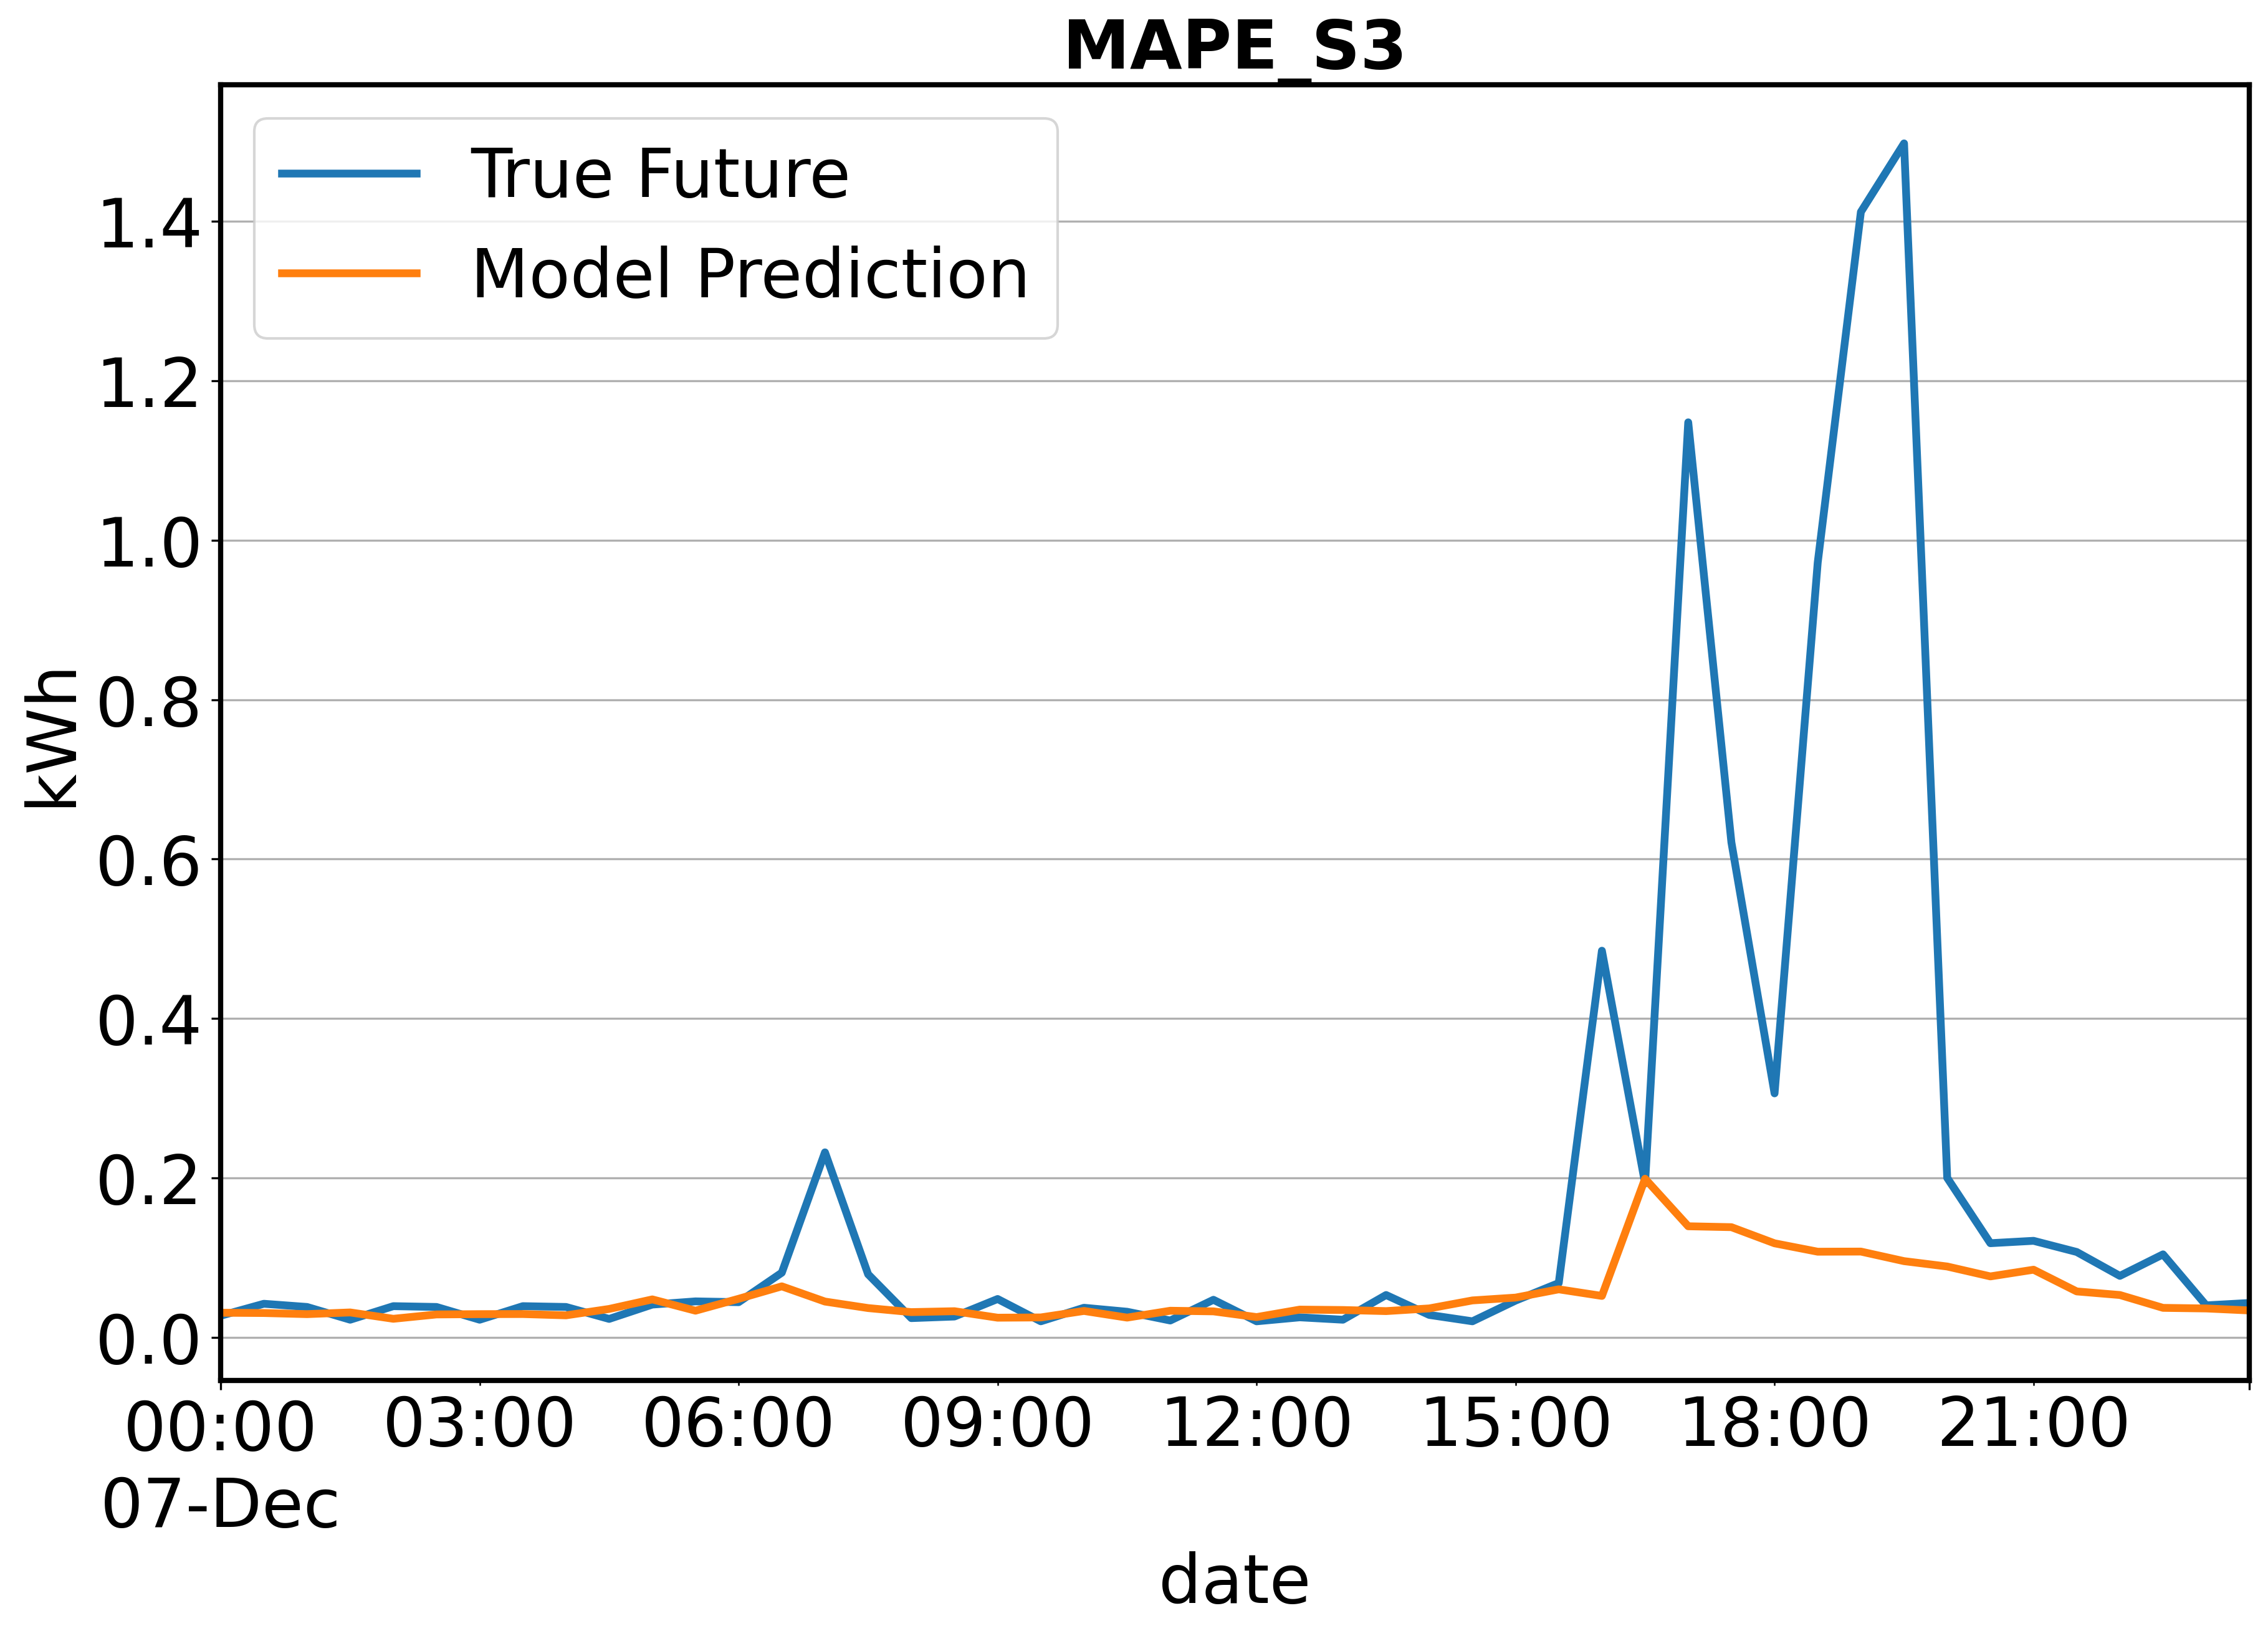
\includegraphics[width=1\linewidth]{IDMAPE_S3_Day341.png}
		\caption{MAPE forecast - Serie $ 3 $}
	\end{subfigure}
 	\caption{The prediction results of the different models on 7th December. (True values: blue/ Prediction: orange)}
 	\label{fig:individual_forecasts}
 \end{figure}


First, it is again stressed that the ``mean squared error'' is chosen as metric during training of the LSTM models. Because of this, the LSTM models are more pushed towards learning the peaks of the reference signal due to the squared error. It can be seen that on the $ 7^{th} $ of December, the peaks of Serie 1 and Serie 3 are present in the predicted signal. It was found that especially for Serie 1, the LSTM models are predicting a higher consumption than the reference signal. The shape of the reference and prediction signals are similar, but there is an offset between the two signals. A reason for the shift could be that the LSTM models are trained using the MSE metric. It is found in literature that when a least square fitting is performed on data points the curve that is fitted can be much disturbed by the presence of outliers. The disturbance resulted also in a shift of the fitted curve. Because during training the MSE is used, the peaks during the day also act as outliers that could be responsible for the model shift. A solution to solve this is to get rid of the squared error and punish more proportional by using the MAE metric instead. On the other hand it can be argued that it is better to predict a higher consumption that one that is too low, because it is better to anticipate to a worse scenario then expected.\\

The reader is reminded that there is no regulation added for Model 1: Serie 1 and Model 3: Serie 1 and 3. When regularization is added this is clearly visible in Figure \ref{fig:individual_forecasts} because without regulation the predicted signal is much more choppy. A clear example can be seen for Model 2 and 3 in serie 3. These two models both show a small bump in the predicted signal before the larger peak. Model 2 where a form of regularization is added shows a very smooth bump while in Model 3 without regularization, the bump is much more choppy. \\

It can be seen that the ``mean forecast'' is able to identify the two peaks in Serie 1 and the large peak in Serie 3, but as is expected from a mean, this peak is smaller due to averaging. The ``mean forecast'' method however suffers less from the offset than the LSTM models in Serie 1.\\

As expected the ``MAPE forecast'' will focus on correctly predicting the low values in the reference signal because these will get in the denominator of the MAPE metric according to Eq. \ref{eq:MAPE}. It can be seen that the peaks will be ignored when this method is applied. 

\section{Conclusion}
In this chapter the performance of the developed models is assessed. Firstly, the model selection was discussed and it was explained that the models obtained after the parameter search are ran ten times with different initialized weight matrices. The one that performed best on the validation was selected. The number of epochs that the models trained was low, except for model 2 and 3 on Serie 2.\\

 Secondly, the performance on the test set is discussed for the LSTM models and two baseline models using bar plots that displayed the MAE on the test set for each serie. It was concluded that there is a reduction for all the three LSTM models in comparison to both the baseline models for Serie 2 and 3. Also, Model 2 always performed worse based on MAE then the other LSTM models and it can be concluded that the flattening layer didn't have much effect.\\ 
 $ 7 $ December is chosen for which all the predicted signals are grouped for the different models. From this figure is was clear that the LSTM models are able to identify peaks of the reference signal and they have the same overall shape. Predicting the peaks correctly is an important, practical feature e.g. to anticipate electrical peak consumption demands. It was also noticed that the predictions are often an overestimation of the reference signal. Especially for Serie 1, the shape of the reference and prediction signals are similar, but there is an offset between the two signals. The offset could possibly be reduced with another choice of error metric during training. However, it can be a serie dependent effect due to the fact that only for Serie 1 there is a large offset at the start. It can be argued that in practice it is better to overestimate, than underestimate. Because of the overestimation on small values, it was found that the MAPE of the three LSTM neural networks performed worse than the baseline models. Also, the influence of adding regularization could be seen which leads to more smooth signals.\\
 
The ``mean forecast'' baseline model was not able to predict the peaks in the reference signal as good as the LSTM models, but it has a lower offset error in Serie 1. The ``MAPE forecast'' is focussed on predicting all the small values correct to minimize the MAPE, but ignores all the peaks of the reference signal.
 


%%% Local Variables: 
%%% mode: latex
%%% TeX-master: "thesis"
%%% End: 

\chapter{Conclusion}
\label{cha:conclusion}
The final chapter contains the overall conclusion. It also contains
suggestions for future work and industrial applications.

\section{Future work}

- because it was seen that much forecasts have the correct form with regard to the amount of peaks a first thing to try to solve this could be to adjust the error metric that is used during training from MSE to MAE. The peaks will be more proportional punished and this could lead that the model shifts down. 
- genetic algorithm to tune the parameters

%%% Local Variables: 
%%% mode: latex
%%% TeX-master: "thesis"
%%% End: 


% Indien er bijlagen zijn:
\appendixpage*          % indien gewenst
\appendix
\chapter{Introduction to the dataset}
\label{app:A}
Appendices hold useful data which is not essential to understand the work
done in the master's thesis. An example is a (program) source.
An appendix can also have sections as well as figures and references\cite{h2g2}.

\section{Introduction to the dataset}

\begin{figure}[h!]
	\centering
	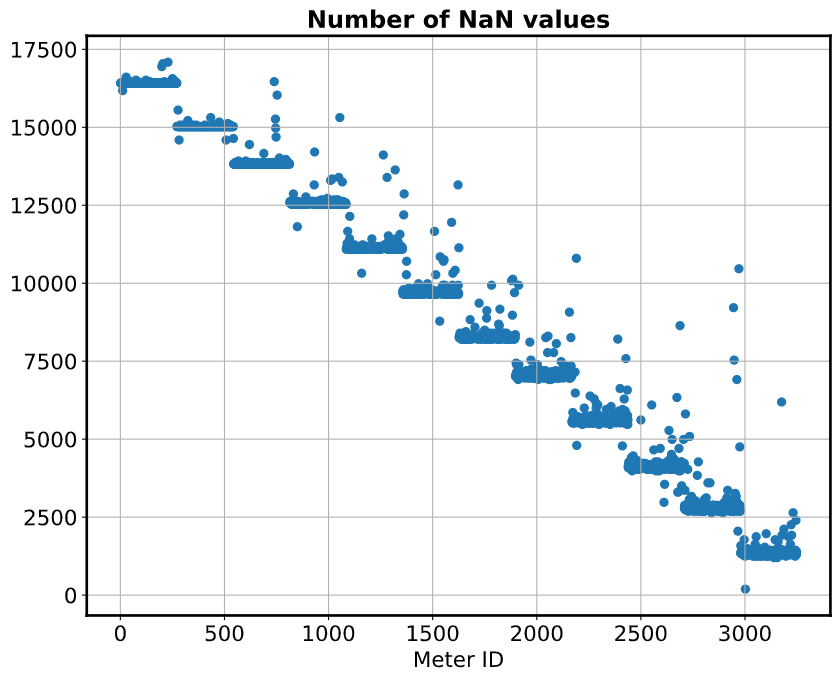
\includegraphics[width=0.8\textwidth]{amountNaN.png}
	\caption{The amount of NaN values in all the 3248 smart meters.}
	\label{fig:amountNaN}
\end{figure}

\begin{table}[h]
	\centering
	\begin{tabular}{|p{5cm}|p{2.5cm}|}
		\hline
		\textbf{Attribute} & \textbf{Filled places}\\ \hline	
		Dwelling type  & 1702\\ \hline
		\# Occupants & 74\\ \hline
		Heating fuel & 1859\\ \hline
		Heating fuel & 78\\ \hline
		Hot water fuel & 76\\ \hline
		Boiler age & 74\\ \hline
		Loft insulation & 75\\ \hline
		Wall insulation & 75\\ \hline
		Heating temperature & 74\\ \hline
		Efficient lighting percentage & 73\\ \hline
		Dishwasher & 76\\ \hline
		Freezer & 70\\ \hline
		Fridge freezer & 70\\ \hline
		Refrigerator & 73\\ \hline
		Tumble Dryer & 76\\ \hline
		Washing machine & 76\\ \hline
		Game console &72\\ \hline
		Laptop & 70\\ \hline
		Pc & 70\\ \hline
		Router & 69\\ \hline
		Set top box & 70\\ \hline
		Tablet & 70\\ \hline
		Tv & 75\\ \hline
		
	\end{tabular}
	\caption{Amount of response on the voluntary questionnaires. }
	\label{tab:attributes}
\end{table}

\section{Missing values}

\begin{figure}[h!]
	\centering
	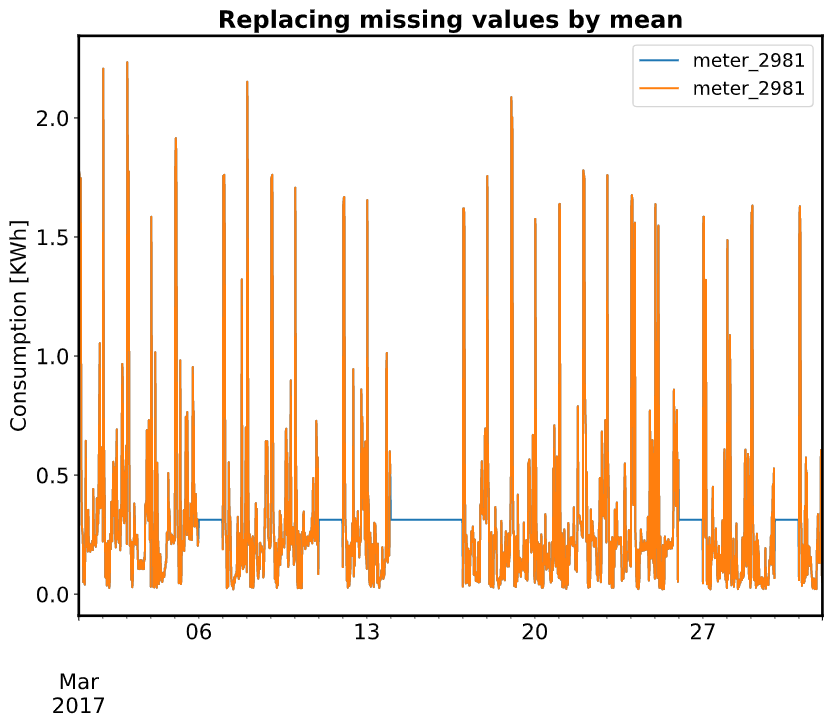
\includegraphics[width=0.8\textwidth]{mv_mean.png}
	\caption{Resulting month of March after substitution of the missing values by the mean value of the measurements. }
	\label{fig:mv_mean}
\end{figure}

\begin{figure}[h!]
	\centering
	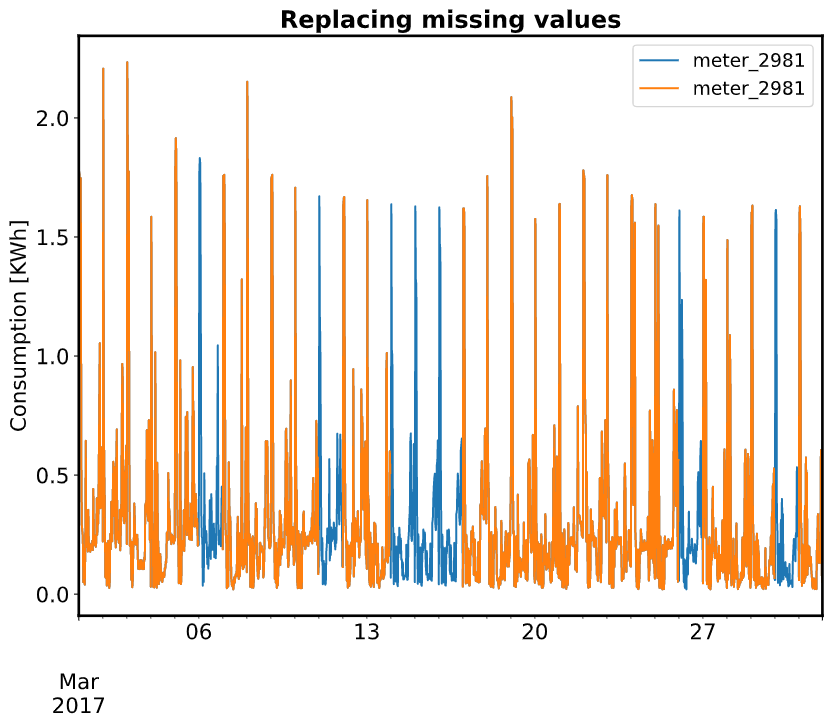
\includegraphics[width=0.8\textwidth]{mv_s.png}
	\caption{Resulting month of March after substitution of the missing values by the mean value of the same moment on the next and previous day.}
	\label{fig:mv_s}
\end{figure}

\section{Untraditional behaviour of the measurements}

\subsection{Zeros days}
\begin{figure}[h!]
	\centering
	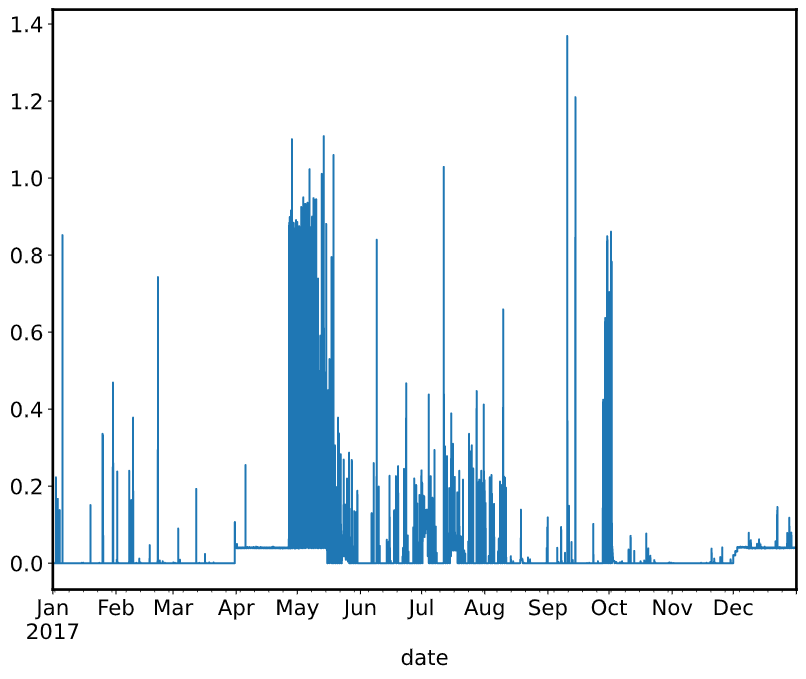
\includegraphics[width=0.8\textwidth]{zero_con.png}
	\caption{One of the $9$ identified meters with multiple zero daily consumptions}
	\label{fig:zero_con}
\end{figure}


\subsection{Fundamental change}

\begin{figure}[h!]
	\centering
	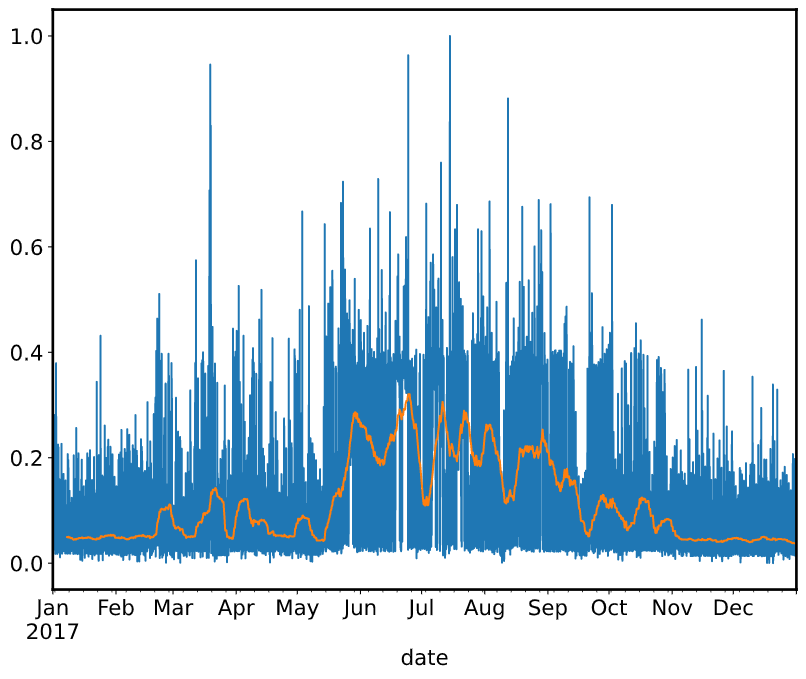
\includegraphics[width=0.8\textwidth]{fundamental_change.png}
	\caption{The time-serie with the original maximum difference between the minimum and maximum weekly rolling averages.}
	\label{fig:fundamental_change}
\end{figure}

\begin{figure}[h!]
	\centering
	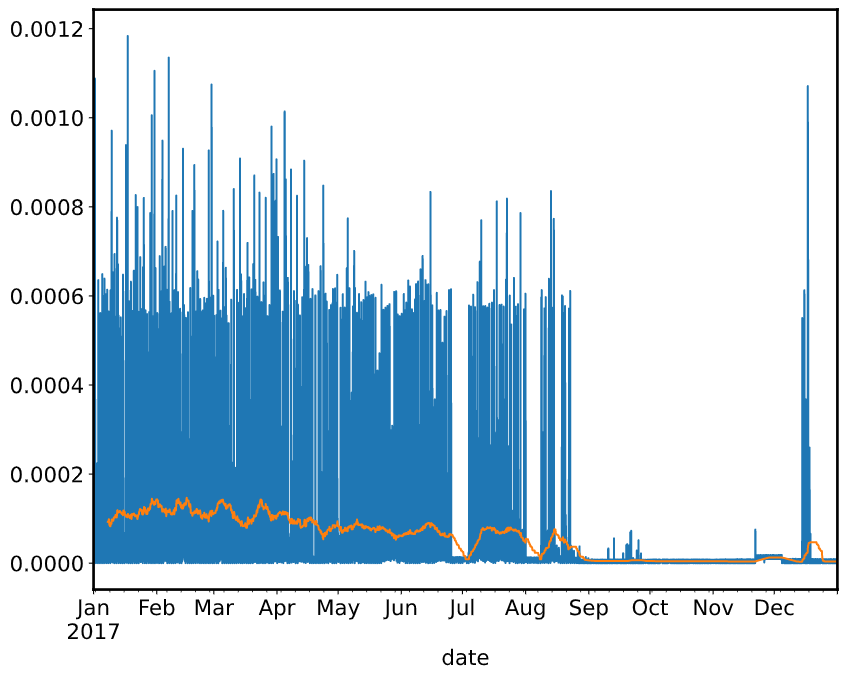
\includegraphics[width=0.8\textwidth]{f_c.png}
	\caption{The time-serie with the new maximum difference between the minimum and maximum weekly rolling averages.}
	\label{fig:f_c}
\end{figure}



%%% Local Variables: 
%%% mode: latex
%%% TeX-master: "thesis"
%%% End: 

\chapter{Forecasting the daily electricity consumption - extra}
\label{app:B}

In this appendix extra information and Figures are added that are not necessary to understand the work discussed in Chapter \ref{cha:Forecasting the daily electricity consumption}.

\section{Baseline models}

 \begin{figure}[h]
	\centering
	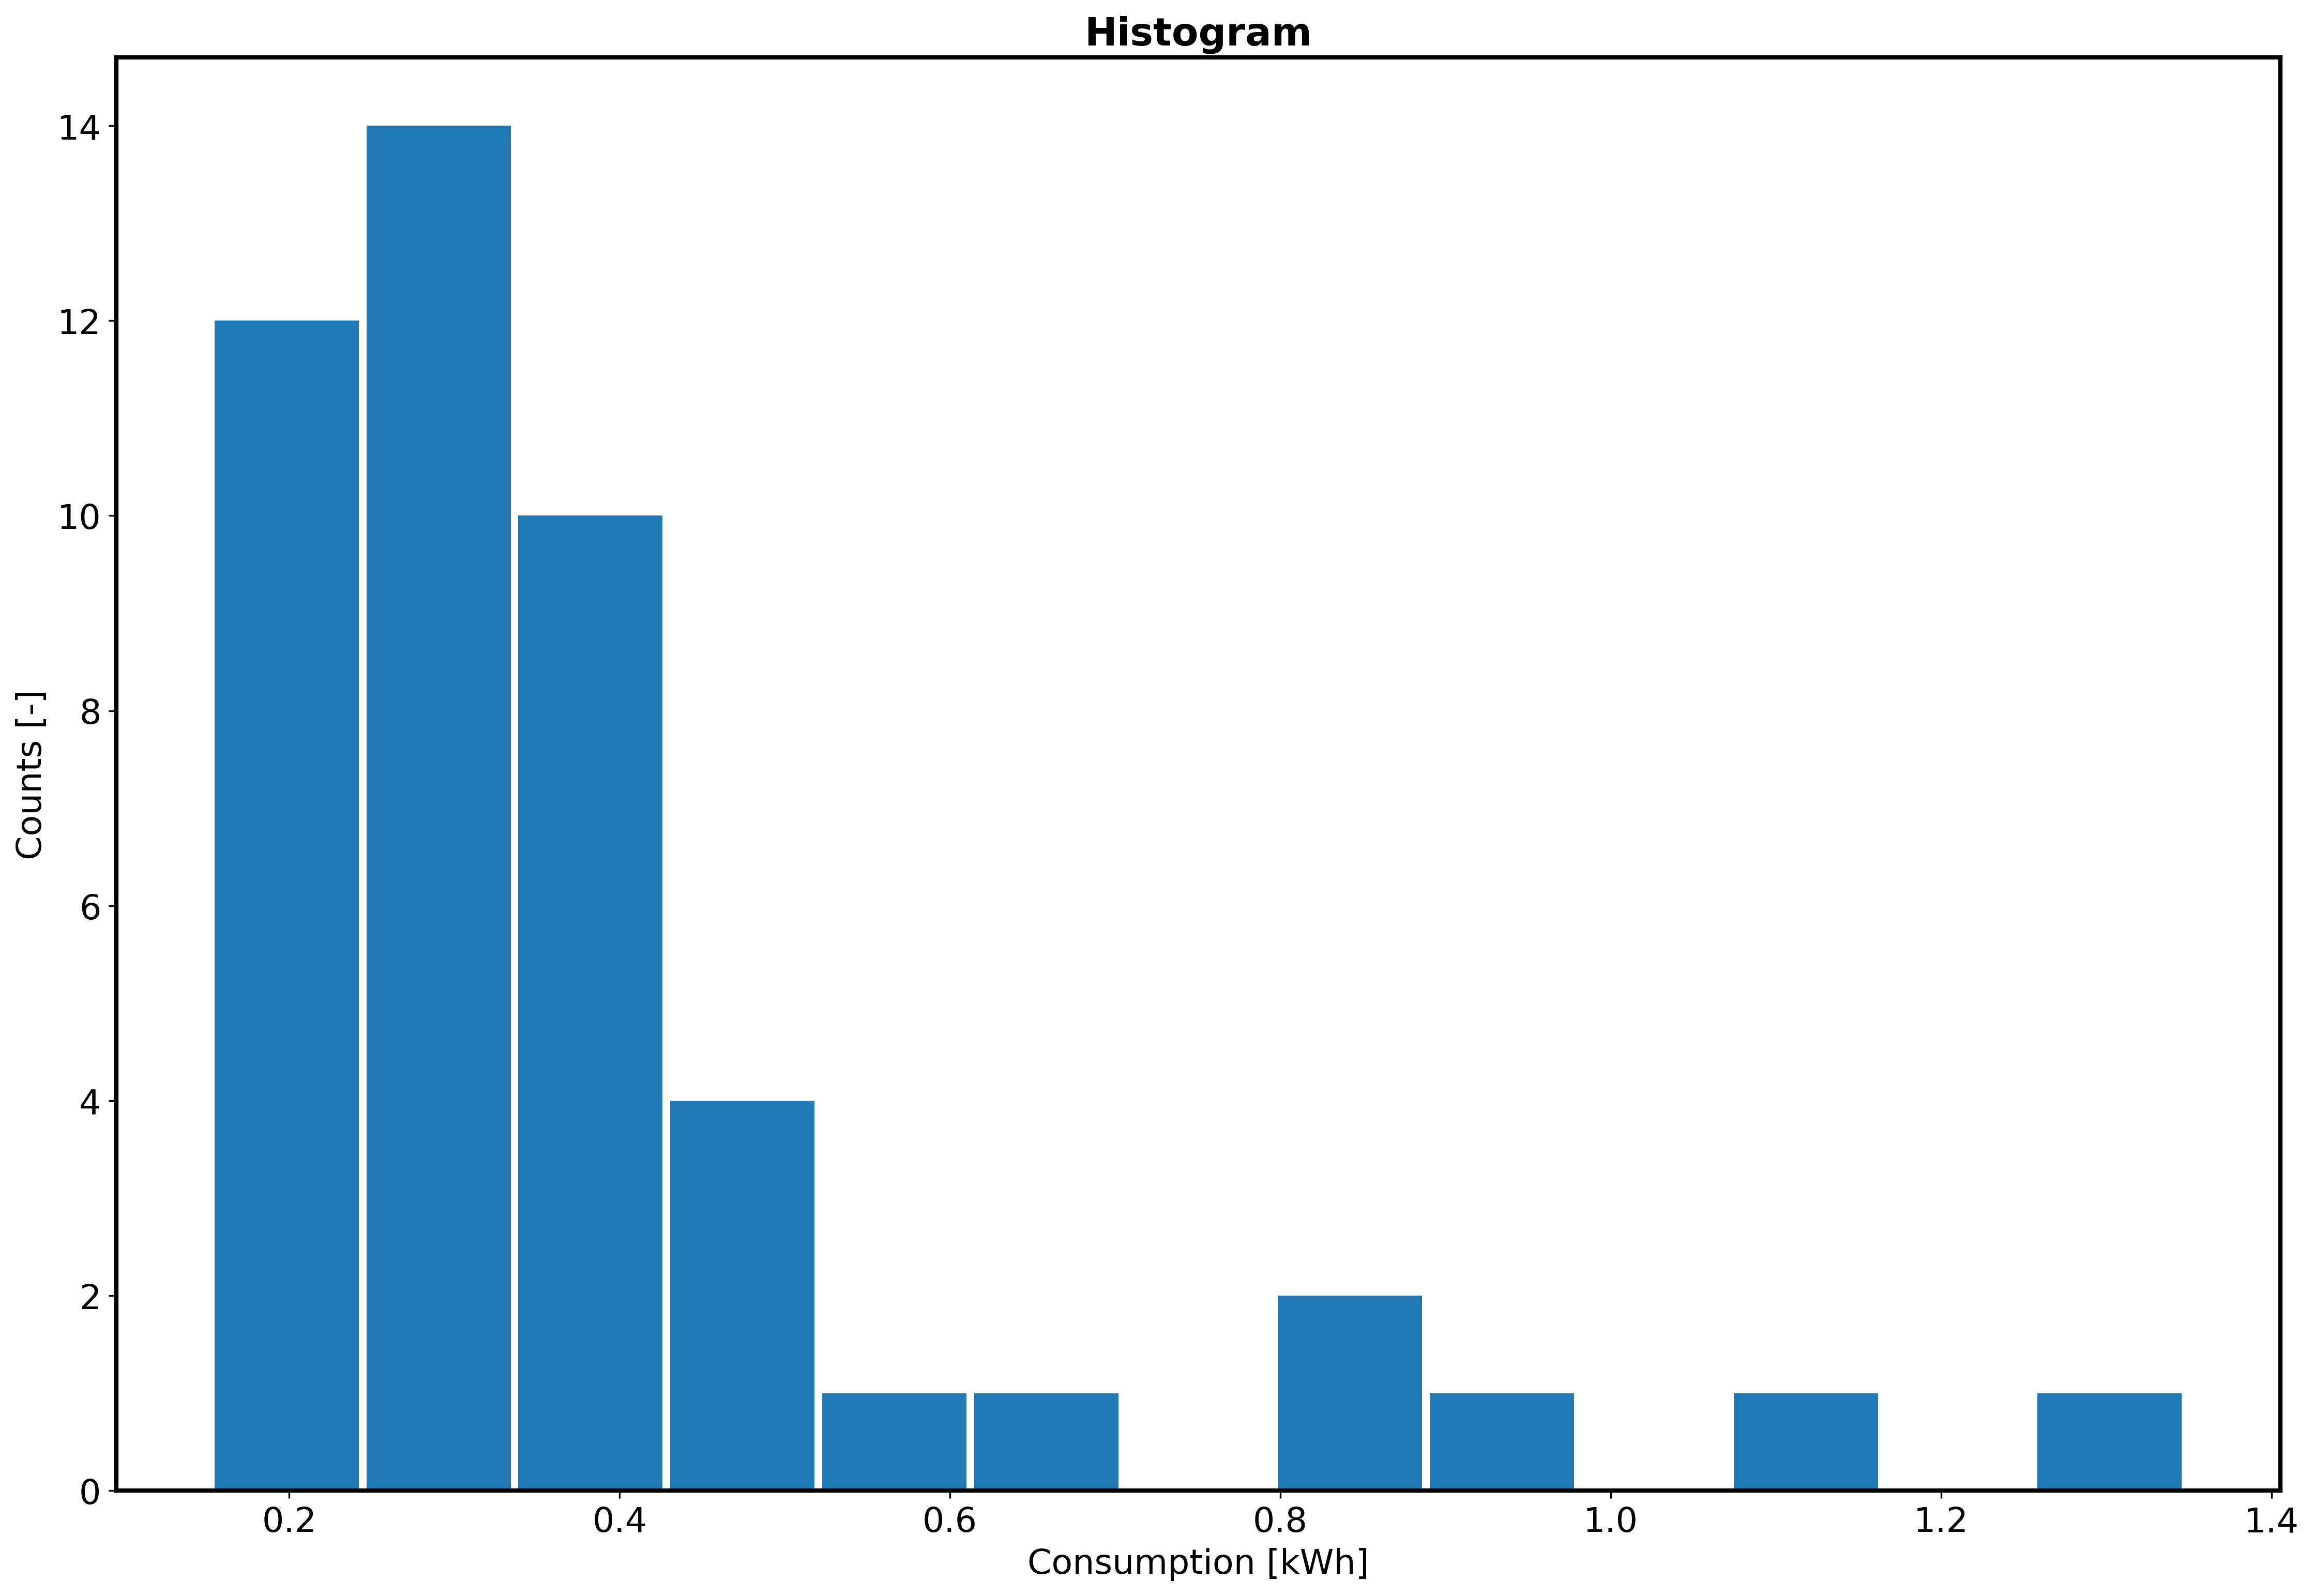
\includegraphics[width=0.8\linewidth]{histogram_mape.png}
	\caption{An example histogram of the consumption in [kWh] versus count [-] used during MAPE forecast.}
	\label{fig:histogram_mape}
\end{figure}

\section{Parameter Search}

\subsection{Model 2}

\begin{table}[h]
	\centering
	\begin{tabular}{@{}l||c|ccc@{}} \toprule
		\multicolumn{5}{c}{Model 2: Stateless (flatten layer)}\\\midrule\midrule
		\textbf{Chosen parameter}	& \textbf{Value} & \textbf{Serie $ 1 $} & \textbf{Serie $ 2 $} & \textbf{Serie $ 3 $}\\\midrule
		Hidden states LSTM & $ 20 $ & $0.446 $&$ 0.0622 $  & \\
		& $ 50 $  & 		  		&		   				& $0.319 $		\\\hline
		layers LSTM & $ 1 $ & 		&		   & 		\\
		& $ 3 $ &  $21.3 $   	&$ 10.60 $  				& $9.98$\\\hline
		Lag value & $ 48 $ & $7.51 $&$ 2.84 $		   & \\
		& $ 96 $ &          		& 		 & 	$1.76$	\\\hline
		Learning rate & $ 10^{-2} $ &       &		 & 		\\
		& $  10^{-3} $ &$23.4 $    &$ 2.51$  			& $13.2$\\
		& $  10^{-4} $ &$43.0 $		&$ 12.8$    	& $17.9$\\\bottomrule
		
	\end{tabular}
	\caption{Each value in this table shows the average error when the corresponding parameter value is used, normalized by the biggest error of the possible values of one parameter and finally subtracted by one. Therefore, each value shows a percentage of improvement with respect to the worst value for one parameter for each serie during phase $ 1 $ of the parameter search.}
	\label{tab:relative_performance_parameters_phase_one_model_two}
\end{table}

\begin{table}[h]
	\centering
	\begin{tabular}{@{}l|ccc@{}} \toprule
		\multicolumn{4}{c}{Model 2: Stateless (flatten layer)}\\\midrule\midrule
		\textbf{Parameters}	& \textbf{Serie $ 1 $} & \textbf{Serie $ 2 $} & \textbf{Serie $ 3 $}\\\midrule
		Hidden states LSTM & $20 $&$ 50 $  & $50 $\\
		layers LSTM & $3 $&$ 3 $  & $3$\\
		Lag value & $96 $&$ 48$  & $96$\\
		Learning rate & $0.001 $&$ 0.0001$  & $0.001$\\\hline
		MAE error 1   & $ 0.137 $ & $ 0.0426 $ & $ 0.0973 $\\
		MAE error 2   & $ 0.139 $ & $ 0.0430 $ & $ 0.107 $\\
		MAE error 3   & $ 0.136 $ & $ 0.0424 $ & $ 0.100 $\\\bottomrule
	\end{tabular}
	\caption{The values of the parameters with the lowest average MAE on the validation set over three runs.}
	\label{tab:best_performing_para_phase1_model2}
\end{table}


\begin{figure}[h]
	\centering
	\begin{subfigure}{0.49\linewidth}
		\includegraphics[width=1\linewidth]{serie1_model2.png}
		\caption{Model 2}
	\end{subfigure}	
	\begin{subfigure}{0.49\linewidth}
		\includegraphics[width=1\linewidth]{serie2_model2.png}
		\caption{Model 2}
	\end{subfigure}
	\begin{subfigure}{0.5\linewidth}
		\includegraphics[width=1\linewidth]{serie3_model2.png}
		\caption{Model 2}
	\end{subfigure}
	\caption{Results of the sensitivity analysis on the size of the regularization parameter and the dropout rate according to MAE.(Legend: \textit{r\_D}: regularization size of weights of DENSE layer,  \textit{r\_r\_L}: regularization size of recurrent weight of LSTM, \textit{r\_L}: regularization size of input weights of LSTM, \textit{d\_L}: dropout rate of inputs LSTM, \textit{r\_d\_L}: dropout rate of hidden states LSTM, \textit{d\_D}: dropout rate of DENSE layer, \textit{or}: best performing serie from phase one)}
	\label{fig:sensitivity_model2}
\end{figure}

\begin{figure}[h]
	\centering
	\begin{subfigure}{0.49\linewidth}
		\includegraphics[width=1\linewidth]{learning_rate_serie1_model2.png}
		\caption{Model 2}
	\end{subfigure}	
	\begin{subfigure}{0.49\linewidth}
		\includegraphics[width=1\linewidth]{learning_rate_serie2_model2.png}
		\caption{Model 2}
	\end{subfigure}
	\begin{subfigure}{0.5\linewidth}
		\includegraphics[width=1\linewidth]{learning_rate_serie3_model2.png}
		\caption{Model 2}
	\end{subfigure}
	\caption{The evaluation of the error on the validation set in function of the learning rate size.}
	\label{fig:learning_rate_model2}
\end{figure}

\clearpage
\subsection{Model 3}

\begin{table}[ht]
	\centering
	\begin{tabular}{@{}l||c|ccc@{}} \toprule
		\multicolumn{5}{c}{Model 3: Stateful (1 time step)}\\\midrule\midrule
		\textbf{Chosen parameter}	& \textbf{Value} & \textbf{Serie $ 1 $} & \textbf{Serie $ 2 $} & \textbf{Serie $ 3 $}\\\midrule
		Hidden states LSTM & $ 20 $ & $6.66 $		&  & $0.55 $\\
		& $ 50 $ & 		  		&	$ 0.51 $	   & 		\\\hline
		layers LSTM & $ 1 $ & $30.00 $		&	$ 1.52 $	   & 	$7.42$	\\
		& $ 3 $ & 	      		& 			 & \\\hline
		Learning rate & $ 10^{-2} $ &       &		   & 		\\
		& $  10^{-3} $ &$17.72 $&$0.0$  & $0.0$\\
		& $  10^{-4} $ &$27.28 $&$ 2.28$    & $11.13$\\\bottomrule
		
	\end{tabular}
	\caption{Each value in this table shows the average error when the corresponding parameter value is used, normalized by the biggest error of the possible values of one parameter and finally subtracted by one. Therefore, each value shows a percentage of improvement with respect to the worst value for one parameter for each serie during phase $ 1 $ of the parameter search.}
	\label{tab:relative_performance_parameters_phase_one_model_three}
\end{table}

\begin{table}[ht]
	\centering
	\begin{tabular}{@{}l|ccc@{}} \toprule
		\multicolumn{4}{c}{Model 3: Stateful (1 time step)}\\\midrule\midrule
		\textbf{Parameters}	& \textbf{Serie $ 1 $} & \textbf{Serie $ 2 $} & \textbf{Serie $ 3 $}\\\midrule
		Hidden states LSTM  & $50 $&$ 50 $  & $20 $\\
		layers LSTM & $1 $&$ 1 $  & $1$\\
		Learning rate & $0.0001 $&$ 0.0001$  & $0.0001$\\\hline
		MAE error 1   & $ 0.132 $ & $ 0.0522 $ & $ 0.109 $\\
		MAE error 2   & $ 0.130 $ & $ 0.0613 $ & $ 0.111 $\\
		MAE error 3   & $ 0.138 $ & $ 0.0570 $ & $ 0.112 $\\\bottomrule
	\end{tabular}
	\caption{The values of the parameters with the lowest average MAE on the validation set over three runs.}
	\label{tab:best_performing_para_phase1_model3}
\end{table}

\begin{figure}[ht]
	\centering
	\begin{subfigure}{0.49\linewidth}
		\includegraphics[width=1\linewidth]{serie1_model3.png}
		\caption{Model 3}
	\end{subfigure}	
	\begin{subfigure}{0.49\linewidth}
		\includegraphics[width=1\linewidth]{serie2_model3.png}
		\caption{Model 3}
	\end{subfigure}
	\begin{subfigure}{0.5\linewidth}
		\includegraphics[width=1\linewidth]{serie3_model3.png}
		\caption{Model 3}
	\end{subfigure}
	\caption{Results of the sensitivity analysis on the size of regulation parameter and the dropout rate with respect to the mean absolute error.(Legend: \textit{r\_r\_L}: regularization size of recurrent weight of LSTM, \textit{r\_L}: regularization size of input weights of LSTM and \textit{or}: best performing serie from phase one)}
	\label{fig:sensitivity_model3}
\end{figure}

\begin{figure}[h]
	\centering
	\begin{subfigure}{0.49\linewidth}
		\includegraphics[width=1\linewidth]{learning_rate_serie1_model3.png}
		\caption{Model 3}
	\end{subfigure}	
	\begin{subfigure}{0.49\linewidth}
		\includegraphics[width=1\linewidth]{learning_rate_serie2_model3.png}
		\caption{Model 3}
	\end{subfigure}
	\begin{subfigure}{0.5\linewidth}
		\includegraphics[width=1\linewidth]{learning_rate_serie3_model3.png}
		\caption{Model 3}
	\end{subfigure}
	\caption{The evaluation of the error on the validation set in function of the learning rate size.}
	\label{fig:learning_rate_model3}
\end{figure}





%%% Local Variables: 
%%% mode: latex
%%% TeX-master: "thesis"
%%% End: 

\chapter{Extensions on the evaluation results}
\label{app:Extensions on the evaluation results}

\section{Results on the testset}

\begin{figure}[h]
	\centering
	\includegraphics[width=0.8\linewidth]{MAE_1_line.png}
	\caption{The MAE performance for the different days in the test set for Serie 1.}
	\label{fig:MAE_line_serie1}
\end{figure}

\begin{figure}[h]
	\centering
	\includegraphics[width=0.8\linewidth]{MAE_2_line.png}
	\caption{The MAE performance for the different days in the test set for Serie 2.}
	\label{fig:MAE_line_serie2}
\end{figure}	

\begin{figure}[h]
	\centering
	\includegraphics[width=0.8\linewidth]{MAE_3_line.png}
	\caption{The MAE performance for the different days in the test set for Serie 3.}
	\label{fig:MAE_line_serie3}
\end{figure}









%\section{Old stuff}
%\subsection{Removing outliers}


% some meters don't have a lot of missing values, but have very untraditional output. Two cases are looked into
% 1. big deviation from the average meter. 
% 2. a full day of zeros is included. 
% 3. the moving average changes spectaculair --> fundamental change in the energy consumption
% whitch is hard to forecast for. (not consistent with a normal consumption pattern)
% Weird meters that are identified: 2985, 2984,
% Normal meters: 2979, 2982
% idea to check also for outliers on monthly/weekly scale? 
%After the missing values are replaced by estimations, the outliers of the electricity consumption signals are identified.
%This is done by looking  at the z-scores of the yearly consumptions. A z-score is calculated using equation \ref{eq:z-score} and assumes that the yearly consumptions are normally distributed around the average consumption. Consumptions that have a very low probability to occur are removed by imposing that $ |z-score| < 3 $.

%\begin{equation}
%	z-score = \frac{x-\mu}{\sigma}
%\end{equation}                      
%
%Figure \ref{fig:z-score} gives the obtained z-values. It can be seen that $ 6 $ meters with an unlikely high or low consumption are removed. 
%
%\begin{figure}[h!]
%	\centering
%	\includegraphics[width=0.8\textwidth]{z-score.png}
%	\caption{Z-scores calculated from the yearly consumptions.}
%	\label{fig:z-score}
%\end{figure}


%\subsection{Normalization of the data}
%% normalize as done in ppt --> deviding by the yearly consumption.
%% downside of this normalilzation that outshooters will have influence.
%Normalization is necessary because while absolute consumption differs, relative patterns of human behaviour are more similar \cite{Lago2020}. The patterns in the human behaviour is what a forecasting model is trying to predict and normalization contributes by avoiding the disturbance of different magnitudes in which this human pattern may occur. Every individual household time-serie is normalized based on its maximum and minimum value according to equation \ref{eq:norm}. 
%
%\begin{equation}\label{eq:norm}
%	normalized value = \frac{x - x_{min}}{x_{max} - x_{min}}
%\end{equation}  
%
%As discussed in section \ref{s:Basic analysis} the average is taken over all the normalized time-series to obtain a single signal.\textbf{Ask if this is good??}  Because the maximum is taken into account during the normalization, measurement out shooters have an influence on the normalization. 


%\section{ARIMA}
%% Idea is to use the simple ARIMA model as a base line forecasting model. 
%% see datacamp and youtube Lola
%% ARIMA assumes stationary data.
%What is ARIMA. 
%Assumptions of ARIMA...
%
%\textbf{Stationarity}\\
%https://machinelearningmastery.com/remove-trends-seasonality-difference-transform-python/
%When data is modelled it is assumed that the statistics of the data are consistent or stationary. This means the mean and standard deviation is not changing in time. However, because time series are often subdued to a trend or seasonality this assumption of stationarity is violated. In order to model not stationary observations by a stationary model as ARIMA, trends and seasonal effects should be removed. A way to check the stationarity of your observations, the ``Dicky-Fuller test'' can be used.
%A way to remove non-stationarity is by using ``Difference Transform''. Here the trend and seasonality is subtracted from the observations leaving behind a stationary dataset.


%%% Local Variables: 
%%% mode: latex
%%% TeX-master: "thesis"
%%% End: 


\backmatter
% Na de bijlagen plaatst men nog de bibliografie.
% Je kan de  standaard "abbrv" bibliografiestijl vervangen door een andere.
\bibliographystyle{abbrv}
\bibliography{Time_Series}

\end{document}

%%% Local Variables: 
%%% mode: latex
%%% TeX-master: t
%%% End: 
